% main.tex
% 概率论笔记
% 编译：XeLaTeX
\documentclass[10pt]{book}

% ── 加载所有配置 ──
% preamble/packages.tex
% 概率论笔记 —— 宏包加载
\usepackage{ctex}
\usepackage{amsmath, amsthm, amssymb, amsfonts, mathrsfs}
\usepackage{graphicx}
\usepackage{setspace}
\usepackage{geometry}
\usepackage{float}
\usepackage{hyperref}
\usepackage[backend=biber,style=ieee]{biblatex}
\usepackage{framed}
\usepackage[dvipsnames]{xcolor}
\usepackage[most]{tcolorbox}
\tcbuselibrary{theorems}
\tcbuselibrary{breakable}
\usepackage{fontspec}
\usepackage{xeCJK}
\usepackage{tikz}
\usetikzlibrary{arrows.meta, positioning}
\usepackage{fancyhdr}

% preamble/colors.tex
% ------------------------------------
% 配色方案：绿色系主题 + 金饰
% 用于概率论笔记
% ------------------------------------

% ---- 绿色系 —— 主结构色 ----
\definecolor{GreenMain}{RGB}{0, 128, 64}
\definecolor{GreenLight}{RGB}{102, 204, 128}
\definecolor{GreenDark}{RGB}{0, 102, 51}
\definecolor{GreenAccent}{RGB}{51, 204, 102}

% ---- 暖金色系（Gold）—— 章节扉页装饰 ----
\definecolor{GoldDark}{RGB}{140, 100, 35}
\definecolor{GoldMain}{RGB}{178, 132, 55}
\definecolor{GoldLight}{RGB}{210, 172, 100}
\definecolor{GoldPale}{RGB}{242, 230, 205}

% ---- 兼容旧名称 ----
\colorlet{ProbGreen}{GreenMain}
\colorlet{ProbLightGreen}{GreenLight}
\colorlet{ProbDarkGreen}{GreenDark}
\colorlet{ProbAccentGreen}{GreenAccent}
\colorlet{BlueMain}{GreenMain}
\colorlet{BlueDark}{GreenDark}
\colorlet{BlueLight}{GreenLight}
\colorlet{BlueAccent}{GreenAccent}

% preamble/theorems.tex
% ------------------------------------
% 概率论定理环境（绿色系 tcolorbox）
% ------------------------------------

% ---- 定义 ----
\newtcbtheorem[number within=section]{mydefinition}{定义}{
	breakable, enhanced,
	colback=white, colframe=GreenMain,
	arc=4pt, boxrule=0.8pt, leftrule=4pt,
	fonttitle=\bfseries\theoremFont,
	fontupper=\normalsize\CJKfamily{theoremCJK},
	left=16pt, right=12pt, top=10pt, bottom=10pt,
	before skip=12pt, after skip=12pt,
	boxsep=4pt, left skip=16pt,
}{def}

% ---- 定理 ----
\newtcbtheorem[use counter from=mydefinition]{mytheorem}{定理}{
	breakable, enhanced,
	colback=white, colframe=GreenMain,
	arc=4pt, boxrule=0.8pt, leftrule=4pt,
	fonttitle=\bfseries\theoremFont,
	fontupper=\normalsize\CJKfamily{theoremCJK},
	left=16pt, right=12pt, top=10pt, bottom=10pt,
	before skip=12pt, after skip=12pt,
	boxsep=4pt, left skip=16pt,
}{th}

% ---- 命题 ----
\newtcbtheorem[use counter from=mydefinition]{proposition}{命题}{
	breakable, enhanced,
	colback=white, colframe=GreenMain,
	arc=4pt, boxrule=0.8pt, leftrule=4pt,
	fonttitle=\bfseries\theoremFont,
	fontupper=\normalsize\CJKfamily{theoremCJK},
	left=16pt, right=12pt, top=10pt, bottom=10pt,
	before skip=12pt, after skip=12pt,
	boxsep=4pt, left skip=16pt,
}{prop}

% ---- 推论 ----
\newtcbtheorem[use counter from=mydefinition]{mycorollary}{推论}{
	breakable, enhanced,
	colback=white, colframe=GreenLight,
	arc=4pt, boxrule=0.8pt, leftrule=4pt,
	fonttitle=\bfseries\theoremFont,
	fontupper=\normalsize\CJKfamily{theoremCJK},
	left=16pt, right=12pt, top=10pt, bottom=10pt,
	before skip=12pt, after skip=12pt,
	boxsep=4pt, left skip=16pt,
}{cor}

% ---- 公理 ----
\newtcbtheorem[use counter from=mydefinition]{myaxiom}{公理}{
	breakable, enhanced,
	colback=white, colframe=GreenDark,
	arc=4pt, boxrule=0.8pt, leftrule=4pt,
	fonttitle=\bfseries\theoremFont,
	fontupper=\normalsize\CJKfamily{theoremCJK},
	left=16pt, right=12pt, top=10pt, bottom=10pt,
	before skip=12pt, after skip=12pt,
	boxsep=4pt, left skip=16pt,
}{ax}

% ---- 引理 ----
\newtcbtheorem[use counter from=mydefinition]{mylemma}{引理}{
	breakable, enhanced,
	colback=white, colframe=GreenAccent,
	arc=4pt, boxrule=0.8pt, leftrule=4pt,
	fonttitle=\bfseries\theoremFont,
	fontupper=\normalsize\CJKfamily{theoremCJK},
	left=16pt, right=12pt, top=10pt, bottom=10pt,
	before skip=12pt, after skip=12pt,
	boxsep=4pt, left skip=16pt,
}{lem}

% ---- 例题 ----
\newtcbtheorem[use counter from=mydefinition]{myexample}{例题}{
	breakable, enhanced,
	colback=white, colframe=GreenLight,
	arc=4pt, boxrule=0.8pt, leftrule=4pt,
	fonttitle=\bfseries\theoremFont,
	fontupper=\normalsize\CJKfamily{theoremCJK},
	left=16pt, right=12pt, top=10pt, bottom=10pt,
	before skip=12pt, after skip=12pt,
	boxsep=4pt, left skip=16pt,
}{ex}

% ---- 例（无色框） ----
\makeatletter
\NewDocumentEnvironment{example}{o}{%
	\par\addvspace{12pt}%
	\refstepcounter{tcb@cnt@mydefinition}%
	\noindent{\bfseries\theoremFont 例~\thetcb@cnt@mydefinition\IfValueT{#1}{：#1}}\par\smallskip
	\normalfont\CJKfamily{theoremCJK}%
}{%
	\par\addvspace{12pt}%
}
\makeatother

% ---- 注记 ----
\newtcbtheorem[use counter from=mydefinition]{myremark}{注记}{
	breakable, enhanced,
	colback=white, colframe=GreenDark,
	arc=4pt, boxrule=0.8pt, leftrule=4pt,
	fonttitle=\bfseries\theoremFont,
	fontupper=\normalsize\CJKfamily{theoremCJK},
	left=16pt, right=12pt, top=10pt, bottom=10pt,
	before skip=12pt, after skip=12pt,
	boxsep=4pt, left skip=16pt,
}{rm}

% ---- 练习（无编号） ----
\NewDocumentEnvironment{exercise}{}{\par\noindent{\bfseries\theoremFont 练习\quad}}{\par}

% ---- 证明环境（楷体，无边框，不参与编号） ----
\RenewDocumentEnvironment{proof}{}{\par\noindent{\bfseries\proofFont 证明.\quad}}{\hfill$\square$\par\bigskip}

% ---- 解答环境 ----
\newenvironment{solution}{%
	\par\proofFont
	\noindent\textbf{解答:}\quad
}{%
	\hfill $\square$\par
}

% ---- 行距 ----
\setstretch{1.2}

% preamble/commands.tex
% 概率论笔记 —— 自定义命令

% ---- 颜色命令 ----
\newcommand{\red}[1]{\textcolor[rgb]{1.00,0.00,0.00}{#1}}
\newcommand{\blue}[1]{\textcolor[rgb]{0.00,0.00,1.00}{#1}}
\newcommand{\green}[1]{\textcolor[rgb]{0.00,1.00,0.00}{#1}}
\newcommand{\darkblue}[1]{\textcolor[rgb]{0.00,0.00,0.50}{#1}}
\newcommand{\darkgreen}[1]{\textcolor[rgb]{0.00,0.37,0.00}{#1}}
\newcommand{\darkred}[1]{\textcolor[rgb]{0.60,0.00,0.00}{#1}}
\newcommand{\brown}[1]{\textcolor[rgb]{0.50,0.30,0.00}{#1}}
\newcommand{\purple}[1]{\textcolor[rgb]{0.50,0.00,0.50}{#1}}

% ---- 常用数集 ----
\newcommand{\R}{\mathbb{R}}
\newcommand{\C}{\mathbb{C}}
\newcommand{\Z}{\mathbb{Z}}
\newcommand{\N}{\mathbb{N}}
\newcommand{\Q}{\mathbb{Q}}
\newcommand{\F}{\mathbb{F}}

% ---- 微分与范数 ----
\newcommand{\dd}{\mathrm{d}}
\newcommand{\dif}{\mathop{}\!\mathrm{d}}
\newcommand{\eps}{\varepsilon}
\newcommand{\abs}[1]{\left| #1 \right|}
\newcommand{\norm}[1]{\left\| #1 \right\|}
\newcommand{\bkt}[1]{\left\langle #1 \right\rangle}

% ---- 偏导与向量 ----
\newcommand{\parder}[2]{\frac{\partial #1}{\partial #2}}
\newcommand{\vect}[1]{\boldsymbol{#1}}
\newcommand{\x}{\boldsymbol{x}}
\newcommand{\y}{\boldsymbol{y}}
\newcommand{\z}{\boldsymbol{z}}

% ---- 概率论专用命令 ----
\newcommand{\PP}{\mathbb{P}}
\newcommand{\EE}{\mathbb{E}}
\newcommand{\VV}{\mathbb{V}}
\newcommand{\Cov}{\operatorname{Cov}}
\newcommand{\Var}{\operatorname{Var}}
\newcommand{\Bern}{\operatorname{Bernoulli}}
\newcommand{\Bin}{\operatorname{Bin}}
\newcommand{\Pois}{\operatorname{Poisson}}
\newcommand{\Exp}{\operatorname{Exp}}
\newcommand{\Norm}{\mathcal{N}}
\newcommand{\Uniform}{\operatorname{Uniform}}
\newcommand{\indep}{\perp\!\!\!\perp}
\DeclareMathOperator{\argmax}{argmax}
\DeclareMathOperator{\argmin}{argmin}

% ---- 常用字母 ----
\newcommand{\T}{\mathcal{T}}
\newcommand{\X}{\mathrm{X}}
\newcommand{\Y}{\mathrm{Y}}
\newcommand{\B}{\mathcal{B}}

% preamble/geometry.tex
% 概率论笔记 —— 页面几何与字体设置

\geometry{
	textheight=9in,
	textwidth=5.5in,
	top=1in,
	headheight=12pt,
	headsep=25pt,
	footskip=30pt
}

% -------------------------------
% 全局正文字体（英文 + 中文）
% -------------------------------
\setmainfont{Times New Roman}    % 英文正文
\setCJKmainfont{SimSun}[AutoFakeBold={3}]          % 中文正文：宋体

% -------------------------------
% 定理环境中文字体：仿宋
% -------------------------------
\setCJKfamilyfont{theoremCJK}{FangSong}[AutoFakeBold={2.5}]
\newcommand{\theoremFont}{\CJKfamily{theoremCJK}}

% -------------------------------
% 证明环境中文字体：楷体
% -------------------------------
\setCJKfamilyfont{proofCJK}{KaiTi}[AutoFakeBold={2.5}]
\newcommand{\proofFont}{\CJKfamily{proofCJK}}

% preamble/chapter.title.tex
% 章节扉页设计（绿色系）：全纸面图片 + 彩条 + 介绍区
% 与代数笔记/常微分方程笔记相同结构，配色改用绿色系
% =========================================================

\RequirePackage{tikz}
\RequirePackage{graphicx}
\RequirePackage{etoolbox}
\RequirePackage{setspace}

\makeatletter

% -------- 每章图片接口 --------
\newcommand{\chapterimage}{}
\newcommand{\setchapterimage}[1]{\gdef\chapterimage{#1}}

% -------- 章节介绍接口 --------
\newcommand{\chapterintro}{}
\newcommand{\setchapterintro}[1]{\gdef\chapterintro{#1}}

% -------- 版式参数 --------
\newlength{\ChapterTopImageHeight}
\setlength{\ChapterTopImageHeight}{14.2cm}

\newlength{\ChapterRibbonHeight}
\setlength{\ChapterRibbonHeight}{2.35cm}

\newlength{\ChapterIntroTopSep}
\setlength{\ChapterIntroTopSep}{1.15cm}

\newlength{\ChapterIntroWidth}
\setlength{\ChapterIntroWidth}{\dimexpr\textwidth+0.6cm\relax}

\newlength{\ChapterIntroLeft}
\setlength{\ChapterIntroLeft}{\dimexpr\paperwidth/2-\ChapterIntroWidth/2\relax}

\newlength{\ChapterImageMid}
\setlength{\ChapterImageMid}{\dimexpr\ChapterTopImageHeight/2\relax}

\newlength{\ChapterImageShadeTop}
\setlength{\ChapterImageShadeTop}{\dimexpr\ChapterTopImageHeight-1.0cm\relax}

\newlength{\ChapterRibbonMid}
\setlength{\ChapterRibbonMid}{\dimexpr\ChapterTopImageHeight+\ChapterRibbonHeight/2\relax}

\newlength{\ChapterRibbonBottom}
\setlength{\ChapterRibbonBottom}{\dimexpr\ChapterTopImageHeight+\ChapterRibbonHeight\relax}

\newlength{\ChapterIntroTop}
\setlength{\ChapterIntroTop}{\dimexpr\ChapterTopImageHeight+\ChapterRibbonHeight+\ChapterIntroTopSep\relax}

% 章节介绍排版
\newcommand{\ChapterIntroBlock}{%
	\ifdefempty{\chapterintro}{%
		\vspace*{6.4cm}%
	}{%
		{\Large\bfseries\color{GreenMain} 本章导读\par}%
		\vspace{0.55cm}%
		{\setstretch{1.35}\large\itshape\color{GreenDark}\chapterintro\par}%
	}%
}

% 通用章节扉页：#1 = 彩条中的标题文字
\newcommand{\ChapterTitlePage}[1]{%
	\thispagestyle{empty}%
	\vspace*{-\baselineskip}%
	\begin{tikzpicture}[remember picture,overlay]
		% ====== 上部：整页宽图片区 ======
		\ifdefempty{\chapterimage}{%
			\shade[top color=GreenMain!18,bottom color=GreenMain!6]
				(current page.north west) rectangle
				([yshift=-\ChapterTopImageHeight]current page.north east);
			\node[align=center,text=GreenDark,font=\large\itshape]
				at ([yshift=-\ChapterImageMid]current page.north)
				{请在本章前设置章节图片};
		}{%
			\node[anchor=north west,inner sep=0pt,outer sep=0pt]
				at (current page.north west)
				{\includegraphics[
					width=\paperwidth,
					height=\ChapterTopImageHeight
				]{\chapterimage}};
		}%
		% 图片底部渐变
		\shade[top color=black!0,bottom color=black!22]
			([yshift=-\ChapterImageShadeTop]current page.north west) rectangle
			([yshift=-\ChapterTopImageHeight]current page.north east);
		
		% ====== 中部：全宽绿色彩条 ======
		\fill[GreenMain!94]
			([yshift=-\ChapterTopImageHeight]current page.north west) rectangle
			([yshift=-\ChapterRibbonBottom]current page.north east);
		\fill[GoldMain!75]
			([yshift=-\ChapterTopImageHeight]current page.north west) rectangle
			([xshift=0.18cm,yshift=-\ChapterRibbonBottom]current page.north west);
		\fill[GoldMain!75]
			([xshift=-0.18cm,yshift=-\ChapterTopImageHeight]current page.north east) rectangle
			([yshift=-\ChapterRibbonBottom]current page.north east);
		\node[text=white,font=\bfseries\huge,align=center,text width=\dimexpr\paperwidth-2.2cm\relax]
			at ([yshift=-\ChapterRibbonMid]current page.north)
			{#1};
		\draw[GoldMain!45,line width=0.7pt]
			([yshift=-\ChapterRibbonBottom]current page.north west) --
			([yshift=-\ChapterRibbonBottom]current page.north east);
		
		% ====== 下部：章节介绍区域 ======
		\coordinate (introNW) at
			([xshift=\ChapterIntroLeft,
			  yshift=-\ChapterIntroTop]
			 current page.north west);
		\draw[GoldMain!45,line width=0.8pt] (introNW) -- ++(\ChapterIntroWidth,0);
		\node[anchor=north west,inner sep=0pt,outer sep=0pt,text width=\ChapterIntroWidth,align=left]
			at ([yshift=-0.55cm]introNW)
			{\ChapterIntroBlock};
	\end{tikzpicture}%
	\vspace*{\fill}%
	\clearpage%
}

% numbered chapter 标题
\def\@makechapterhead#1{%
	\if@mainmatter
		\ChapterTitlePage{第\thechapter 章\quad #1}%
	\else
		\vspace*{50pt}%
		{\noindent\huge\bfseries #1\par}%
		\vskip 40pt%
	\fi
}

% unnumbered chapter 标题
\def\@makeschapterhead#1{%
	\if@mainmatter
		\ChapterTitlePage{#1}%
	\else
		\vspace*{50pt}%
		{\noindent\huge\bfseries #1\par}%
		\vskip 40pt%
	\fi
}

\makeatother

% preamble/part.title.tex
% Part 扉页设计（绿金配色，概率论笔记）
%
% 与章节扉页保持一致的绿金风格，布局为章节页的"镜像"：
%   - 顶部全宽深绿横条（与章节页中部的彩条完全一致）
%   - 左上：大号金色罗马数字 + Part 标题
%   - 右上：简介区域
%   - 金色装饰分割线
%   - 下方：整页宽图片填满剩余空间
%
% 接口：
%   \setpartimage{<path>}   -- 设置下方大图
%   \setpartintro{<text>}   -- 设置右上简介文字
%
% 用法示例：
%   \setpartimage{figure/part1.png}
%   \setpartintro{这一部分从概率空间出发......}
%   \part{概率论基础}
% ============================================================

\RequirePackage{tikz}
\RequirePackage{graphicx}
\RequirePackage{etoolbox}
\RequirePackage{setspace}

\makeatletter

% -------- 每 Part 图片接口 --------
\gdef\partimage{}
\newcommand{\setpartimage}[1]{\gdef\partimage{#1}}

% -------- Part 简介接口 --------
\gdef\partintro{}
\newcommand{\setpartintro}[1]{\gdef\partintro{#1}}

% -------- 版式参数 --------
% 顶部绿色横条（与章节页中部彩条一致）
\newlength{\PartRibbonHeight}
\setlength{\PartRibbonHeight}{2.35cm}

% 横条下方到内容区域的间距
\newlength{\PartContentTop}
\setlength{\PartContentTop}{\dimexpr\PartRibbonHeight+1.2cm\relax}

% 金色分割线的垂直位置
\newlength{\PartDividerY}
\setlength{\PartDividerY}{\dimexpr\PartRibbonHeight+6.8cm\relax}

% -------- 左上 Part 标题 block --------
\newcommand{\PartTitleBlock}[2]{%
	\ifdefempty{#1}{%
		% 无编号：菱形装饰
		\fill[GoldMain!55]
		([xshift=1.8cm,yshift=-\PartContentTop]current page.north west)
		-- ++(0.22,0.22) -- ++(-0.22,0.22) -- ++(-0.22,-0.22) -- cycle;
	}{%
		% Part 罗马数字（大号金色）
		\node[anchor=north west,text=GoldMain!72,font=\fontsize{52}{62}\bfseries]
		at ([xshift=1.8cm,yshift=-\PartContentTop]current page.north west)
		{#1};
		% "Part" 标注
		\node[anchor=north west,text=GoldMain!48,font=\Large\bfseries]
		at ([xshift=1.8cm,yshift=-\PartContentTop-3.1cm]current page.north west)
		{Part};
	}%
	% Part 标题（深绿色）
	\node[anchor=north west,text=GreenDark,font=\fontsize{22}{28}\bfseries,
	text width=8cm,align=left]
	at ([xshift=1.8cm,yshift=-\PartContentTop-4.4cm]current page.north west)
	{#2};
}

% -------- 右上简介 block --------
\newcommand{\PartIntroBlock}{%
	\ifdefempty{\partintro}{}{%
		% "简介" 标题
		\node[anchor=north east,text=GreenMain!80,font=\Large\bfseries]
		at ([xshift=-1.8cm,yshift=-\PartContentTop]current page.north east)
		{简\quad 介};
		% 简介正文
		\node[anchor=north east,text=GreenDark!55,font=\large\itshape,
		text width=7.4cm,align=right,inner sep=0pt]
		at ([xshift=-1.8cm,yshift=-\PartContentTop-1.5cm]current page.north east)
		{\setstretch{1.45}\partintro};
	}%
}

% -------- Part 扉页 --------
%   #1 = Part 编号（罗马数字，如 I, II），空串表示无编号
%   #2 = Part 标题
\newcommand{\PartTitlePage}[2]{%
	\thispagestyle{empty}%
	\vspace*{-\baselineskip}%
	\begin{tikzpicture}[remember picture,overlay]
		% ============================================================
		%  第一层：顶部全宽深绿横条（与章节页中部彩条完全一致）
		% ============================================================
		\fill[GreenMain!94]
		(current page.north west) rectangle
		([yshift=-\PartRibbonHeight]current page.north east);
		% 左侧金色装饰竖条
		\fill[GoldMain!75]
		(current page.north west) rectangle
		([xshift=0.18cm,yshift=-\PartRibbonHeight]current page.north west);
		% 右侧金色装饰竖条
		\fill[GoldMain!75]
		([xshift=-0.18cm]current page.north east) rectangle
		([yshift=-\PartRibbonHeight]current page.north east);
		
		% ============================================================
		%  第二层：左上 —— Part 编号 + 标题
		% ============================================================
		\PartTitleBlock{#1}{#2}
		
		% ============================================================
		%  第三层：右上 —— 简介区域
		% ============================================================
		\PartIntroBlock
		
		% ============================================================
		%  第四层：左右区域之间的金色装饰虚线
		% ============================================================
		\draw[GoldMain!20,line width=0.5pt,dash pattern=on 3pt off 5pt]
		([xshift=11.0cm,yshift=-\PartContentTop]current page.north west) --
		([xshift=11.0cm,yshift=-\PartDividerY+0.3cm]current page.north west);
		
		% ============================================================
		%  第五层：金色装饰分割线（两端圆点 + 中央菱形）
		% ============================================================
		\draw[GoldMain!42,line width=0.7pt]
		([yshift=-\PartDividerY]current page.north west) --
		([yshift=-\PartDividerY]current page.north east);
		\fill[GoldMain!50]
		([yshift=-\PartDividerY]current page.north west) circle (1.8pt);
		\fill[GoldMain!50]
		([yshift=-\PartDividerY]current page.north east) circle (1.8pt);
		\fill[GoldMain!60]
		([yshift=-\PartDividerY]current page.north)
		-- ++(0.13,0.13) -- ++(-0.13,0.13) -- ++(-0.13,-0.13) -- cycle;
		
		% ============================================================
		%  第六层：下方全宽图片（填满剩余空间）
		% ============================================================
		\ifdefempty{\partimage}{%
			% 无图片时显示浅绿占位渐变
			\shade[top color=GreenMain!12,bottom color=GreenMain!3]
			([yshift=-\PartDividerY]current page.north west) rectangle
			(current page.south east);
			\node[align=center,text=GreenDark!40,font=\large\itshape]
			at ([yshift=-5.5cm]current page.center)
			{请在 \texttt{\textbackslash part} 前用
				\texttt{\textbackslash setpartimage} 设置图片};
		}{%
			\node[anchor=north west,inner sep=0pt,outer sep=0pt]
			at ([yshift=-\PartDividerY]current page.north west)
			{\includegraphics[
				width=\paperwidth,
				height=\dimexpr\paperheight-\PartDividerY\relax
				]{\partimage}};
		}%
	\end{tikzpicture}%
	\clearpage%
	% 双面模式下的空白页
	\if@twoside
	\if@openright
	\null
	\thispagestyle{empty}%
	\newpage
	\fi
	\fi
}

% ============================================================
%  重定义 \@part（编号 Part）
% ============================================================
\def\@part[#1]#2{%
	\ifnum \c@secnumdepth >-2\relax
	\refstepcounter{part}%
	\addcontentsline{toc}{part}{\thepart\hspace{1em}#1}%
	\else
	\addcontentsline{toc}{part}{#1}%
	\fi
	\markboth{}{}%
	\PartTitlePage{\thepart}{#2}%
	\@endpart
}

% ============================================================
%  重定义 \@spart（无编号 Part）
% ============================================================
\def\@spart#1{%
	\PartTitlePage{}{#1}%
	\@endpart
}

\def\@endpart{%
	\if@tempswa
	\twocolumn
	\fi
}

\makeatother

% ============================================================
%  cover.tex — 概率论笔记封面（九层设计）
%  参考 Charlie's LaTeX Template 封面架构
%  配色：GreenMain/GreenDark/GreenAccent 绿系 + Gold 暖金
%  用法：\coverimage{figure/封面.png} → \makecover
% ============================================================

% ── 封面图片命令 ──
\makeatletter
\providecommand{\@coverimage}{}
\newcommand{\coverimage}[1]{\renewcommand{\@coverimage}{#1}}

\newcommand{\makecover}{%
\begin{titlepage}
\thispagestyle{empty}

% ============================================================
%  第一层：左侧深绿色竖条 + 渐变纹理 + 装饰圆点 + 细线
% ============================================================

\begin{tikzpicture}[remember picture,overlay]
  % 主体竖条
  \fill[GreenDark!95]
    (current page.south west) rectangle
    ([xshift=2.8cm]current page.north west);
  % 顶部向下的渐变淡出
  \shade[top color=GreenDark!90, bottom color=GreenDark!95]
    ([xshift=0cm,yshift=-4cm]current page.north west) rectangle
    ([xshift=2.8cm]current page.north west);
  % 底部向上的渐变淡出
  \shade[bottom color=GreenDark!90, top color=GreenDark!95]
    ([xshift=0cm,yshift=4cm]current page.south west) rectangle
    ([xshift=2.8cm]current page.south west);
  % 竖条右边界线
  \draw[GreenAccent!50,line width=1pt]
    ([xshift=2.8cm]current page.south west) --
    ([xshift=2.8cm]current page.north west);
  % 左侧装饰细线（距左边缘 0.4cm）
  \draw[GreenLight!25,line width=0.4pt]
    ([xshift=0.4cm]current page.south west) --
    ([xshift=0.4cm]current page.north west);

  % 绿色区域内的装饰圆
  \foreach \y/\r/\o in {
    0.08/1.1/0.07, 0.22/0.7/0.11, 0.40/1.4/0.06,
    0.55/0.55/0.10, 0.68/0.9/0.08, 0.82/0.6/0.11, 0.93/0.75/0.09
  } {
    \fill[white, opacity=\o]
      ([xshift=1.4cm, yshift=-\y\paperheight]current page.north west)
      circle (\r cm);
  }

  % 两条细竖线装饰
  \draw[white, line width=0.3pt, opacity=0.18]
    ([xshift=0.5cm]current page.north west) --
    ([xshift=0.5cm]current page.south west);
  \draw[white, line width=0.3pt, opacity=0.18]
    ([xshift=2.1cm]current page.north west) --
    ([xshift=2.1cm]current page.south west);
\end{tikzpicture}

% ============================================================
%  第二层：顶部/底部装饰金线带 + 等距标记圆点
% ============================================================
\begin{tikzpicture}[remember picture,overlay]
  % 顶部横贯金线
  \draw[GoldMain!50,line width=0.6pt]
    ([xshift=3.0cm,yshift=-1.6cm]current page.north west) --
    ([xshift=-2.0cm,yshift=-1.6cm]current page.north east);
  % 金线上方小标记点
  \foreach \x in {3.5,7,10.5,14} {
    \fill[GoldMain!60]
      ([xshift=\x cm,yshift=-1.45cm]current page.north west)
      circle (1.5pt);
  }
  % 底部横贯金线
  \draw[GoldMain!40,line width=0.5pt]
    ([xshift=3.0cm,yshift=2.2cm]current page.south west) --
    ([xshift=-1.5cm,yshift=2.2cm]current page.south east);
  % 底部金线标记
  \foreach \x in {4,8,12} {
    \fill[GoldMain!45]
      ([xshift=\x cm,yshift=2.35cm]current page.south west)
      circle (1.2pt);
  }
\end{tikzpicture}

% ============================================================
%  第三层：右上角装饰几何图形组（同心圆环 + 放射线）
% ============================================================
\begin{tikzpicture}[remember picture,overlay]
  % 大圆环（空心）
  \draw[GoldMain!30,line width=0.7pt]
    ([xshift=-2.5cm,yshift=-2.5cm]current page.north east)
    circle (22pt);
  % 小圆环（同心）
  \draw[GreenAccent!30,line width=0.5pt]
    ([xshift=-2.5cm,yshift=-2.5cm]current page.north east)
    circle (14pt);
  % 中心实心点
  \fill[GoldMain!50]
    ([xshift=-2.5cm,yshift=-2.5cm]current page.north east)
    circle (2.5pt);
  % 正交放射线
  \foreach \ang in {0,90,180,270} {
    \draw[GoldMain!25,line width=0.4pt]
      ([xshift=-2.5cm,yshift=-2.5cm]current page.north east)
      -- ++(\ang:28pt);
  }
  % 对角放射线
  \foreach \ang in {45,135,225,315} {
    \draw[GreenAccent!20,line width=0.3pt]
      ([xshift=-2.5cm,yshift=-2.5cm]current page.north east)
      -- ++(\ang:26pt);
  }
\end{tikzpicture}

% ============================================================
%  第四层：左下角装饰 —— 概率分布曲线簇（正态型 + 指数型）
% ============================================================
\begin{tikzpicture}[remember picture,overlay]
  % 正态分布型曲线（钟形）
  \draw[GoldMain!15,line width=0.5pt,smooth]
    ([xshift=3.5cm,yshift=3.0cm]current page.south west)
    to[out=30,in=210] ++(3.0,2.0);
  \draw[GreenAccent!15,line width=0.5pt,smooth]
    ([xshift=3.3cm,yshift=3.0cm]current page.south west)
    to[out=35,in=205] ++(3.2,2.2);
  \draw[GoldMain!12,line width=0.5pt,smooth]
    ([xshift=3.7cm,yshift=2.8cm]current page.south west)
    to[out=25,in=215] ++(2.8,1.8);
  % 指数衰减型曲线
  \draw[GreenMain!12,line width=0.5pt,smooth]
    ([xshift=3.5cm,yshift=4.0cm]current page.south west)
    to[out=-15,in=195] ++(2.5,-1.5);
  \draw[GoldMain!10,line width=0.4pt,smooth]
    ([xshift=3.7cm,yshift=4.2cm]current page.south west)
    to[out=-20,in=190] ++(2.3,-1.3);
  \draw[GreenAccent!10,line width=0.4pt,smooth]
    ([xshift=3.9cm,yshift=3.8cm]current page.south west)
    to[out=-10,in=200] ++(2.6,-1.0);
  % 流方向小箭头
  \draw[GoldMain!25,-{Stealth[length=3pt,width=3pt]}]
    ([xshift=5.0cm,yshift=4.2cm]current page.south west)
    -- ++(0.8,0.5);
  \draw[GreenAccent!20,-{Stealth[length=3pt,width=3pt]}]
    ([xshift=5.2cm,yshift=3.5cm]current page.south west)
    -- ++(0.7,-0.5);
\end{tikzpicture}

% ============================================================
%  第五层：公式背景区 —— 淡金色矩形 + 概率论经典公式
% ============================================================
\begin{tikzpicture}[remember picture,overlay]
  % 主背景矩形（含极淡渐变）
  \shade[top color=GoldPale!40, bottom color=GoldPale!25]
    ([xshift=3.3cm,yshift=-3cm]current page.north west) rectangle
    ([xshift=-1.5cm,yshift=2.5cm]current page.south east);
  % 矩形的细金边框
  \draw[GoldMain!30,line width=0.4pt]
    ([xshift=3.3cm,yshift=-3cm]current page.north west) rectangle
    ([xshift=-1.5cm,yshift=2.5cm]current page.south east);
  % 公式间递进连接箭头
  \draw[GoldMain!35,line width=0.4pt,-{Stealth[length=3.5pt,width=3.5pt]}]
    ([xshift=5.0cm,yshift=-4.3cm]current page.north west) --
    ([xshift=5.0cm,yshift=-4.8cm]current page.north west);
  \draw[GoldMain!35,line width=0.4pt,-{Stealth[length=3.5pt,width=3.5pt]}]
    ([xshift=5.2cm,yshift=-5.3cm]current page.north west) --
    ([xshift=5.2cm,yshift=-5.8cm]current page.north west);

  % 六条概率论经典公式
  \node[anchor=west,GreenMain!70] at ([xshift=3.7cm,yshift=-3.5cm]current page.north west)
    {$\displaystyle \PP\!\left(\bigcup_{i=1}^{\infty}A_i\right)=\sum_{i=1}^{\infty}\PP(A_i)$};

  \node[anchor=west,GreenAccent!65] at ([xshift=3.8cm,yshift=-4.5cm]current page.north west)
    {$\displaystyle \PP(A\mid B)=\frac{\PP(AB)}{\PP(B)}$};

  \node[anchor=west,GoldMain!75] at ([xshift=3.9cm,yshift=-5.5cm]current page.north west)
    {$\displaystyle \EE[X]=\int_{\Omega}X\,\dd\PP$};

  \node[anchor=west,GreenMain!55] at ([xshift=3.7cm,yshift=-6.5cm]current page.north west)
    {$\displaystyle X_n\xrightarrow{\;\PP\;}X\;\Longleftrightarrow\; \forall\varepsilon>0,\; \PP(|X_n-X|>\varepsilon)\to0$};

  \node[anchor=west,GreenAccent!50] at ([xshift=3.8cm,yshift=-7.5cm]current page.north west)
    {$\displaystyle \frac{1}{n}\sum_{i=1}^{n}X_i\xrightarrow{\text{a.s.}}\EE[X_1]$};

  \node[anchor=west,GoldMain!55] at ([xshift=4.0cm,yshift=-8.5cm]current page.north west)
    {$\displaystyle f_{X}(x)=\frac{1}{\sqrt{2\pi\sigma^{2}}}\,
       \exp\!\left(-\frac{(x-\mu)^{2}}{2\sigma^{2}}\right)$};

  % 公式编号装饰（右侧小圆点）
  \foreach \y/\c in {-3.5/GreenMain!35, -4.5/GreenAccent!30, -5.5/GoldMain!35, -6.5/GreenMain!30, -7.5/GreenAccent!25, -8.5/GoldMain!30} {
    \fill[\c]
      ([xshift=-2.0cm,yshift=\y cm]current page.north west)
      circle (1.8pt);
  }
\end{tikzpicture}

% ============================================================
%  第六层：标题区 —— 装饰分隔线 + 标题文字
% ============================================================
\vspace*{2cm}

\hspace*{3.3cm}
\begin{minipage}{0.7\textwidth}
  % ── 系列标识 ──
  {\large\bfseries\color{GreenAccent} Huginn Notes in Mathematics\par}

  \vspace{0.3cm}
  % ── 装饰短金线（带渐小圆点尾饰）──
  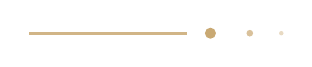
\begin{tikzpicture}
    \draw[GoldMain!60,line width=1.2pt] (0,0) -- (2.0,0);
    \fill[GoldMain!70] (2.3,0) circle (2pt);
    \fill[GoldMain!50] (2.8,0) circle (1.2pt);
    \fill[GoldMain!30] (3.2,0) circle (0.8pt);
  \end{tikzpicture}

  \vspace{0.8cm}

  % ── 主标题 ──
  {\Huge\bfseries\color{GreenDark} \@title\par}

  \vspace{0.6cm}
  % ── 英文副标题 ──
  {\Large\color{GreenMain!70} \@author\par}

  \vspace{0.4cm}
  % ── 第二道装饰金线（两端圆点）──
  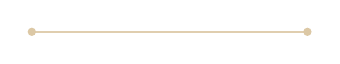
\begin{tikzpicture}
    \draw[GoldMain!40,line width=0.7pt] (0,0) -- (3.5,0);
    \fill[GoldMain!45] (0,0) circle (1.5pt);
    \fill[GoldMain!45] (3.5,0) circle (1.5pt);
  \end{tikzpicture}

  \vspace{0.8cm}
  % ── Fraktur 铭文 ──
  {\large\color{GoldMain!85} $\mathfrak{For}\quad\mathfrak{the}\quad\mathfrak{Worthy}$\par}

  \vspace{1.0cm}


\end{minipage}

% ============================================================
%  第七层：右下角「出版社」小 logo（仿 Springer 风格）
% ============================================================
\begin{tikzpicture}[remember picture, overlay]
  \begin{scope}[shift={([xshift=-5.5cm, yshift=1.5cm]current page.south east)}]
    % 小房子
    \draw[GreenMain, line width=0.8pt] (0,0) rectangle (0.9,0.72);
    \draw[GreenMain, line width=0.8pt] (0,0.72) -- (0.45,1.08) -- (0.9,0.72);
    \draw[GoldMain, line width=0.5pt] (0.45,0.72) -- (0.45,1.08);
    \draw[GreenMain, line width=0.4pt] (0.23,0) -- (0.23,0.72);
    \draw[GreenMain, line width=0.4pt] (0.67,0) -- (0.67,0.72);
    % 屋顶金点
    \fill[GoldMain] (0.45,1.08) circle (1.5pt);
    \node[anchor=west, GreenMain, font=\footnotesize] at (1.1,0.32)
      {Produced by Huginn};
  \end{scope}
\end{tikzpicture}

% ============================================================
%  第八层：底部主封面图片 —— 与金色框左右对齐，位于小房子上方
% ============================================================
\ifdefempty{\@coverimage}{}{
	\begin{tikzpicture}[remember picture,overlay]
		\node[
		anchor=south west,
		inner sep=0pt,
		outer sep=0pt
		] at ([xshift=3.3cm,yshift=3.05cm]current page.south west)
		{
			\includegraphics[
			width=\dimexpr\paperwidth-4.8cm\relax
			]{\@coverimage}
		};
	\end{tikzpicture}
}

% ============================================================
%  第九层：散落装饰点（页面随机分布的数学点缀）
% ============================================================
\begin{tikzpicture}[remember picture,overlay]
  % 右中区域散点
  \fill[GoldMain!20] ([xshift=-3.0cm,yshift=-9.5cm]current page.north west) circle (1.0pt);
  \fill[GreenAccent!20] ([xshift=-3.8cm,yshift=-9.8cm]current page.north west) circle (0.7pt);
  \fill[GoldMain!18] ([xshift=-2.5cm,yshift=-10.2cm]current page.north west) circle (0.8pt);
  % 右下方散点
  \fill[GreenMain!15] ([xshift=-4.0cm,yshift=3.5cm]current page.south west) circle (1.2pt);
  \fill[GoldMain!15] ([xshift=-5.5cm,yshift=4.0cm]current page.south west) circle (0.9pt);
  \fill[GreenAccent!12] ([xshift=-4.8cm,yshift=3.0cm]current page.south west) circle (0.6pt);
  % 标题区附近轻微装饰
  \fill[GoldMain!22] ([xshift=14.5cm,yshift=-6.0cm]current page.north west) circle (1.0pt);
  \fill[GreenAccent!18] ([xshift=14.0cm,yshift=-5.5cm]current page.north west) circle (0.6pt);
  \fill[GoldMain!18] ([xshift=15.0cm,yshift=-5.8cm]current page.north west) circle (0.8pt);
\end{tikzpicture}

\end{titlepage}
}
\makeatother

\addbibresource{bibliography/references.bib}

% ── 文档元信息与封面 ──
\title{概率论笔记}
\author{Notes on Probability Theory}
\date{\today}
\coverimage{figure/封面(1).jpg}

\begin{document}

\makecover

\frontmatter

\chapter*{前言}
\addcontentsline{toc}{chapter}{前言}


\begin{flushright}
	Huginn Wong\\
	\today
\end{flushright}

\tableofcontents
\newpage

\mainmatter
\setcounter{page}{1}

% ═══════════════════════════════════════════════════════
%  Part I：概率论基础
% ═══════════════════════════════════════════════════════
\setpartimage{}
\setpartintro{}
\part{概率论基础}

\setchapterimage{}
\setchapterintro{}
\setchapterimage{}
\setchapterintro{}
\chapter{概率空间与随机事件}

\section{随机试验和事件}
\label{sec:random-experiment-and-event}

\subsection*{随机试验、样本空间与事件}

在固定条件下必定出现唯一结果的现象称为确定性现象；在固定条件下可能出现两个或两个以上结果的现象称为随机现象。概率论与数理统计研究随机现象的数量规律。

\begin{mydefinition}{随机试验}{random-experiment}
在概率论中，将满足下列条件的试验称为随机试验，简称试验：
\begin{enumerate}
\item 试验进行前，无法确切知道一定会出现哪个结果；
\item 已知试验所有可能的结果；
\item 试验结束后，能够明确知道哪个试验结果出现。
\end{enumerate}
\end{mydefinition}

\begin{mydefinition}{样本点与样本空间}{sample-space}
\begin{enumerate}
\item 一个随机试验的任意一个可能结果称为一个\textbf{样本点}（sample），记为 $\omega$；
\item 该随机试验所有可能结果组成的集合称为该试验的\textbf{样本空间}（sample space），记为 $\Omega$。
\end{enumerate}
\end{mydefinition}

样本点和样本空间的关系为
\[
\omega\in\Omega.
\]
样本空间 $\Omega$ 可以是有限集、无限集，也可以是以函数为元素的集合。用集合语言描述试验结果具有抽象性和普遍性，便于刻画不同随机试验的共同结构。

\begin{mydefinition}{事件}{event}
\begin{enumerate}
\item 样本空间 $\Omega$ 的一个子集称为一个\textbf{事件}，通常用大写字母 $A,B,C,\ldots$ 表示；
\item 对事件 $A$，若试验结果 $\omega\in A$，则称事件 $A$ 发生；否则称事件 $A$ 不发生。
\end{enumerate}
\end{mydefinition}

\textbf{注:(基本事件)}样本空间 $\Omega$ 包含所有试验结果，故称为\textbf{必然事件}；空集 $\varnothing$ 不含任何样本点，故称为\textbf{不可能事件}。

下面用集合的关系与运算刻画事件的关系与运算。

\begin{enumerate}
\item \textbf{事件的包含与相等}

若 $A\subseteq B$，则称事件 $B$ 包含事件 $A$，或称事件 $A$ 包含在事件 $B$ 中。其概率意义是：若事件 $A$ 发生，则事件 $B$ 必发生。

若 $A\subseteq B$ 且 $B\subseteq A$，即 $A=B$，则称事件 $A$ 与事件 $B$ 相等；其概率意义是二者同时发生、同时不发生。

\item \textbf{事件的并}

集合 $A\cup B$ 称为事件 $A$ 与 $B$ 的并事件，其概率意义是 $A$ 与 $B$ 至少有一个发生。更一般地，
\[
\bigcup_{i=1}^{n} A_i
=\left\{\omega\in\Omega\mathrel{\big|}\exists\, i\in\{1,\ldots,n\},\ \omega\in A_i\right\},
\]
表示 $n$ 个事件中至少有一个发生；而
\[
\bigcup_{i=1}^{\infty} A_i
=\left\{\omega\in\Omega\mathrel{\big|}\exists\, i\geq 1,\ \omega\in A_i\right\},
\]
表示可数个事件中至少有一个发生。

\item \textbf{事件的交（积）}

集合 $A\cap B$ 称为事件 $A$ 与 $B$ 的交（积）事件，其概率意义是 $A$ 与 $B$ 都发生。类似地，
\[
\bigcap_{i=1}^{n} A_i
=\left\{\omega\in\Omega\mathrel{\big|}\forall\, i\in\{1,\ldots,n\},\ \omega\in A_i\right\},
\]
表示 $n$ 个事件都发生；
\[
\bigcap_{i=1}^{\infty} A_i
=\left\{\omega\in\Omega\mathrel{\big|}\forall\, i\geq 1,\ \omega\in A_i\right\},
\]
表示可数个事件都发生。为书写方便，常记 $AB:=A\cap B$。

\item \textbf{事件的差}

集合
\[
A\setminus B=\left\{\omega\in\Omega\mathrel{\big|}\omega\in A,\ \omega\notin B\right\}
\]
称为事件 $A$ 与 $B$ 的差，其概率意义是 $A$ 发生而 $B$ 不发生。

\item \textbf{互斥（互不相容）事件}

若 $A\cap B=\varnothing$，则称事件 $A$ 与 $B$ 互斥或互不相容，其概率意义是二者不能同时发生。若对一列事件 $A_n\ (n\geq1)$，任意 $i\ne j$ 都有 $A_i\cap A_j=\varnothing$，则称该列事件两两互斥。

\item \textbf{补事件}

事件 $A$ 的补集
\[
A^c=\left\{\omega\in\Omega\mathrel{\big|}\omega\notin A\right\}
\]
称为 $A$ 的补事件，其概率意义是 $A$ 不发生。并且
\[
A\setminus B=A\cap B^c.
\]
事件运算约定先进行补运算，再进行交运算，最后进行并运算或差运算。

\item \textbf{完备事件组}

若事件 $A_1,A_2,\ldots$ 两两互斥，且
\[
\bigcup_{i=1}^{\infty}A_i=\Omega,
\]
则称 $A_1,A_2,\ldots$ 构成一个\textbf{完备事件组}，或称为 $\Omega$ 的一个可数划分。
\end{enumerate}

事件的运算性质就是集合的运算性质。对任意事件 $A,B,C$，有
\[
A\cup B=B\cup A,\qquad A\cap B=B\cap A,
\]
\[
(A\cup B)\cup C=A\cup(B\cup C),\qquad
(A\cap B)\cap C=A\cap(B\cap C),
\]
\[
A\cup(B\cap C)=(A\cup B)\cap(A\cup C),\qquad
A\cap(B\cup C)=(A\cap B)\cup(A\cap C).
\]
此外，德摩根律为
\[
\left(\bigcup_{i=1}^{n}A_i\right)^c=\bigcap_{i=1}^{n}A_i^c,
\qquad
\left(\bigcap_{i=1}^{n}A_i\right)^c=\bigcup_{i=1}^{n}A_i^c,
\]
以及
\[
\left(\bigcup_{i=1}^{\infty}A_i\right)^c=\bigcap_{i=1}^{\infty}A_i^c,
\qquad
\left(\bigcap_{i=1}^{\infty}A_i\right)^c=\bigcup_{i=1}^{\infty}A_i^c.
\]

\subsection*{古典概率模型（高中内容）}

对事件 $A\subseteq\Omega$，用 $P(A)$ 表示事件 $A$ 发生的概率。

\begin{mydefinition}{古典概率模型}{classical-probability-model}
若某随机试验的样本空间 $\Omega$ 只含有限个样本点，且每个样本点出现的概率相等，则称该随机试验为\textbf{古典概率模型}，简称\textbf{古典概型}。对任意事件 $A\subseteq\Omega$，记 $A$ 中元素个数为 $n(A)$，则
\[
P(A)=\dfrac{n(A)}{n(\Omega)}.
\]
\end{mydefinition}

由古典概型的定义可知，计算 $P(A)$ 的关键在于计算 $n(A)$ 和 $n(\Omega)$，因此需要使用计数方法。

\begin{proposition}{计数的乘法原理}{multiplication-principle}
若一个过程由 $r$ 个试验构成，第 $i$ 个试验有 $n_i$ 种可能结果，则该过程共有
\[
n_1n_2\cdots n_r
\]
种可能结果。
\end{proposition}
\begin{example}
	\begin{enumerate}
		\item 有放回有序抽取：从 $n$ 个不同的球中有放回地每次抽取一个，依次抽取 $m$ 次并按顺序排成一列，可得到 $n^m$ 个不同排列。
		\item 无放回有序抽取：从 $n$ 个不同的球中无放回地抽取 $m$ 个并按顺序排成一列，可得到
		\[
		A_n^m=n(n-1)\cdots(n-m+1)=\dfrac{n!}{(n-m)!}
		\]
		个不同排列。
		\item 圆排列数：$n$个人坐一圈，有$(n-1)!$种排列方式.
		\item 组合数：从 $n$ 个不同的球中无放回地抽取 $m$ 个并放在一起，不计顺序，可得到
		\[
		C_n^m=\binom{n}{m}=\dfrac{n!}{(n-m)!m!}
		\]
		个不同组合。
	\end{enumerate}
\end{example}

\begin{proposition}{多组分配}{multinomial-count}
将 $n$ 个不同元素分成 $r$ 个组，其中第 $i$ 组有 $n_i$ 个元素，组内不计顺序，且
\[
n_1+n_2+\cdots+n_r=n,
\]
则不同分法共有
\[
\dfrac{n!}{n_1!n_2!\cdots n_r!}
\]
种。
\end{proposition}

\begin{proof}
依次选出各组元素，不同分法数为
\[
\binom{n}{n_1}
\binom{n-n_1}{n_2}
\binom{n-n_1-n_2}{n_3}
\cdots
\binom{n-n_1-\cdots-n_{r-1}}{n_r}.
\]
将各组合数相乘并约去中间阶乘，得到
\[
\dfrac{n!}{n_1!n_2!\cdots n_r!}.
\]
\end{proof}

\begin{mycorollary}{多项式定理}{multinomial-theorem}
\[
(x_1+x_2+\cdots+x_r)^n
=\sum_{n_1+n_2+\cdots+n_r=n}
\dfrac{n!}{n_1!n_2!\cdots n_r!}
x_1^{n_1}x_2^{n_2}\cdots x_r^{n_r}.
\]
其中
\[
\binom{n}{n_1,n_2,\ldots,n_r}
:=\dfrac{n!}{n_1!n_2!\cdots n_r!}
\]
称为多项式系数。
\end{mycorollary}
\newpage
\begin{proposition}{正整数解的个数}{positive-integer-solutions}
设 $n\geq1$，方程
\[
x_1+x_2+\cdots+x_r=n,\qquad x_i>0\quad(i=1,2,\ldots,r)
\]
有
\[
\binom{n-1}{r-1}
\]
个不同的正整数解。
\end{proposition}

\begin{proof}
将 $n$ 个 $0$ 排成一行，从其中的 $n-1$ 个间隔中选出 $r-1$ 个插入隔板。令 $x_1$ 为第一个隔板左侧 $0$ 的个数，$x_2$ 为前两个隔板之间 $0$ 的个数，依此类推，$x_r$ 为最后一个隔板右侧 $0$ 的个数。

每一种隔板插法恰对应方程的一个正整数解，故不同解的个数为
\[
\binom{n-1}{r-1}.
\]
\end{proof}

\begin{proposition}{非负整数解的个数}{nonnegative-integer-solutions}
设 $n\geq1$，方程
\[
x_1+x_2+\cdots+x_r=n,\qquad x_i\geq0\quad(i=1,2,\ldots,r)
\]
有
\[
\binom{n+r-1}{r-1}
\]
个不同的非负整数解。
\end{proposition}

\begin{proof}
令 $y_i=x_i+1\ (i=1,2,\ldots,r)$。则 $x_1,x_2,\ldots,x_r$ 为满足原方程的非负整数解，当且仅当 $y_1,y_2,\ldots,y_r$ 为满足
\[
y_1+y_2+\cdots+y_r=n+r,\qquad y_i>0
\]
的正整数解。由正整数解的个数公式，所求解数为
\[
\binom{n+r-1}{r-1}.
\]
\end{proof}

\subsection*{几何概率模型（高中内容）}

\begin{mydefinition}{几何概率模型}{geometric-probability-model}
设随机试验的样本空间 $\Omega$ 是 $\mathbb{R}^d$ 中一个具有体积 $m(\Omega)$ 的子集，且
\[
0<m(\Omega)<+\infty.
\]
若事件 $A\subseteq\Omega$ 具有体积 $m(A)$，并规定
\[
P(A)=\dfrac{m(A)}{m(\Omega)},
\]
则称该随机试验为\textbf{几何概率模型}，简称\textbf{几何概型}。
\end{mydefinition}

\textbf{注：}几何概型也是一种等可能模型：对具有相同体积（在平面上即相同面积）的事件，它们发生的可能性相同。

\vspace{2\baselineskip}

\begin{example}[贝特朗奇论]
随机地从半径为 $r$ 的圆中取一根弦，求该弦长度大于圆内接正三角形边长 $\sqrt{3}r$ 的概率。设事件 $A$ 表示“弦长大于 $\sqrt{3}r$”。

“随机取弦”的说法本身并未说明等可能的参照标准，因此可以得到不同的概率。
\begin{enumerate}
\item 若以弦的中点 $M$ 确定一根弦，并规定 $M$ 在大圆内均匀取值，则弦长大于 $\sqrt{3}r$ 当且仅当 $M$ 落在半径为 $r/2$ 的同心小圆内。因此
\[
P(A)=\dfrac{\pi(r/2)^2}{\pi r^2}=\dfrac14.
\]

\item 若固定弦的一个端点，并规定弦与该端点处切线的夹角 $\theta$ 在 $[0,\pi]$ 上均匀取值，则
\[
A=\left(\dfrac{\pi}{3},\dfrac{2\pi}{3}\right),
\qquad
P(A)=\dfrac{\pi/3}{\pi}=\dfrac13.
\]

\item 若以弦到圆心的距离 $D$ 确定一根弦，并规定 $D$ 在 $[0,r]$ 上均匀取值，则 $A=\{0<D<r/2\}$，从而
\[
P(A)=\dfrac{r/2}{r}=\dfrac12.
\]
\end{enumerate}

三种理解得到不同答案的原因在于：它们分别选择了不同的样本空间和等可能标准。求概率前，必须先明确随机试验的样本空间以及概率模型。
\end{example}

\begin{example}[布丰投针实验]
在平面上画出间距为 $d$ 的一组平行直线。随机投掷一根长度为 $l$ 的针，设
\[
0<l\leq d.
\]
记针与任一直线相交为事件 $A$。令 $X$ 表示针的中点到最近平行线的距离，$\Theta$ 表示针与平行线的夹角。按照几何概型，取
\[
0\leq X\leq \dfrac d2,
\qquad
0\leq \Theta\leq \dfrac{\pi}{2},
\]
并把 $(X,\Theta)$ 看作在该矩形内等可能取值。

针与直线相交当且仅当
\[
X\leq \dfrac l2\sin\Theta.
\]
因此，事件 $A$ 对应的面积为
\[
\int_0^{\pi/2}\dfrac l2\sin\theta\,\mathrm{d}\theta
=\dfrac l2,
\]
而样本空间的面积为 $\dfrac d2\cdot\dfrac{\pi}{2}=\dfrac{d\pi}{4}$。故
\[
P(A)=\dfrac{l/2}{d\pi/4}=\dfrac{2l}{\pi d}.
\]

若独立投针 $N$ 次，其中有 $H$ 次与直线相交，则当 $N$ 较大时，频率 $H/N$ 可近似看作 $P(A)$，从而得到 $\pi$ 的实验估计式
\[
\pi\approx\dfrac{2lN}{dH}.
\]
\end{example}

\vspace{2\baselineskip}

\section{可测空间和概率空间}

古典概型和几何概型都是等可能模型，但并非所有随机试验都能归结为这两类模型。贝特朗奇论还表明，必须用更严格的形式明确样本空间和概率的含义，才能避免由语义歧义带来的不同答案。

\subsection*{面积和频率}

设 $A\subseteq\mathbb{R}^d$，用 $\mu(A)$ 表示 $A$ 的面积、长度或体积。直观上，$\mu(\cdot)$ 具有下列性质：
\begin{enumerate}
\item $\mu(A)\geq0$；
\item $\mu(\varnothing)=0$；
\item 若 $A\subseteq B$，且 $0\leq\mu(A),\mu(B)<+\infty$，则
\[
\mu(B\setminus A)=\mu(B)-\mu(A);
\]
\item 若 $A_1,A_2,\ldots$ 两两互斥，则
\[
\mu\left(\bigcup_{n=1}^{\infty}A_n\right)
=\sum_{n=1}^{\infty}\mu(A_n).
\]
\end{enumerate}

日常生活中也常以频率描述事件发生的可能性。频率的性质将启发我们给出概率的公理化定义。

\begin{mydefinition}{频率}{frequency}
在 $N$ 次重复试验中，若事件 $A$ 出现 $N(A)$ 次，则比值
\[
f_N(A)=\dfrac{N(A)}{N}
\]
称为事件 $A$ 发生的\textbf{频率}。
\end{mydefinition}

\begin{proposition}{频率的性质}{frequency-properties}
对任意事件 $A$，有
\[
0\leq f_N(A)\leq1,
\qquad
f_N(\Omega)=1,
\qquad
f_N(\varnothing)=0.
\]
并且
\[
f_N(A^c)=1-f_N(A).
\]
若 $A_1,A_2,\ldots,A_r$ 两两互斥，则
\[
f_N\left(\bigcup_{i=1}^{r}A_i\right)
=\sum_{i=1}^{r}f_N(A_i).
\]
\end{proposition}

\begin{proof}
由 $0\leq N(A)\leq N$，两端除以 $N$ 即得 $0\leq f_N(A)\leq1$。每次试验中 $\Omega$ 都发生而 $\varnothing$ 都不发生，故 $N(\Omega)=N$、$N(\varnothing)=0$。

若 $A_1,\ldots,A_r$ 两两互斥，则每次试验至多落入其中一个事件，因此
\[
N\left(\bigcup_{i=1}^{r}A_i\right)=\sum_{i=1}^{r}N(A_i).
\]
两端除以 $N$ 即得结论。

又因为在每次试验中，$A$ 与 $A^c$ 恰有一个发生，故 $N(A^c)=N-N(A)$，从而
\[
f_N(A^c)=\dfrac{N-N(A)}{N}=1-f_N(A).
\]
\end{proof}

频率反映了事件在重复试验中发生的频繁程度，并直观地反映事件在一次试验中发生的可能性大小。

\subsection*{可测空间}

由面积和频率的性质可见，面积 $\mu(\cdot)$、频率 $f_N(\cdot)$ 以及概率 $P(\cdot)$ 都是以集合为自变量的函数。为了说明哪些子集可以作为事件，需要先规定一个对补集和可数并封闭的集合类。

\begin{mydefinition}{$\sigma$-域与可测空间}{sigma-algebra}
设 $\Omega$ 是非空集合，$\mathscr{F}$ 是由 $\Omega$ 的一些子集构成的集合类。若 $\mathscr{F}$ 满足：
\begin{enumerate}
\item $\Omega\in\mathscr{F}$；
\item 若 $A\in\mathscr{F}$，则 $A^c\in\mathscr{F}$；
\item 若 $A_n\in\mathscr{F}$（$n\geq1$），则
\[
\bigcup_{n=1}^{\infty}A_n\in\mathscr{F},
\]
\end{enumerate}
则称 $\mathscr{F}$ 为 $\Omega$ 的一个\textbf{$\sigma$-域}或\textbf{事件域}，在分析学中我们称之为\textbf{$\sigma$-代数}，$\mathscr{F}$ 中的元素称为事件或可测集，二元组 $(\Omega,\mathscr{F})$ 称为\textbf{可测空间}。
\end{mydefinition}

\begin{proposition}{$\sigma$-域的基本封闭性}{sigma-algebra-closure}
若 $\mathscr{F}$ 是 $\Omega$ 的一个 $\sigma$-域，则：
\begin{enumerate}
\item $\varnothing\in\mathscr{F}$；
\item 若 $A_n\in\mathscr{F}$（$n\geq1$），则
\[
\bigcap_{n=1}^{\infty}A_n\in\mathscr{F};
\]
\item 若 $A_1,\ldots,A_k\in\mathscr{F}$，则有限并与有限交都属于 $\mathscr{F}$；
\item 若 $A,B\in\mathscr{F}$，则 $A\setminus B\in\mathscr{F}$。
\end{enumerate}
\end{proposition}

\begin{proof}
由 $\Omega\in\mathscr{F}$ 及补集封闭性，得 $\varnothing=\Omega^c\in\mathscr{F}$。若 $A_n\in\mathscr{F}$，则 $A_n^c\in\mathscr{F}$，从而
\[
\bigcap_{n=1}^{\infty}A_n
=\left(\bigcup_{n=1}^{\infty}A_n^c\right)^c
\in\mathscr{F}.
\]
有限并可视为可数并中从第 $k+1$ 项起均取空集的情形；有限交由德摩根律得到。最后，$B^c\in\mathscr{F}$，故
\[
A\setminus B=A\cap B^c\in\mathscr{F}.
\]
\end{proof}

\begin{example}[一些 $\sigma$-代数的例子]
\begin{enumerate}
\item $\{\varnothing,\Omega\}$ 是 $\Omega$ 上所含事件最少的 $\sigma$-域；
\item 对任意 $A\subseteq\Omega$，集合类
\[
\{\varnothing,\Omega,A,A^c\}
\]
是包含 $A$ 的一个 最小的$\sigma$-域；
\item $\mathcal{P}(\Omega):=\{A\mid A\subseteq\Omega\}$ 是 $\Omega$ 的所有子集构成的 $\sigma$-域。
\end{enumerate}
\end{example}

\textbf{注：}样本点 $\omega\in\Omega$ 并不必然意味着单点集 $\{\omega\}$ 属于 $\mathscr{F}$。因此，只有在固定可测空间 $(\Omega,\mathscr{F})$ 后，才能判断某个子集是否为事件。

\begin{proposition}{$\sigma$-域的交}{intersection-of-sigma-algebras}
设 $I$ 是一个指标集。若对任意 $\alpha\in I$，$\mathscr{F}_\alpha$ 都是 $\Omega$ 上的 $\sigma$-域，则
\[
\mathscr{F}=\bigcap_{\alpha\in I}\mathscr{F}_\alpha
\]
也是 $\Omega$ 上的 $\sigma$-域。
\end{proposition}

\begin{proof}
对每个 $\alpha\in I$，都有 $\Omega\in\mathscr{F}_\alpha$，故 $\Omega\in\mathscr{F}$。若 $A\in\mathscr{F}$，则 $A\in\mathscr{F}_\alpha$ 对所有 $\alpha\in I$ 成立，因而 $A^c\in\mathscr{F}_\alpha$ 对所有 $\alpha$ 成立，即 $A^c\in\mathscr{F}$。同理，若 $A_n\in\mathscr{F}$（$n\geq1$），则 $\bigcup_{n=1}^{\infty}A_n\in\mathscr{F}_\alpha$ 对所有 $\alpha$ 成立，故该可数并属于 $\mathscr{F}$。
\end{proof}

\begin{mytheorem}{由集合类生成的 $\sigma$-域}{generated-sigma-algebra}
设 $\Omega$ 是非空集合，$\mathscr{E}$ 是由 $\Omega$ 的一些子集构成的非空集合类。则存在唯一的 $\sigma$-域 $\mathscr{F}$ 满足：
\begin{enumerate}
\item $\mathscr{E}\subseteq\mathscr{F}$；
\item 对任意包含 $\mathscr{E}$ 的 $\sigma$-域 $\mathcal{M}$，都有 $\mathscr{F}\subseteq\mathcal{M}$。
\end{enumerate}
此时称 $\mathscr{F}$ 为由 $\mathscr{E}$ \textbf{生成的 $\sigma$-域}，记为 $\sigma(\mathscr{E})$。
\end{mytheorem}

\begin{proof}
令
\[
\mathscr{F}
=\bigcap_{\substack{\mathscr{M}\text{ 是 }\Omega\text{ 上的 }\sigma\text{-域}\\ \mathscr{E}\subseteq\mathscr{M}}}\mathscr{M}.
\]
因为 $\mathcal{P}(\Omega)$ 是包含 $\mathscr{E}$ 的 $\sigma$-域，故上式中的交非空。由上一命题，$\mathscr{F}$ 是 $\sigma$-域；由定义，$\mathscr{E}\subseteq\mathscr{F}$，并且 $\mathscr{F}$ 包含于任意包含 $\mathscr{E}$ 的 $\sigma$-域。唯一性由这一最小性立刻得到。
\end{proof}

\begin{mydefinition}{Borel $\sigma$-域}{borel-sigma-algebra}
记
\[
\mathscr{E}_{\mathbb{R}}=\{(a,b]\mid a,b\in\mathbb{R}\}.
\]
称 $\sigma(\mathscr{E}_{\mathbb{R}})$ 为 $\mathbb{R}$ 上的\textbf{Borel $\sigma$-域}，记为 $\mathscr{B}(\mathbb{R})$。

类似地，记
\[
\mathscr{E}_{\mathbb{R}^d}
=\left\{(a_1,b_1]\times\cdots\times(a_d,b_d]\mid a_i,b_i\in\mathbb{R},\ 1\leq i\leq d\right\}.
\]
称 $\sigma(\mathscr{E}_{\mathbb{R}^d})$ 为 $\mathbb{R}^d$ 上的 Borel $\sigma$-域，记为 $\mathscr{B}(\mathbb{R}^d)$。
\end{mydefinition}

\begin{proposition}{常用集合属于 $\mathscr{B}(\mathbb{R})$}{common-borel-sets}
对任意 $a<b$，开区间 $(a,b)$、闭区间 $[a,b]$、半开半闭区间 $[a,b)$ 以及单点集 $\{b\}$ 都属于 $\mathscr{B}(\mathbb{R})$。
\end{proposition}

\begin{proof}
对任意 $k\geq1$，$(a,b-1/k]\in\mathscr{B}(\mathbb{R})$。于是
\[
(a,b)=\bigcup_{k=1}^{\infty}(a,b-1/k]\in\mathscr{B}(\mathbb{R}).
\]
由差集封闭性，
\[
\{b\}=(a,b]\setminus(a,b)\in\mathscr{B}(\mathbb{R}).
\]
同理 $\{a\}\in\mathscr{B}(\mathbb{R})$，再由有限并封闭性可得
\[
[a,b]=(a,b]\cup\{a\},
\qquad
[a,b)=(a,b)\cup\{a\}
\]
均属于 $\mathscr{B}(\mathbb{R})$。
\end{proof}

\subsection*{概率的公理化定义和性质}

概率的公理化定义继承了频率的非负性、规范性和可加性。

\begin{mydefinition}{概率与概率空间}{probability-space}
设 $\Omega$ 是非空集合，$\mathscr{F}$ 是 $\Omega$ 上给定的一个 $\sigma$-域。若映射
\[
P:\mathscr{F}\longrightarrow[0,+\infty)
\]
满足：
\begin{enumerate}
\item \textbf{非负性：}对任意 $A\in\mathscr{F}$，有 $P(A)\geq0$；
\item \textbf{规范性：}$P(\Omega)=1$；
\item \textbf{可列可加性：}若 $A_n\in\mathscr{F}$（$n\geq1$）两两互斥，则
\[
P\left(\bigcup_{n=1}^{\infty}A_n\right)
=\sum_{n=1}^{\infty}P(A_n),
\]
\end{enumerate}
则称 $P$ 为 $\mathscr{F}$ 上的\textbf{概率}，三元组 $(\Omega,\mathscr{F},P)$ 称为\textbf{概率空间}。
\end{mydefinition}
可以看到的是，$P$实际上就是一个测度，概率空间$(\Omega,\mathscr{F},P)$是一个测度空间.
\subsection*{概率的性质}
\begin{proposition}{空集的概率}{probability-empty-set}
\[
P(\varnothing)=0.
\]
\end{proposition}

\begin{proof}
令 $A_1=\Omega$，$A_n=\varnothing$（$n\geq2$）。则 $A_1,A_2,\ldots$ 两两互斥，且其并为 $\Omega$。由规范性和可列可加性，
\[
1=P(\Omega)=\sum_{n=1}^{\infty}P(A_n)
=P(\Omega)+\sum_{n=2}^{\infty}P(\varnothing).
\]
若 $P(\varnothing)>0$，右端将大于 $1$，矛盾，故 $P(\varnothing)=0$。
\end{proof}

\textbf{注：}当 $A=\varnothing$ 时，必有 $P(A)=0$；反过来，$P(A)=0$ 并不能推出 $A=\varnothing$。例如在几何概型 $\Omega=[0,1]$ 中，单点集 $\{a\}$（$a\in[0,1]$）满足
\[
P(\{a\})=\dfrac{m(\{a\})}{m(\Omega)}=0,
\]
但 $\{a\}$ 不是空集。满足 $P(A)=0$ 的事件称为\textbf{零概率集}。

\begin{proposition}{有限可加性}{finite-additivity}
若 $A_1,\ldots,A_n\in\mathscr{F}$ 两两互斥，则
\[
P\left(\bigcup_{i=1}^{n}A_i\right)
=\sum_{i=1}^{n}P(A_i).
\]
\end{proposition}

\begin{proof}
令 $A_{n+k}=\varnothing$（$k\geq1$），将有限个事件补成可列个两两互斥事件。由可列可加性及 $P(\varnothing)=0$，即得结论。
\end{proof}

\begin{proposition}{单调性}{probability-monotonicity}
若 $A,B\in\mathscr{F}$ 且 $B\subseteq A$，则
\[
P(B)\leq P(A).
\]
\end{proposition}

\begin{proof}
因为 $A=B\cup(A\setminus B)$，且两部分互斥，故
\[
P(A)=P(B)+P(A\setminus B)\geq P(B).
\]
\end{proof}

\begin{mycorollary}{概率的上界}{probability-upper-bound}
对任意 $A\in\mathscr{F}$，有
\[
0\leq P(A)\leq1.
\]
\end{mycorollary}

\begin{proof}
左侧由非负性成立；又 $A\subseteq\Omega$，故由单调性和规范性，$P(A)\leq P(\Omega)=1$。
\end{proof}

\begin{proposition}{补事件的概率}{probability-complement}
对任意 $A\in\mathscr{F}$，有
\[
P(A^c)=1-P(A).
\]
\end{proposition}

\begin{proof}
由于 $A\cap A^c=\varnothing$ 且 $A\cup A^c=\Omega$，由有限可加性得
\[
P(A)+P(A^c)=P(\Omega)=1.
\]
\end{proof}

\begin{proposition}{一般加法公式}{probability-addition-formula}
对任意事件 $A,B\in\mathscr{F}$，有
\[
P(A\cup B)=P(A)+P(B)-P(A\cap B).
\]
\end{proposition}

\begin{proof}
因为 $A\cup B=A\cup(B\setminus A)$，且 $A$ 与 $B\setminus A$ 互斥，故
\[
P(A\cup B)=P(A)+P(B\setminus A).
\]
又 $B=(B\setminus A)\cup(A\cap B)$ 为互斥并，故
\[
P(B\setminus A)=P(B)-P(A\cap B).
\]
代入即得结论。
\end{proof}

\textbf{注：}三个事件 $A,B,C$ 的一般加法公式为
\[
\begin{aligned}
P(A\cup B\cup C)={}&P(A)+P(B)+P(C)\\
&-P(A\cap B)-P(A\cap C)-P(B\cap C)\\
&+P(A\cap B\cap C).
\end{aligned}
\]

\begin{mytheorem}{容斥恒等式}{inclusion-exclusion}
对任意 $n$ 个事件 $A_1,A_2,\ldots,A_n$，有
\[
P\left(\bigcup_{i=1}^{n}A_i\right)
=\sum_{r=1}^{n}(-1)^{r+1}
\sum_{1\leq i_1<\cdots<i_r\leq n}
P\left(A_{i_1}\cap\cdots\cap A_{i_r}\right).
\]
\end{mytheorem}

\begin{proof}
对 $n$ 归纳。$n=1$ 时结论显然成立。设结论对 $n-1$ 个事件成立，令 $U_{n-1}=\bigcup_{i=1}^{n-1}A_i$。由一般加法公式，
\[
P(U_{n-1}\cup A_n)=P(U_{n-1})+P(A_n)-P(U_{n-1}\cap A_n).
\]
又
\[
U_{n-1}\cap A_n=\bigcup_{i=1}^{n-1}(A_i\cap A_n).
\]
分别对 $U_{n-1}$ 与右侧这个 $n-1$ 个事件的并使用归纳假设，合并不含 $A_n$ 和含 $A_n$ 的各项，便得到 $n$ 个事件的公式。
\end{proof}

\begin{mycorollary}{有限次次可加性}{finite-subadditivity}
对任意 $n$ 个事件 $A_1,\ldots,A_n$，有
\[
P\left(\bigcup_{i=1}^{n}A_i\right)
\leq\sum_{i=1}^{n}P(A_i).
\]
\end{mycorollary}

\begin{proof}
对 $n$ 归纳。$n=1$ 时结论显然成立。若结论对 $n-1$ 个事件成立，则由一般加法公式和 $P\bigl((\bigcup_{i=1}^{n-1}A_i)\cap A_n\bigr)\geq0$，有
\[
\begin{aligned}
P\left(\bigcup_{i=1}^{n}A_i\right)
&\leq P\left(\bigcup_{i=1}^{n-1}A_i\right)+P(A_n)\\
&\leq\sum_{i=1}^{n}P(A_i).
\end{aligned}
\]
\end{proof}

\begin{example}[Kounias 不等式]
对任意 $n$ 个事件 $A_1,\ldots,A_n$，有
\[
P\left(\bigcup_{r=1}^{n}A_r\right)
\leq\min_{1\leq k\leq n}
\left\{
\sum_{r=1}^{n}P(A_r)-\sum_{\substack{1\leq r\leq n\\ r\ne k}}P(A_r\cap A_k)
\right\}.
\]
\end{example}

\begin{proof}
固定 $k$。由有限次次可加性，
\[
\begin{aligned}
\sum_{r=1}^{n}P(A_r)-\sum_{r\ne k}P(A_r\cap A_k)
&=P(A_k)+\sum_{r\ne k}P(A_r\cap A_k^c)\\
&\geq P\left(A_k\cup\bigcup_{r\ne k}(A_r\cap A_k^c)\right)\\
&=P\left(\bigcup_{r=1}^{n}A_r\right).
\end{aligned}
\]
对 $k=1,\ldots,n$ 取最小值即得结论。
\end{proof}

\begin{mydefinition}{事件序列的极限}{limit-of-event-sequences}
若事件列 $\{A_n\}_{n\geq1}$ 满足
\[
A_1\subseteq A_2\subseteq\cdots\subseteq A_n\subseteq\cdots,
\]
则称其为\textbf{递增序列}（或不降序列），并定义
\[
\lim_{n\to\infty}A_n:=\bigcup_{n=1}^{\infty}A_n.
\]
若
\[
A_1\supseteq A_2\supseteq\cdots\supseteq A_n\supseteq\cdots,
\]
则称其为\textbf{递减序列}（或不增序列），并定义
\[
\lim_{n\to\infty}A_n:=\bigcap_{n=1}^{\infty}A_n.
\]
\end{mydefinition}

\begin{mytheorem}{概率的连续性}{continuity-of-probability}
\begin{enumerate}
\item 若 $\{A_n\}_{n\geq1}$ 为递增序列，则
\[
P\left(\lim_{n\to\infty}A_n\right)=\lim_{n\to\infty}P(A_n).
\]
称为概率的\textbf{下连续性}；
\item 若 $\{A_n\}_{n\geq1}$ 为递减序列，则
\[
P\left(\lim_{n\to\infty}A_n\right)=\lim_{n\to\infty}P(A_n).
\]
称为概率的\textbf{上连续性}。
\end{enumerate}
\end{mytheorem}

\begin{proof}
对递增序列，令 $F_1=A_1$，$F_n=A_n\setminus A_{n-1}$（$n\geq2$）。则 $F_1,F_2,\ldots$ 两两互斥，且
\[
\bigcup_{i=1}^{n}F_i=A_n,
\qquad
\bigcup_{i=1}^{\infty}F_i=\bigcup_{i=1}^{\infty}A_i.
\]
因此
\[
P\left(\lim_{n\to\infty}A_n\right)
=\sum_{i=1}^{\infty}P(F_i)
=\lim_{n\to\infty}\sum_{i=1}^{n}P(F_i)
=\lim_{n\to\infty}P(A_n).
\]
对递减序列，$\{A_n^c\}_{n\geq1}$ 为递增序列。由补事件公式和已证的下连续性，
\[
\begin{aligned}
P\left(\bigcap_{n=1}^{\infty}A_n\right)
&=1-P\left(\bigcup_{n=1}^{\infty}A_n^c\right)\\
&=1-\lim_{n\to\infty}P(A_n^c)
=\lim_{n\to\infty}P(A_n).
\end{aligned}
\]
\end{proof}

\begin{proposition}{可列次可加性（布尔不等式）}{countable-subadditivity}
对任意可列个事件 $A_1,A_2,\ldots$，有
\[
P\left(\bigcup_{i=1}^{\infty}A_i\right)
\leq\sum_{i=1}^{\infty}P(A_i).
\]
\end{proposition}

\begin{proof}
令 $B_n=\bigcup_{i=1}^{n}A_i$。则 $\{B_n\}$ 为递增序列，且
\[
\lim_{n\to\infty}B_n=\bigcup_{i=1}^{\infty}A_i.
\]
由下连续性和有限次次可加性，
\[
\begin{aligned}
P\left(\bigcup_{i=1}^{\infty}A_i\right)
&=\lim_{n\to\infty}P(B_n)\\
&\leq\lim_{n\to\infty}\sum_{i=1}^{n}P(A_i)
=\sum_{i=1}^{\infty}P(A_i).
\end{aligned}
\]
\end{proof}

\begin{example}[可列个零概率事件的并]
若事件列 $\{A_i\}_{i\geq1}$ 满足 $P(A_i)=0$（$i\geq1$），则
\[
P\left(\bigcup_{i=1}^{\infty}A_i\right)=0.
\]
\end{example}

\begin{proof}
由布尔不等式，
\[
0\leq P\left(\bigcup_{i=1}^{\infty}A_i\right)
\leq\sum_{i=1}^{\infty}P(A_i)=0.
\]
\end{proof}

\textbf{注：}若事件列 $\{A_i\}_{i\geq1}$ 满足 $P(A_i)=1$（$i\geq1$），则 $P(A_i^c)=0$。因此
\[
P\left(\bigcap_{i=1}^{\infty}A_i\right)
=1-P\left(\bigcup_{i=1}^{\infty}A_i^c\right)=1.
\]

\begin{mydefinition}{事件列的上极限与下极限}{limsup-liminf-events}
设 $A_n\in\mathscr{F}$（$n\geq1$），不要求事件列 $\{A_n\}$ 单调。定义
\[
\limsup_{n\to\infty}A_n
:=\bigcap_{n=1}^{\infty}\bigcup_{k=n}^{\infty}A_k
\]
为事件列的\textbf{上极限}，定义
\[
\liminf_{n\to\infty}A_n
:=\bigcup_{n=1}^{\infty}\bigcap_{k=n}^{\infty}A_k
\]
为事件列的\textbf{下极限}。
\end{mydefinition}

\textbf{注：}对任意样本点 $\omega$，有
\[
\begin{aligned}
\limsup_{n\to\infty}A_n\text{发生}&\iff\omega\in\limsup_{n\to\infty}A_n\\&\iff \omega\in \bigcap_{n=1}^{\infty}\bigcup_{k=n}^{\infty}A_k,\\
&\iff \forall n\geqslant 1,\omega \in \bigcup_{k=n}^{\infty}A_k\\&\iff \forall n\geqslant 1,\exists k_n\geqslant n ,\text{使得}\omega\in A_{k_n}\\
&\iff \text{存在无穷子序列}A_{k_n}, k_n\geqslant n,\text{使得},\omega \in A_{k_n}\\
& \iff \text{存在无穷多个事件}A_{k_n},k_n\geqslant 1,\text{发生}
\end{aligned}
\]
\[
\begin{aligned}
	\liminf_{n\to\infty}A_n\text{发生}&\iff\omega\in\liminf_{n\to\infty}A_n\\&\iff \omega\in \bigcup_{n=1}^{\infty}\bigcap_{k=n}^{\infty}A_k,\\
	&\iff \exists n\geqslant 1,\omega \in \bigcap_{k=n}^{\infty}A_k\\&\iff \exists n\geqslant 1,\text{使得}\forall k\geqslant n ,\text{有}\omega\in A_{k}\\
	&\iff\exists n\geqslant 1,\text{使得}\forall k\geqslant n ,\text{有}A_{k}\text{发生}\\
	& \iff \text{最多只有有限个时间}A_k\text{不发生}
\end{aligned}
\]
因此，上极限表示“无穷多个 $A_n$ 发生”，下极限表示“只有有限个 $A_n$ 不发生”，并且恒有
\[
\liminf_{n\to\infty}A_n\subseteq\limsup_{n\to\infty}A_n.
\]
对于一般的事件列的极限，我们可以利用上下极限给出定义。
\begin{mydefinition}
	当一个事件列的上极限与下极限相等时，也即
	\[\liminf_{n\to\infty}A_n =\limsup_{n\to\infty}A_n\]
	时，我们定义这个事件列的极限为
	\[\lim\limits_{n\to\infty}A_n :=\liminf_{n\to\infty}A_n =\limsup_{n\to\infty}A_n\]
\end{mydefinition}
\subsection*{一些概率空间的例子和计算}

\begin{example}[伯努利概率空间]
设 $\Omega$ 是非空集合，$\varnothing\subsetneq A\subsetneq\Omega$，并令
\[
\mathscr{F}=\{\varnothing,\Omega,A,A^c\}.
\]
给定 $0<p<1$，定义
\[
P(\varnothing)=0,\qquad P(\Omega)=1,
\qquad P(A)=p,\qquad P(A^c)=1-p.
\]
则 $(\Omega,\mathscr{F},P)$ 构成一个概率空间，称为\textbf{伯努利概率空间}（或伯努利概率模型），它用于讨论单个事件是否发生。
\end{example}

\begin{example}[古典概率空间]
设 $\Omega$ 只含有限个样本点，并取
\[
\mathscr{F}=2^\Omega=\{A:A\subseteq\Omega\}.
\]
若 $n(A)$ 表示集合 $A$ 中元素的个数，定义
\[
P(A)=\frac{n(A)}{n(\Omega)},\qquad A\in\mathscr{F},
\]
则 $(\Omega,\mathscr{F},P)$ 构成古典概率空间。这里每个单点事件的概率均为 $1/n(\Omega)$。
\end{example}

\textbf{注：}计算古典概型时，可以不逐项写出样本空间和 $\sigma$-域，但必须先确认样本空间中的各单点事件等可能。

\begin{example}[最大号码问题]
某城市有编号为 $1,2,\ldots,N$ 的 $N$ 部卡车。独立记录遇到的 $n$ 辆卡车的编号，允许重复。求记录到的最大编号为 $k$（$1\leq k\leq N$）的概率。
\end{example}

\begin{proof}
令 $B_k$ 表示最大编号恰为 $k$，$A_k$ 表示最大编号不超过 $k$。则
\[
B_1=A_1,\qquad B_k=A_k\setminus A_{k-1}\quad(2\leq k\leq N),
\]
且
\[
P(A_k)=\left(\frac{k}{N}\right)^n.
\]
因此
\[
P(B_1)=\frac{1}{N^n},
\]
而当 $2\leq k\leq N$ 时，
\[
P(B_k)=P(A_k)-P(A_{k-1})
=\frac{k^n-(k-1)^n}{N^n}.
\]

\end{proof}

\begin{example}[配对问题]
在有 $n$ 人参加的晚会上，每人带来一顶各不相同的帽子。离场时，每人从随机混放的帽子中抽取一顶。求至少有一人抽到自己帽子的概率。
\end{example}

\begin{proof}
给人和帽子分别编号 $1,2,\ldots,n$，令 $A_i$ 表示第 $i$ 人抽到自己的帽子。对任意
$1\leq i_1<i_2<\cdots<i_r\leq n$，有
\[
P(A_{i_1}\cap\cdots\cap A_{i_r})=\frac{(n-r)!}{n!}.
\]
同阶交事件共有 $\binom{n}{r}$ 个，故
\[
\sum_{1\leq i_1<\cdots<i_r\leq n}
P(A_{i_1}\cap\cdots\cap A_{i_r})
=\binom{n}{r}\frac{(n-r)!}{n!}=\frac{1}{r!}.
\]
由容斥恒等式，所求概率为
\[
P\left(\bigcup_{i=1}^{n}A_i\right)
=\sum_{r=1}^{n}\frac{(-1)^{r+1}}{r!}
=1-\sum_{r=0}^{n}\frac{(-1)^r}{r!}.
\]
因此
\[
\lim_{n\to\infty}P\left(\bigcup_{i=1}^{n}A_i\right)
=1-e^{-1}\approx0.6321,
\]
而无人抽到自己帽子的概率趋于 $e^{-1}\approx0.3679$。
\end{proof}

\begin{example}[圆桌夫妻问题]
十对夫妻随机地沿圆桌坐下，求没有妻子坐在丈夫身边的概率。
\end{example}

\begin{proof}
令 $A_i$ 表示第 $i$ 对夫妻相邻（$i=1,2,\ldots,10$）。总坐法数为
$(20-1)!=19!$。指定 $r$ 对夫妻相邻时，将每对夫妻看作一个整体，并计入夫妻内部的两种次序，故
\[
P(A_{i_1}\cap\cdots\cap A_{i_r})
=\frac{2^r(20-r-1)!}{19!}
=\frac{2^r(19-r)!}{19!}.
\]
由容斥恒等式，至少有一对夫妻相邻的概率为
\[
P\left(\bigcup_{i=1}^{10}A_i\right)
=\sum_{r=1}^{10}(-1)^{r+1}\binom{10}{r}
\frac{2^r(19-r)!}{19!}
\approx0.6605.
\]
所以，没有夫妻相邻的概率约为
\[
1-0.6605=0.3395.
\]
\end{proof}

\begin{example}[反复抽取扑克牌中的大王]
从一副 $54$ 张的扑克牌中反复抽牌，每次抽取一张，记录后放回。求：
\begin{enumerate}
\item 一直抽不到大王的概率；
\item 无穷多次抽到大王的概率。
\end{enumerate}
\end{example}

\begin{proof}
设 $E_n$ 表示第 $n$ 次抽到大王。

对第一个问题，令
\[
C_n=\bigcap_{k=1}^{n}E_k^c.
\]
则 $C_n$ 表示前 $n$ 次均未抽到大王，且 $\{C_n\}$ 为递减序列。令
\[
C=\bigcap_{n=1}^{\infty}C_n,
\]
则 $C$ 表示始终抽不到大王。由独立性和概率的上连续性，
\[
P(C)=\lim_{n\to\infty}P(C_n)
=\lim_{n\to\infty}\left(\frac{53}{54}\right)^n=0.
\]
因此，最终至少抽到一次大王的概率为 $1$。

对第二个问题，令 $B$ 表示无穷多次抽到大王，则
\[
B=\limsup_{n\to\infty}E_n
=\bigcap_{n=1}^{\infty}\bigcup_{k=n}^{\infty}E_k.
\]
再令
\[
B_n=\bigcup_{k=n}^{\infty}E_k.
\]
事件 $B_n$ 表示“从第 $n$ 次抽牌起至少抽到一次大王”。由第一个问题同样的计算，
$P(B_n^c)=0$，故 $P(B_n)=1$。由于 $\{B_n\}$ 为递减序列，
\[
P(B)=P\left(\bigcap_{n=1}^{\infty}B_n\right)
=\lim_{n\to\infty}P(B_n)=1.
\]
\end{proof}

\textbf{注：}本例中“最终抽到大王”和“无穷多次抽到大王”的概率均为 $1$，但“概率为 $1$”并不等同于逻辑上的必然发生。把概率小于 $0.05$ 的事件称为“小概率事件”也是常见约定，而不是普遍的数学定义。

\subsection*{测度及其基本性质}

概率可以看作总质量为 $1$ 的测度。先将概率公理中的“规范性”放宽，即得到更一般的测度概念。

\begin{mydefinition}{测度、有限测度与 $\sigma$ 有限测度}{measure-space}
设 $\Omega$ 是非空集合，$\mathscr{F}$ 是 $\Omega$ 上给定的一个 $\sigma$-域。若映射
\[
\mu:\mathscr{F}\longrightarrow[0,+\infty]
\]
满足：
\begin{enumerate}
\item $\mu(\varnothing)=0$；
\item 对任意两两互斥的事件列 $A_1,A_2,\ldots\in\mathscr{F}$，有
\[
\mu\left(\bigcup_{n=1}^{\infty}A_n\right)
=\sum_{n=1}^{\infty}\mu(A_n),
\]
\end{enumerate}
则称 $\mu$ 为 $\mathscr{F}$ 上的\textbf{测度}，三元组 $(\Omega,\mathscr{F},\mu)$ 称为\textbf{测度空间}。

\end{mydefinition}
若存在两两互斥的事件列 $A_1,A_2,\ldots\in\mathscr{F}$，使得
\[
\bigcup_{n=1}^{\infty}A_n=\Omega,
\qquad
\mu(A_n)<+\infty\quad(n\geq1),
\]
则称 $\mu$ 为\textbf{$\sigma$ 有限测度}。若 $\mu(\Omega)<+\infty$，则称 $\mu$ 为\textbf{有限测度}；若 $\mu(\Omega)=1$，则称 $\mu$ 为\textbf{概率测度}，也简称为\textbf{概率}。
\textbf{注：}当 $\mu(\Omega)=1$ 时，上述定义恰好就是前面概率 $P$ 的公理化定义。因此，每个概率空间都是测度空间。

\begin{proposition}{测度的有限可加性}{measure-finite-additivity}
若 $A_1,\ldots,A_n\in\mathscr{F}$ 两两互斥，则
\[
\mu\left(\bigcup_{i=1}^{n}A_i\right)=\sum_{i=1}^{n}\mu(A_i).
\]
\end{proposition}

\begin{proof}
令 $A_{n+k}=\varnothing$（$k\geq1$），再对事件列 $A_1,A_2,\ldots$ 使用测度的可列可加性即可。
\end{proof}

\begin{proposition}{测度的单调性}{measure-monotonicity}
若 $A,B\in\mathscr{F}$ 且 $B\subseteq A$，则
\[
\mu(B)\leq\mu(A).
\]
\end{proposition}

\begin{proof}
由 $A=B\cup(A\setminus B)$，且右端两事件互斥，得
\[
\mu(A)=\mu(B)+\mu(A\setminus B)\geq\mu(B).
\]
\end{proof}

\begin{proposition}{测度的可减性}{measure-subtractivity}
若 $A,B\in\mathscr{F}$，$A\subseteq B$，且 $\mu(A)<+\infty$，则
\[
\mu(B\setminus A)=\mu(B)-\mu(A).
\]
\end{proposition}

\begin{proof}
由 $B=A\cup(B\setminus A)$，且右端两事件互斥，故
\[
\mu(B)=\mu(A)+\mu(B\setminus A).
\]
由于 $\mu(A)<+\infty$，可移项得到结论。
\end{proof}

\begin{proposition}{测度的容斥恒等式}{measure-inclusion-exclusion}
若 $A_1,A_2,\ldots,A_n\in\mathscr{F}$，且对每个 $1\leq k\leq n$ 都有 $\mu(A_k)<+\infty$，则
\[
\mu\left(\bigcup_{k=1}^{n}A_k\right)
=\sum_{r=1}^{n}(-1)^{r+1}
\sum_{1\leq i_1<i_2<\cdots<i_r\leq n}
\mu(A_{i_1}\cap A_{i_2}\cap\cdots\cap A_{i_r}).
\]
\end{proposition}

\begin{proof}
将概率容斥公式的证明中 $P$ 全部替换为 $\mu$ 即可；有限性条件保证各项的减法有意义。
\end{proof}

\begin{mytheorem}{测度的可列次可加性}{measure-countable-subadditivity}
对任意事件列 $A_1,A_2,\ldots\in\mathscr{F}$，有
\[
\mu\left(\bigcup_{n=1}^{\infty}A_n\right)
\leq\sum_{n=1}^{\infty}\mu(A_n).
\]
\end{mytheorem}

\begin{proof}
令 $B_1=A_1$，并对 $n\geq2$ 令
\[
B_n=A_n\setminus\bigcup_{k=1}^{n-1}A_k.
\]
则 $B_1,B_2,\ldots$ 两两互斥，$B_n\subseteq A_n$，且
\[
\bigcup_{n=1}^{\infty}A_n=\bigcup_{n=1}^{\infty}B_n.
\]
故由可列可加性和单调性，
\[
\mu\left(\bigcup_{n=1}^{\infty}A_n\right)
=\sum_{n=1}^{\infty}\mu(B_n)
\leq\sum_{n=1}^{\infty}\mu(A_n).
\]
\end{proof}

\begin{proposition}{测度的下连续性}{measure-lower-continuity}
若 $\{A_n\}_{n\geq1}\subseteq\mathscr{F}$ 为递增序列，则
\[
\mu\left(\lim_{n\to\infty}A_n\right)
=\lim_{n\to\infty}\mu(A_n).
\]
\end{proposition}

\begin{proof}
令 $F_1=A_1$，$F_n=A_n\setminus A_{n-1}$（$n\geq2$）。仿照概率下连续性的证明，对两两互斥的 $F_n$ 应用测度的可列可加性即可。
\end{proof}

\begin{proposition}{测度的上连续性}{measure-upper-continuity}
若 $\{A_n\}_{n\geq1}\subseteq\mathscr{F}$ 为递减序列，且 $\mu(A_1)<+\infty$，则
\[
\mu\left(\lim_{n\to\infty}A_n\right)
=\lim_{n\to\infty}\mu(A_n).
\]
\end{proposition}

\begin{proof}
令 $C_n=A_1\setminus A_n$。则 $\{C_n\}$ 为递增序列，且
\[
\bigcup_{n=1}^{\infty}C_n
=A_1\setminus\bigcap_{n=1}^{\infty}A_n.
\]
由下连续性和可减性，
\[
\begin{aligned}
\mu(A_1)-\mu\left(\bigcap_{n=1}^{\infty}A_n\right)
&=\mu\left(\bigcup_{n=1}^{\infty}C_n\right)\\
&=\lim_{n\to\infty}\mu(C_n)\\
&=\lim_{n\to\infty}\bigl[\mu(A_1)-\mu(A_n)\bigr].
\end{aligned}
\]
由于 $\mu(A_1)<+\infty$，整理即得结论。
\end{proof}

\begin{example}[Lebesgue 测度]
在 $\mathscr{B}(\mathbb{R}^d)$ 上存在唯一的测度 $\lambda$，使得对任意半开长方体
\[
(a_1,b_1]\times(a_2,b_2]\times\cdots\times(a_d,b_d]
\]
（其中 $a_i\leq b_i$，$1\leq i\leq d$），都有
\[
\lambda\left((a_1,b_1]\times\cdots\times(a_d,b_d]\right)
=(b_1-a_1)(b_2-a_2)\cdots(b_d-a_d).
\]
该测度称为 $\mathbb{R}^d$ 上的\textbf{Lebesgue 测度}，它给出了通常所说的长度、面积和体积。
\end{example}

\section{条件概率}

\subsection*{条件概率的定义}

在已知事件 $B$ 发生的条件下，原样本空间缩小为 $B$。因此，事件 $A$ 在这一条件下发生的可能性，应由 $A$ 与 $B$ 同时发生的概率相对于 $B$ 的概率来刻画。

\begin{example}[掷两枚骰子]
依次掷两枚均匀骰子。已知第一枚骰子的点数为 $4$，求两枚骰子点数之和为偶数的概率。

设 $B$ 表示“第一枚骰子的点数为 $4$”，$A$ 表示“两枚骰子点数之和为偶数”。在 $B$ 已经发生时，第二枚骰子共有 $6$ 种等可能结果；其中点数为 $2,4,6$ 时 $A$ 发生，故
\[
P(A\mid B)=\frac{3}{6}=\frac12.
\]
\end{example}

\begin{mydefinition}{条件概率}{conditional-probability}
设 $(\Omega,\mathscr{F},P)$ 为概率空间，$A,B\in\mathscr{F}$，且 $P(B)>0$。称
\[
P(A\mid B)=\frac{P(A\cap B)}{P(B)}
\]
为在事件 $B$ 发生的条件下事件 $A$ 的\textbf{条件概率}。
\end{mydefinition}

\begin{example}[寻找钥匙]
一串钥匙可能落在左口袋或右口袋。设 $L$ 表示“钥匙在左口袋”，$R$ 表示“钥匙在右口袋”，且
\[
P(L)=0.4,\qquad P(R)=0.4,\qquad R\subseteq L^{\mathrm c}.
\]
检查左口袋后发现没有钥匙，即已知 $L^{\mathrm c}$ 发生。于是
\[
P(R\mid L^{\mathrm c})
=\frac{P(R\cap L^{\mathrm c})}{P(L^{\mathrm c})}
=\frac{P(R)}{1-P(L)}
=\frac{0.4}{0.6}
=\frac23.
\]
\end{example}

\subsection*{乘法公式}

\begin{mytheorem}{条件概率的乘法公式}{conditional-multiplication-formula}
若 $A,B\in\mathscr{F}$ 且 $P(B)>0$，则
\[
P(A\cap B)=P(B)P(A\mid B).
\]

更一般地，若 $A_1,\ldots,A_n\in\mathscr{F}$ 且
\[
P(A_1\cap\cdots\cap A_{n-1})>0,
\]
则
\[
\begin{aligned}
P(A_1\cap\cdots\cap A_n)
={}&P(A_1)P(A_2\mid A_1)P(A_3\mid A_1\cap A_2)\cdots\\
&\cdot P(A_n\mid A_1\cap\cdots\cap A_{n-1}).
\end{aligned}
\]
\end{mytheorem}

\begin{proof}
第一式由条件概率的定义直接得到。对一般情形逐次使用
\[
P(A_1\cap\cdots\cap A_k)
=P(A_1\cap\cdots\cap A_{k-1})
P(A_k\mid A_1\cap\cdots\cap A_{k-1})
\]
即可。
\end{proof}

\textbf{注：}\quad 交事件 $A\cap B$ 的概率同时受到 $P(B)$ 与 $P(A\mid B)$ 的影响。若 $P(B)=0$，初等定义中的 $P(A\mid B)$ 没有意义；但因为 $P(A\cap B)=0$，在只书写乘法公式时常约定乘积 $P(B)P(A\mid B)$ 为 $0$。

\subsection*{全概率公式}

\begin{mytheorem}{全概率公式}{total-probability-formula}
设 $A_1,A_2,\ldots$ 构成样本空间 $\Omega$ 的一个可列分割，即
\[
A_i\cap A_j=\varnothing\quad(i\ne j),
\qquad
\bigcup_{i=1}^{\infty}A_i=\Omega,
\]
并且 $P(A_i)>0$。则对任意 $B\in\mathscr{F}$，
\[
P(B)=\sum_{i=1}^{\infty}P(A_i)P(B\mid A_i).
\]
当分割只有有限个事件时，相应地使用有限求和。
\end{mytheorem}

\begin{proof}
由于
\[
B=B\cap\Omega
=\bigcup_{i=1}^{\infty}(B\cap A_i),
\]
且各个 $B\cap A_i$ 两两互斥，所以由可列可加性与乘法公式，
\[
P(B)=\sum_{i=1}^{\infty}P(B\cap A_i)
=\sum_{i=1}^{\infty}P(A_i)P(B\mid A_i).
\]
\end{proof}

\textbf{注：}\quad 若分割中含有零概率事件，可以将它们从求和中删去；这些事件对 $P(B)$ 的贡献均为 $0$，而 $P(B\mid A_i)$ 的初等比值定义本身并不存在。

\begin{example}[同卵双胞胎的比例]
设 $A$ 表示“双胞胎为同卵”，$B$ 表示“双胞胎性别相同”。已知同卵双胞胎性别必然相同，异卵双胞胎两人的性别可视为独立且各以 $1/2$ 的概率为男或女，所以
\[
P(B\mid A)=1,
\qquad
P(B\mid A^{\mathrm c})=\frac12.
\]
若总体中双胞胎性别相同的比例为 $P(B)=0.64$，记 $P(A)=x$。由全概率公式，
\[
0.64=x+\frac12(1-x),
\]
解得
\[
x=0.28.
\]
因此同卵双胞胎约占 $28\%$。
\end{example}

\begin{example}[Pólya 罐模型]
罐中原有 $a$ 个红球与 $b$ 个蓝球，其中 $a,b>0$。每次随机取出一个球，放回后再加入 $c$ 个同色球，其中 $c\geq0$。证明：任意第 $k$ 次取到红球的概率都等于
\[
\frac{a}{a+b}.
\]
\end{example}

\begin{proof}
对 $k$ 作归纳。$k=1$ 时结论显然成立。假设结论对第 $k-1$ 次抽取成立。以第一次抽取的颜色作分割：若第一次取到红球，则此后罐中有 $a+c$ 个红球与 $b$ 个蓝球；若第一次取到蓝球，则有 $a$ 个红球与 $b+c$ 个蓝球。由归纳假设和全概率公式，
\[
\begin{aligned}
P(\text{第 $k$ 次为红球})
&=\frac{a}{a+b}\cdot\frac{a+c}{a+b+c}
+\frac{b}{a+b}\cdot\frac{a}{a+b+c}\\
&=\frac{a}{a+b}.
\end{aligned}
\]
故结论对所有 $k\geq1$ 成立。
\end{proof}

\begin{example}[配对问题的递推与恰有 $k$ 个配对]
将 $n$ 封信随机放入写有相应地址的 $n$ 个信封中。令 $E_n$ 表示“没有一封信放入正确的信封”，并记
\[
q_n=P(E_n),\qquad q_0=1,\quad q_1=0.
\]
则对 $n\geq2$，
\[
q_n=\frac1n q_{n-2}+\frac{n-1}{n}q_{n-1}.
\]
从而
\[
q_n-q_{n-1}=-\frac1n(q_{n-1}-q_{n-2})=\frac{(-1)^n}{n!},
\]
于是
\[
q_n=\sum_{r=0}^{n}\frac{(-1)^r}{r!}.
\]

进一步，恰有 $k$ 封信放入正确信封的概率为
\[
\binom{n}{k}\frac{(n-k)!q_{n-k}}{n!}
=\frac1{k!}\sum_{r=0}^{n-k}\frac{(-1)^r}{r!},
\qquad 0\leq k\leq n.
\]
\end{example}

\begin{proof}
记 $D_n=n!q_n$ 为 $n$ 个元素的错排数。先指定第一封信放入哪一个错误的信封，共有 $n-1$ 种选择。若该信封对应的信又恰好放入第一封信的信封，剩余部分有 $D_{n-2}$ 种错排；否则把这两封信的放置关系合并后，可与 $n-1$ 个元素的错排一一对应，因而有 $D_{n-1}$ 种。因此
\[
D_n=(n-1)(D_{n-1}+D_{n-2}).
\]
两边除以 $n!$，便得到
\[
q_n=\frac1n q_{n-2}+\frac{n-1}{n}q_{n-1}.
\]

由 $q_1-q_0=-1$，反复使用差分递推即可得到 $q_n$ 的交错和。若恰有 $k$ 个位置正确，先选出这 $k$ 个位置，再将其余 $n-k$ 个位置完全错排，便得到最后一个公式。
\end{proof}

\subsection*{贝叶斯公式}

\begin{mytheorem}{贝叶斯公式}{bayes-formula}
设 $A_1,A_2,\ldots$ 构成 $\Omega$ 的一个可列分割，且 $P(A_i)>0$。若 $B\in\mathscr{F}$ 且 $P(B)>0$，则
\[
P(A_i\mid B)
=\frac{P(A_i)P(B\mid A_i)}
{\displaystyle\sum_{k=1}^{\infty}P(A_k)P(B\mid A_k)}.
\]
有限分割的情形只需将分母改为有限求和。
\end{mytheorem}

\begin{proof}
由条件概率的定义、乘法公式与全概率公式，
\[
P(A_i\mid B)
=\frac{P(A_i\cap B)}{P(B)}
=\frac{P(A_i)P(B\mid A_i)}
{\displaystyle\sum_{k=1}^{\infty}P(A_k)P(B\mid A_k)}.
\]
\end{proof}

\textbf{注：}\quad $P(A_i)$ 常称为事件 $A_i$ 的\textbf{先验概率}；获得信息 $B$ 后得到的 $P(A_i\mid B)$ 常称为\textbf{后验概率}。贝叶斯公式把结果出现后的信息用于修正原有判断。

\begin{example}[保险事故原因]
设 $A$ 表示“事故较容易发生”，$B$ 表示“发生事故”。已知
\[
P(A)=0.3,
\qquad
P(B\mid A)=0.4,
\qquad
P(B\mid A^{\mathrm c})=0.2.
\]
由全概率公式，
\[
P(B)=0.3\times0.4+0.7\times0.2=0.26.
\]
故
\[
P(A\mid B)
=\frac{0.3\times0.4}{0.26}
=\frac6{13}
\approx0.4615.
\]
\end{example}

\begin{example}[Monty Hall 问题]
三扇门后分别藏有一辆汽车和两只山羊。参赛者先选择第 $1$ 扇门；主持人知道汽车的位置，随后一定在第 $2,3$ 扇门中打开一扇藏有山羊的门。若两扇门都可打开，主持人以相同概率选择其中一扇。已知主持人打开了第 $3$ 扇门，问是否应改选第 $2$ 扇门。

令 $A_i$ 表示“汽车在第 $i$ 扇门后”，$B$ 表示“主持人打开第 $3$ 扇门”。则
\[
P(A_1)=P(A_2)=P(A_3)=\frac13,
\]
且
\[
P(B\mid A_1)=\frac12,
\qquad
P(B\mid A_2)=1,
\qquad
P(B\mid A_3)=0.
\]
因此
\[
P(B)=\frac13\cdot\frac12+\frac13\cdot1+\frac13\cdot0=\frac12.
\]
由贝叶斯公式，
\[
P(A_1\mid B)=\frac13,
\qquad
P(A_2\mid B)=\frac23.
\]
所以改选第 $2$ 扇门的获胜概率为 $2/3$，应当换门。
\end{example}

\subsection*{条件概率是一个概率}

\begin{mytheorem}{条件概率构成概率测度}{conditional-probability-measure}
固定 $B\in\mathscr{F}$ 且 $P(B)>0$，定义
\[
P_B(A)=P(A\mid B),\qquad A\in\mathscr{F}.
\]
则 $P_B$ 是可测空间 $(\Omega,\mathscr{F})$ 上的一个概率测度。
\end{mytheorem}

\begin{proof}
显然 $P_B(A)\geq0$，且
\[
P_B(\Omega)=\frac{P(\Omega\cap B)}{P(B)}=1.
\]
若 $A_1,A_2,\ldots$ 两两互斥，则 $A_i\cap B$ 也两两互斥，因而
\[
\begin{aligned}
P_B\left(\bigcup_{i=1}^{\infty}A_i\right)
&=\frac{P\left(\bigcup_{i=1}^{\infty}(A_i\cap B)\right)}{P(B)}\\
&=\sum_{i=1}^{\infty}\frac{P(A_i\cap B)}{P(B)}
=\sum_{i=1}^{\infty}P_B(A_i).
\end{aligned}
\]
故 $P_B$ 满足概率公理。
\end{proof}

\textbf{注：}\quad 因为 $P_B$ 本身是概率，所以前面关于概率的性质、乘法公式、全概率公式和贝叶斯公式都可以在 $P_B$ 下使用。

\begin{mydefinition}{条件概率空间中的再次条件化}{iterated-conditioning}
固定 $B\in\mathscr{F}$ 且 $P(B)>0$。若 $C\in\mathscr{F}$ 且 $P_B(C)>0$，定义
\[
P_B(A\mid C)=\frac{P_B(A\cap C)}{P_B(C)}.
\]
\end{mydefinition}

\begin{proposition}{再次条件化等价于对交事件条件化}{nested-conditioning}
固定 $B\in\mathscr{F}$ 且 $P(B)>0$。对任意 $C\in\mathscr{F}$，有
\[
P_B(C)>0\quad\Longleftrightarrow\quad P(B\cap C)>0.
\]
在上述条件成立时，对任意 $A\in\mathscr{F}$，
\[
P_B(A\mid C)=P(A\mid B\cap C).
\]
\end{proposition}

\begin{proof}
由定义，
\[
P_B(C)=\frac{P(B\cap C)}{P(B)},
\]
而 $P(B)>0$，故第一个结论成立。进一步，
\[
\begin{aligned}
P_B(A\mid C)
&=\frac{P_B(A\cap C)}{P_B(C)}
=\frac{P(A\cap C\cap B)/P(B)}{P(C\cap B)/P(B)}\\
&=\frac{P(A\cap B\cap C)}{P(B\cap C)}
=P(A\mid B\cap C).
\end{aligned}
\]
\end{proof}

\textbf{注：}\quad 在所有条件概率都有定义时，把通常的乘法公式、全概率公式和贝叶斯公式应用于概率 $P_B$，可分别得到
\[
P(A\cap C\mid B)
=P(A\mid B)P(C\mid A\cap B),
\]
\[
P(C\mid B)
=\sum_i P(A_i\mid B)P(C\mid A_i\cap B),
\]
以及
\[
P(A_j\mid B\cap C)
=\frac{P(A_j\mid B)P(C\mid A_j\cap B)}
{\displaystyle\sum_i P(A_i\mid B)P(C\mid A_i\cap B)}.
\]
这里第二、三式中的 $\{A_i\}$ 是 $\Omega$ 的一个有限或可列分割；求和只取使相关条件概率有定义的项，且贝叶斯公式的分母须为正。

\begin{example}[血液化验与重复检测]
某项血液化验对患者有 $95\%$ 的概率检出阳性，但对健康人也有 $1\%$ 的概率出现伪阳性。已知该疾病患者占总人口的 $0.5\%$。若某人的一次化验结果为阳性，求此人确实患病的条件概率。

设 $A$ 表示“此人患病”，$B$ 表示“第一次化验呈阳性”。则
\[
P(A)=0.005,
\qquad
P(B\mid A)=0.95,
\qquad
P(B\mid A^{\mathrm c})=0.01.
\]
由贝叶斯公式，
\[
\begin{aligned}
P(A\mid B)
&=\frac{P(A)P(B\mid A)}
{P(A)P(B\mid A)+P(A^{\mathrm c})P(B\mid A^{\mathrm c})}\\
&=\frac{0.005\times0.95}
{0.005\times0.95+(1-0.005)\times0.01}\\
&\approx0.323.
\end{aligned}
\]
因此，即使检验对患者的阳性检出率很高，一次阳性结果所对应的患病概率也只有约 $32.3\%$。原因在于患病率很低，健康人数量很大，伪阳性在全部阳性结果中占据了不可忽略的比例。

若此人再次接受同样的化验，记第二次阳性为 $B_2$。假设两次化验在给定患病状态后条件独立，即
\[
P(B_2\mid A\cap B)=P(B_2\mid A)=0.95,
\qquad
P(B_2\mid A^{\mathrm c}\cap B)=P(B_2\mid A^{\mathrm c})=0.01,
\]
则连续两次呈阳性后，
\[
\begin{aligned}
P(A\mid B\cap B_2)
&=\frac{P(A)P(B\mid A)P(B_2\mid A)}
{P(A)P(B\mid A)P(B_2\mid A)
+P(A^{\mathrm c})P(B\mid A^{\mathrm c})P(B_2\mid A^{\mathrm c})}\\
&=\frac{0.005\times0.95^2}
{0.005\times0.95^2+0.995\times0.01^2}\\
&\approx0.978.
\end{aligned}
\]
连续两次阳性使后验患病概率提高到约 $97.8\%$。
\end{example}

\begin{example}[飞机失事搜索]
一架飞机失踪，并且等可能地落在第 $1,2,3$ 号区域。设 $B_i$ 表示“飞机落在第 $i$ 个区域”，$A_i$ 表示“搜索第 $i$ 个区域后没有找到飞机”，并设
\[
P(A_i\mid B_i)=\beta_i,
\qquad 0<\beta_i<1,
\qquad i=1,2,3.
\]
若飞机不在被搜索的区域，则在那里搜索必然找不到飞机。

搜索第 $1$ 号区域而没有找到飞机后，由贝叶斯公式，
\[
P(B_1\mid A_1)=\frac{\beta_1}{\beta_1+2},
\qquad
P(B_2\mid A_1)=P(B_3\mid A_1)=\frac{1}{\beta_1+2}.
\]

随后又搜索第 $2$ 号区域，仍未找到飞机，则
\[
\begin{aligned}
P(B_1\mid A_1\cap A_2)&=\frac{\beta_1}{\beta_1+\beta_2+1},\\
P(B_2\mid A_1\cap A_2)&=\frac{\beta_2}{\beta_1+\beta_2+1},\\
P(B_3\mid A_1\cap A_2)&=\frac{1}{\beta_1+\beta_2+1}.
\end{aligned}
\]

若三个区域依次搜索后都没有找到飞机，则
\[
P(B_i\mid A_1\cap A_2\cap A_3)
=\frac{\beta_i}{\beta_1+\beta_2+\beta_3},
\qquad i=1,2,3.
\]
可见每次搜索失败后，都应使用新的后验概率作为下一次更新的先验概率。
\end{example}

\begin{example}[赌徒破产模型]
设 $a$ 为正整数，质点从整数点 $i\in\{0,1,\ldots,a\}$ 出发。只要质点位于 $1,2,\ldots,a-1$ 中，它就以概率 $p$ 向右移动一步，以概率 $q=1-p$ 向左移动一步，其中 $0<p<1$；一旦到达 $0$ 或 $a$，便停留在那里。求质点最终到达 $0$ 与到达 $a$ 的概率。

设 $E_i$ 表示“质点从 $i$ 出发”，$F$ 表示“最终到达 $0$”，并记
\[
Q_i=P(F\mid E_i).
\]
按第一次移动的方向使用全概率公式，得到
\[
Q_i=pQ_{i+1}+qQ_{i-1},
\qquad 1\leq i\leq a-1,
\]
边界条件为
\[
Q_0=1,
\qquad
Q_a=0.
\]
递推式可改写为
\[
Q_{i+1}-Q_i=\frac{q}{p}(Q_i-Q_{i-1}).
\]

当 $p=q=1/2$ 时，各阶差分相等，结合边界条件可得
\[
Q_i=\frac{a-i}{a}.
\]
当 $p\ne q$ 时，对等比差分求和并代入边界条件，得到
\[
Q_i
=\frac{\left(\dfrac qp\right)^i-\left(\dfrac qp\right)^a}
{1-\left(\dfrac qp\right)^a}.
\]
因此
\[
P(F\mid E_i)=
\begin{cases}
\dfrac{\left(\dfrac qp\right)^i-\left(\dfrac qp\right)^a}
{1-\left(\dfrac qp\right)^a},&p\ne q,\\[1.2em]
\dfrac{a-i}{a},&p=q=\dfrac12.
\end{cases}
\]

同理，若 $M$ 表示“最终到达 $a$”，则
\[
P(M\mid E_i)=
\begin{cases}
\dfrac{1-\left(\dfrac qp\right)^i}
{1-\left(\dfrac qp\right)^a},&p\ne q,\\[1.2em]
\dfrac{i}{a},&p=q=\dfrac12.
\end{cases}
\]
两式相加得到
\[
P(F\cup M\mid E_i)=P(F\mid E_i)+P(M\mid E_i)=1,
\]
即质点以概率 $1$ 被某一个端点吸收。

这个模型也可解释为赌徒破产问题：甲、乙的初始赌本分别为 $i$ 元和 $a-i$ 元，每局胜者从败者处获得 $1$ 元，甲每局获胜的概率为 $p$。固定甲的初始赌本 $i$，令乙的初始赌本趋于无穷，即令 $a\to\infty$，则
\[
\lim_{a\to\infty}P(F\mid E_i)=
\begin{cases}
\left(\dfrac qp\right)^i,&p>\dfrac12,\\[0.8em]
1,&p\leq\dfrac12.
\end{cases}
\]
因此，当 $p>1/2$ 时，甲有正概率永不破产；当 $p\leq1/2$ 时，面对拥有无限赌资的对手，甲以概率 $1$ 破产。
\end{example}

\textbf{注：}\quad 上述推导假设 $0<p<1$。退化情形 $p=0$ 或 $p=1$ 可直接判断：除非一开始已经位于相反的吸收端点，质点将确定地分别到达 $0$ 或 $a$。“以概率 $1$ 破产”表示几乎必然破产，并不把概率为 $1$ 与逻辑上的绝对必然混为一谈。

\section{事件的独立性和试验的独立性}

\subsection*{独立事件}

通常，事件 $B$ 的发生会改变事件 $A$ 发生的可能性，即 $P(A\mid B)\ne P(A)$。在某些情形下，$B$ 的发生不影响 $A$ 的概率，此时由乘法公式可得到
\[
P(A\cap B)=P(A)P(B).
\]
后一等式不要求 $P(B)>0$，因此适合作为独立性的定义。

\begin{mydefinition}{两个事件的独立性}{independence-two-events}
设 $(\Omega,\mathscr{F},P)$ 为概率空间，$A,B\in\mathscr{F}$。若
\[
P(A\cap B)=P(A)P(B),
\]
则称事件 $A$ 与 $B$\textbf{相互独立}。
\end{mydefinition}

\textbf{注：}\quad 当 $P(B)>0$ 时，
\[
P(A\mid B)=P(A)
\quad\Longleftrightarrow\quad
P(A\cap B)=P(A)P(B).
\]
独立性的定义本身仍可用于 $P(B)=0$ 的情形。

\begin{proposition}{独立性对补事件保持}{independence-complements}
若事件 $A$ 与 $B$ 相互独立，则下面三对事件也分别相互独立：
\[
A\text{ 与 }B^{\mathrm c},
\qquad
A^{\mathrm c}\text{ 与 }B,
\qquad
A^{\mathrm c}\text{ 与 }B^{\mathrm c}.
\]
\end{proposition}

\begin{proof}
由 $A$ 与 $B$ 独立，
\[
\begin{aligned}
P(A\cap B^{\mathrm c})
&=P(A)-P(A\cap B)\\
&=P(A)-P(A)P(B)\\
&=P(A)P(B^{\mathrm c}),
\end{aligned}
\]
故 $A$ 与 $B^{\mathrm c}$ 独立。交换 $A,B$ 的位置可得 $A^{\mathrm c}$ 与 $B$ 独立。最后，
\[
\begin{aligned}
P(A^{\mathrm c}\cap B^{\mathrm c})
&=1-P(A)-P(B)+P(A\cap B)\\
&=(1-P(A))(1-P(B))\\
&=P(A^{\mathrm c})P(B^{\mathrm c}),
\end{aligned}
\]
所以 $A^{\mathrm c}$ 与 $B^{\mathrm c}$ 独立。
\end{proof}

\textbf{注：}\quad 相互独立与互斥是两个不同的概念。互斥要求 $P(A\cap B)=0$，独立要求 $P(A\cap B)=P(A)P(B)$。若两个事件既互斥又独立，则必有 $P(A)=0$ 或 $P(B)=0$；因此两个概率均为正的互斥事件不可能独立。

\begin{example}[独立与互斥的区别]
向区间 $[0,1]$ 内均匀随机投入一个粒子。

令
\[
A_1=\left[0,\frac12\right],
\qquad
B_1=\left[\frac14,\frac34\right].
\]
则
\[
A_1\cap B_1=\left[\frac14,\frac12\right],
\]
并且
\[
P(A_1)=\frac12,
\qquad
P(B_1)=\frac12,
\qquad
P(A_1\cap B_1)=\frac14=P(A_1)P(B_1).
\]
所以 $A_1$ 与 $B_1$ 不互斥，但相互独立。

再令
\[
A_2=\left[\frac15,\frac13\right],
\qquad
B_2=\left[\frac14,1\right].
\]
则
\[
A_2\cap B_2=\left[\frac14,\frac13\right],
\]
且
\[
P(A_2)=\frac{2}{15},
\qquad
P(B_2)=\frac34,
\qquad
P(A_2\cap B_2)=\frac1{12}\ne\frac1{10}=P(A_2)P(B_2).
\]
所以 $A_2$ 与 $B_2$ 既不互斥，也不相互独立。
\end{example}
\begin{mydefinition}{两两独立与相互独立}{pairwise-mutual-independence}
	设 $A_1,A_2,\ldots,A_n$ 为 $n\geq2$ 个事件。
	
	若对任意 $i\ne j$ 都有
	\[
	P(A_i\cap A_j)=P(A_i)P(A_j),
	\]
	则称 $A_1,A_2,\ldots,A_n$\textbf{两两独立}。
	
	若对任意 $k\in\{2,3,\ldots,n\}$ 以及任意不同的指标
	\[
	1\leq i_1<i_2<\cdots<i_k\leq n,
	\]
	都有
	\[
	P(A_{i_1}\cap A_{i_2}\cap\cdots\cap A_{i_k})
	=\prod_{r=1}^{k}P(A_{i_r}),
	\]
	则称 $A_1,A_2,\ldots,A_n$\textbf{相互独立}。
\end{mydefinition}

\textbf{注：}\quad 相互独立一定推出两两独立；当 $n\geq3$ 时，两两独立一般不能推出相互独立。
\begin{example}[两两独立不推出相互独立]
掷两枚均匀骰子。令 $E$ 表示“两枚骰子的点数之和为 $7$”，$F$ 表示“第一枚骰子的点数为 $4$”，$G$ 表示“第二枚骰子的点数为 $3$”。则
\[
P(E)=P(F)=P(G)=\frac16,
\]
并且
\[
P(E\cap F)=P(E\cap G)=P(F\cap G)=P(E\cap F\cap G)=\frac1{36}.
\]
因此
\[
P(E\cap F)=P(E)P(F),
\qquad
P(E\cap G)=P(E)P(G),
\qquad
P(F\cap G)=P(F)P(G),
\]
所以 $E,F,G$ 两两独立。但是
\[
P(E\cap F\cap G)=\frac1{36}
\ne\frac1{216}=P(E)P(F)P(G),
\]
故它们并不相互独立。
\end{example}

\begin{example}[三色球模型]
袋中有 $4$ 个球：一个只涂白色，一个只涂蓝色，一个只涂红色，另一个同时涂有白、蓝、红三色。随机取出一个球。设 $A,B,C$ 分别表示“取出的球涂有白色、蓝色、红色”。则
\[
P(A)=P(B)=P(C)=\frac12,
\]
且
\[
P(A\cap B)=P(A\cap C)=P(B\cap C)=P(A\cap B\cap C)=\frac14.
\]
因此
\[
P(A\cap B)=P(A)P(B),
\quad
P(A\cap C)=P(A)P(C),
\quad
P(B\cap C)=P(B)P(C),
\]
所以 $A,B,C$ 两两独立；但
\[
P(A\cap B\cap C)=\frac14
\ne\frac18=P(A)P(B)P(C),
\]
故它们不相互独立。
\end{example}

\textbf{注：}\quad 按定义逐项验证 $n$ 个事件相互独立，需要检查
\[
\binom n2+\binom n3+\cdots+\binom nn=2^n-n-1
\]
个等式。在有明确应用背景时，通常先依据试验机制判断独立性，再用独立性完成计算。

\begin{mydefinition}{可列个事件的相互独立}{countable-event-independence}
设 $A_1,A_2,\ldots$ 为可列个事件。若其中任意有限多个不同事件都相互独立，则称事件列 $\{A_n\}_{n\geq1}$\textbf{相互独立}。
\end{mydefinition}

\subsection*{独立试验}

\begin{mydefinition}{独立试验、伯努利试验与独立重复试验}{independent-trials}
设一个试验由一系列子试验组成。
\begin{enumerate}
    \item 若分别由不同子试验决定的任意有限个事件相互独立，则称这些子试验\textbf{相互独立}。
    \item 若一个试验由 $n$ 个相互独立且同分布的子试验组成，则称其为\textbf{$n$ 重独立试验}。若每个子试验只有“成功”和“失败”两种结果，且成功概率为 $p$，$0<p<1$，则称其为\textbf{$n$ 重伯努利试验}。
    \item 若一个试验由可列个相互独立且同分布的子试验组成，则称其为\textbf{独立重复试验}。
\end{enumerate}
\end{mydefinition}
更加严格的定义看下一节.

\begin{example}[伯努利试验中的常用计算]
进行独立重复伯努利试验，每次成功的概率为 $p$，失败的概率为 $q=1-p$。
\begin{enumerate}
    \item 前 $n$ 次中恰好成功 $k$ 次的概率为
    \[
    \binom nk p^kq^{n-k}.
    \]
    \item 第一次成功发生在第 $k$ 次的概率为
    \[
    q^{k-1}p.
    \]
    \item 第 $r$ 次成功发生在第 $k$ 次的概率为
    \[
    \binom{k-1}{r-1}p^rq^{k-r},
    \qquad 1\leq r\leq k.
    \]
    \item 令 $F_n$ 表示前 $n$ 次全部失败，则
    \[
    F_n\downarrow\bigcap_{n=1}^{\infty}F_n
    =\{\text{永远不成功}\}.
    \]
    由概率的上连续性，
    \[
    P(\text{永远不成功})
    =\lim_{n\to\infty}P(F_n)
    =\lim_{n\to\infty}q^n=0.
    \]
    因而最终至少成功一次的概率为 $1$。
    \item “第 $n$ 次成功出现在第 $m$ 次失败之前”的概率可写成三种等价形式：
    \[
    \sum_{k=0}^{m-1}\binom{k+n-1}{n-1}p^nq^k,
    \]
    \[
    \sum_{k=n}^{\infty}\binom{k+m-1}{k}p^kq^m,
    \]
    或
    \[
    \sum_{k=n}^{m+n-1}\binom{m+n-1}{k}p^kq^{m+n-1-k}.
    \]
    三式分别按第 $n$ 次成功前的失败次数、第 $m$ 次失败前的成功次数，以及前 $m+n-1$ 次中的成功总数分类。
\end{enumerate}
\end{example}

\textbf{注：}\quad “小概率事件终会发生”只有在固定成功概率 $p>0$、各次试验相互独立并且试验无限重复等条件下才成立，不能脱离条件作为一般原则使用。概率为 $1$ 也不等同于逻辑上的绝对必然。

\begin{example}[分赌注问题]
甲、乙约定先胜 $t$ 局者获得全部赌注。比赛在甲已胜 $r$ 局、乙已胜 $s$ 局时中止，其中 $r<t$、$s<t$。若以后每局甲获胜的概率为 $p$，且各局相互独立，则
\[
\begin{aligned}
P(\text{甲最终先胜 }t\text{ 局})
&=P(t-r\text{ 次成功发生在 }t-s\text{ 次失败之前})\\
&=\sum_{k=0}^{t-s-1}
\binom{k+t-r-1}{t-r-1}p^{t-r}(1-p)^k.
\end{aligned}
\]
合理的分配方式是按甲、乙最终先胜 $t$ 局的概率分配赌注。
\end{example}

\begin{example}[事件 $A$ 先于事件 $B$ 发生]
进行独立重复试验。每次试验中，互斥事件 $A,B$ 发生的概率分别为 $p_A,p_B$，并设 $p_A+p_B>0$。于是
\[
\begin{aligned}
P(A\text{ 先于 }B\text{ 发生})
&=\sum_{n=1}^{\infty}(1-p_A-p_B)^{n-1}p_A\\
&=\frac{p_A}{p_A+p_B}.
\end{aligned}
\]
也可以令所求概率为 $x$。按第一次试验分类，
\[
x=p_A+(1-p_A-p_B)x,
\]
解得同一结果。
\end{example}

\begin{example}[由独立性得到欧拉乘积公式]
设 $s>1$，在正整数集合 $\mathbb Z_{>0}$ 上定义
\[
P(A)=\frac{\displaystyle\sum_{k\in A}k^{-s}}
{\displaystyle\sum_{k=1}^{\infty}k^{-s}}.
\]
将所有素数依次记为 $p_1,p_2,\ldots$，令
\[
A_i=\{mp_i:m\in\mathbb Z_{>0}\}.
\]
则 $P(A_i)=p_i^{-s}$。任取不同的 $i_1,\ldots,i_r$，有
\[
A_{i_1}\cap\cdots\cap A_{i_r}
=\{mp_{i_1}\cdots p_{i_r}:m\in\mathbb Z_{>0}\},
\]
所以
\[
P(A_{i_1}\cap\cdots\cap A_{i_r})
=\frac1{p_{i_1}^s\cdots p_{i_r}^s}
=\prod_{j=1}^{r}P(A_{i_j}).
\]
因此 $A_1,A_2,\ldots$ 相互独立。

又因为每个大于 $1$ 的正整数至少有一个素因子，
\[
\{1\}=\bigcap_{i=1}^{\infty}A_i^{\mathrm c}.
\]
由概率的上连续性和独立性，
\[
P(\{1\})
=\prod_{i=1}^{\infty}\left(1-\frac1{p_i^s}\right).
\]
另一方面，
\[
P(\{1\})=\left(\sum_{k=1}^{\infty}\frac1{k^s}\right)^{-1}.
\]
故得到欧拉乘积公式
\[
\sum_{k=1}^{\infty}\frac1{k^s}
=\prod_{i=1}^{\infty}\left(1-\frac1{p_i^s}\right)^{-1}.
\]
\end{example}
\newpage
\section{关于试验独立性的补充}

\subsection*{乘积概率空间}

设子试验 $1$ 和子试验 $2$ 的概率空间分别为
\[
(\Omega_1,\mathscr F_1,P_1),
\qquad
(\Omega_2,\mathscr F_2,P_2).
\]
两个子试验组成的大试验以
\[
\Omega=\Omega_1\times\Omega_2
\]
为样本空间。子试验 $1$ 中的事件 $A\in\mathscr F_1$ 在大样本空间中表示为 $A\times\Omega_2$；子试验 $2$ 中的事件 $B\in\mathscr F_2$ 表示为 $\Omega_1\times B$。两者同时发生对应
\[
(A\times\Omega_2)\cap(\Omega_1\times B)=A\times B.
\]

\begin{example}[掷骰子与独立取球]
子试验 $1$ 为掷一枚均匀骰子，$\Omega_1=\{1,2,3,4,5,6\}$；子试验 $2$ 为从红、白、蓝三个球中等概率取一个，$\Omega_2=\{\text{红},\text{白},\text{蓝}\}$。若两个子试验相互独立，则每个联合结果 $(i,c)\in\Omega_1\times\Omega_2$ 的概率为
\[
P(\{(i,c)\})=\frac16\cdot\frac13=\frac1{18}.
\]
更一般地，对任意 $A\subseteq\Omega_1$、$B\subseteq\Omega_2$，有
\[
P(A\times B)=P_1(A)P_2(B).
\]
\end{example}

\begin{mydefinition}{两个独立子试验的乘积空间表述}{two-independent-experiments-product}
在 $\Omega_1\times\Omega_2$ 上取乘积 $\sigma$ 域
\[
\mathscr F_1\otimes\mathscr F_2
=\sigma\bigl(\{A\times B:A\in\mathscr F_1,\ B\in\mathscr F_2\}\bigr).
\]
若其上的概率 $P$ 对任意 $A\in\mathscr F_1$、$B\in\mathscr F_2$ 都满足
\[
P(A\times B)=P_1(A)P_2(B),
\]
则称这两个子试验相互独立，并将 $P$ 记为 $P_1\otimes P_2$。
\end{mydefinition}

若 $P_2(B)>0$，则
\[
\begin{aligned}
P(A\times\Omega_2\mid\Omega_1\times B)
&=\frac{P(A\times B)}{P(\Omega_1\times B)}\\
&=\frac{P_1(A)P_2(B)}{P_1(\Omega_1)P_2(B)}\\
&=P_1(A).
\end{aligned}
\]
这严格表达了“子试验 $2$ 中事件 $B$ 的发生不影响子试验 $1$ 中事件 $A$ 的概率”。

\begin{mydefinition}{有限个独立子试验}{finite-independent-experiments-product}
设第 $i$ 个子试验的概率空间为 $(\Omega_i,\mathscr F_i,P_i)$，$i=1,\ldots,n$。在
\[
\Omega=\prod_{i=1}^{n}\Omega_i,
\qquad
\mathscr F=\bigotimes_{i=1}^{n}\mathscr F_i
\]
上，若概率 $P$ 对任意 $A_i\in\mathscr F_i$ 都满足
\[
P(A_1\times\cdots\times A_n)
=\prod_{i=1}^{n}P_i(A_i),
\]
则称这 $n$ 个子试验相互独立，并记
\[
P=P_1\otimes\cdots\otimes P_n.
\]
若各个概率空间完全相同，则它们组成 $n$ 重独立试验。
\end{mydefinition}

\subsection*{不独立子试验与转移概率}

\begin{example}[掷骰子后按点数取球]
先掷一枚均匀骰子。若点数为偶数，则从红、白两球中等概率取一个；若点数为奇数，则取蓝球。用
\[
p(\omega_1,\{\omega_2\})
=P(\text{第二步取出 }\omega_2\mid\text{第一步点数为 }\omega_1)
\]
表示转移概率。若 $\omega_1=2,4,6$，则
\[
p(\omega_1,\{\text{红}\})=p(\omega_1,\{\text{白}\})=\frac12,
\qquad
p(\omega_1,\{\text{蓝}\})=0;
\]
若 $\omega_1=1,3,5$，则
\[
p(\omega_1,\{\text{红}\})=p(\omega_1,\{\text{白}\})=0,
\qquad
p(\omega_1,\{\text{蓝}\})=1.
\]

对事件 $A\subseteq\Omega_1$ 和颜色集合 $B\subseteq\Omega_2$，联合概率可写为
\[
P(A\times B)
=\sum_{\omega_1\in A}P_1(\{\omega_1\})
\sum_{\omega_2\in B}p(\omega_1,\{\omega_2\}).
\]
例如，
\[
P(\text{取出红球})=\frac14,
\qquad
P(\text{骰子点数为 }2)=\frac16,
\]
而
\[
P(\text{点数为 }2\text{ 且取出红球})=\frac1{12}
\ne\frac16\cdot\frac14.
\]
所以两个子试验不独立。
\end{example}



\setchapterimage{}
\setchapterintro{}
% 第二章：随机变量
\chapter{随机变量}

\section{随机变量及其分布函数}
\label{sec:random-variables-and-distribution-functions}

\subsection*{随机变量的定义}

\begin{mydefinition}{随机变量}{random-variable}
给定概率空间 $(\Omega,\mathscr F,P)$。若映射 $X:\Omega\to\mathbb R$ 满足：对任意 $B\in\mathscr B(\mathbb R)$，都有
\[
X^{-1}(B):=\{\omega\in\Omega:X(\omega)\in B\}\in\mathscr F,
\]
则称 $X$ 为该概率空间上的\textbf{随机变量}。随机变量通常用 $X,Y,Z$ 或 $\xi,\eta$ 等表示。
\end{mydefinition}

\textbf{注：}\quad $X^{-1}(B)$ 表示集合 $B$ 的原像，不要求 $X$ 有反函数。随机变量在每个给定样本点上的值是确定的；其取值的随机性来自试验结果的随机性。

\begin{proposition}{随机变量的半直线判别}{random-variable-halfline-criterion}
映射 $X:\Omega\to\mathbb R$ 是随机变量，当且仅当对任意 $t\in\mathbb R$ 都有
\[
\{\omega\in\Omega:X(\omega)\leq t\}\in\mathscr F.
\]
\end{proposition}

\begin{example}[示性函数]
设 $A\in\mathscr F$，定义
\[
I_A(\omega)=
\begin{cases}
1,&\omega\in A,\\
0,&\omega\notin A.
\end{cases}
\]
称 $I_A$ 为事件 $A$ 的\textbf{示性函数}。由于
\[
\{I_A\leq t\}=
\begin{cases}
\varnothing,&t<0,\\
A^{\mathrm c},&0\leq t<1,\\
\Omega,&t\geq1,
\end{cases}
\]
上述集合均属于 $\mathscr F$，所以 $I_A$ 是随机变量。并且
\[
P(I_A=1)=P(A),\qquad P(I_A=0)=P(A^{\mathrm c}).
\]
\end{example}

\textbf{注：}\quad 为简化记号，通常写
\[
\{X\in B\}=X^{-1}(B)=\{\omega\in\Omega:X(\omega)\in B\},
\]
并将其概率记为
\[
P(X\in B)=P\bigl(\{\omega\in\Omega:X(\omega)\in B\}\bigr).
\]
例如，
\[
\{X=a\}=\{\omega:X(\omega)=a\},
\qquad
\{a<X\leq b\}=\{\omega:a<X(\omega)\leq b\}.
\]

\subsection*{分布函数}

对任意 $a<b$，有
\[
P(a<X\leq b)=P(X\leq b)-P(X\leq a).
\]
因此，知道所有 $P(X\leq t)$，就可以直接计算半开区间上的概率。

\begin{mydefinition}{分布函数}{distribution-function}
设 $X$ 是概率空间 $(\Omega,\mathscr F,P)$ 上的随机变量。函数
\[
F(t):=P(X\leq t),\qquad t\in\mathbb R,
\]
称为随机变量 $X$ 的\textbf{分布函数}。需要区分不同随机变量时，也记为 $F_X(t)$。
\end{mydefinition}

\textbf{注：}\quad 分布函数的定义域为 $\mathbb R$，且 $0\leq F(t)\leq1$。其实际值域是 $[0,1]$ 的子集，不必取遍 $[0,1]$。

\subsection*{分布函数的性质}

\begin{mytheorem}{分布函数的基本性质}{distribution-function-properties}
设 $F$ 为随机变量 $X$ 的分布函数，则：
\begin{enumerate}
    \item $F$ 单调不减，即 $a\leq b$ 时有 $F(a)\leq F(b)$；
    \item $\displaystyle\lim_{t\to-\infty}F(t)=0$，$\displaystyle\lim_{t\to+\infty}F(t)=1$；
    \item $F$ 右连续，即对任意 $a\in\mathbb R$，
    \[
    F(a)=\lim_{t\to a^+}F(t);
    \]
    \item 对任意 $a\in\mathbb R$，记
    \[
    F(a^-):=\lim_{t\to a^-}F(t),
    \]
    则
    \[
    P(X=a)=F(a)-F(a^-).
    \]
\end{enumerate}
\end{mytheorem}

\begin{proof}
（1）由 $\{X\leq a\}\subseteq\{X\leq b\}$ 和概率的单调性，得到 $F(a)\leq F(b)$。

（2）由于每个样本点上的 $X(\omega)$ 都是有限实数，
\[
\{X\leq-n\}\downarrow\varnothing,
\qquad
\{X\leq n\}\uparrow\Omega.
\]
由概率的上、下连续性，
\[
\lim_{n\to\infty}F(-n)=0,
\qquad
\lim_{n\to\infty}F(n)=1.
\]
结合 $F$ 的单调性，便得到 $t\to-\infty$ 和 $t\to+\infty$ 时的结论。

（3）取任意从右侧趋于 $a$ 的数列 $t_n\downarrow a$，则
\[
\{X\leq t_n\}\downarrow\{X\leq a\}.
\]
由概率的上连续性，
\[
\lim_{n\to\infty}F(t_n)=P(X\leq a)=F(a),
\]
所以 $F$ 右连续。

（4）取 $t_n<a$ 且 $t_n\uparrow a$，则
\[
\{X\leq t_n\}\uparrow\{X<a\}.
\]
由概率的下连续性及单调函数左极限的存在性，
\[
F(a^-)=P(X<a).
\]
于是
\[
P(X=a)=P(X\leq a)-P(X<a)=F(a)-F(a^-).
\]
\end{proof}

\textbf{注：}\quad $F$ 在 $a$ 处的跳跃大小恰好等于 $P(X=a)$。因此，$F$ 在 $a$ 处连续当且仅当 $P(X=a)=0$。

\textbf{注：}\quad 单调不减、右连续以及在负无穷和正无穷处分别趋于 $0$、$1$，也是分布函数的充分条件：任何满足这三个条件的函数，都可以成为某个概率空间上某个随机变量的分布函数。

\subsection*{用分布函数计算概率}

利用 $F(a^-)=P(X<a)$，对 $a<b$ 可得
\[
\begin{aligned}
P(a<X\leq b)&=F(b)-F(a),\\
P(a\leq X\leq b)&=F(b)-F(a^-),\\
P(a<X<b)&=F(b^-)-F(a),\\
P(a\leq X<b)&=F(b^-)-F(a^-).
\end{aligned}
\]
此外，
\[
P(X>a)=1-F(a),
\qquad
P(X\geq a)=1-F(a^-).
\]
计算时应先检查区间端点是否包含，以及端点处是否有正概率。

\begin{example}[含跳跃的分布函数]
随机变量 $X$ 的分布函数为
\[
F(t)=
\begin{cases}
0,&t<0,\\[0.3em]
\dfrac t2,&0\leq t<1,\\[0.5em]
\dfrac23,&1\leq t<2,\\[0.5em]
\dfrac{11}{12},&2\leq t<3,\\[0.5em]
1,&t\geq3.
\end{cases}
\]
分别计算：
\[
P(X<3)=F(3^-)=\frac{11}{12},
\]
\[
P(X=1)=F(1)-F(1^-)=\frac23-\frac12=\frac16,
\]
\[
P\left(X>\frac12\right)=1-F\left(\frac12\right)
=1-\frac14=\frac34,
\]
\[
P(2<X\leq4)=F(4)-F(2)=1-\frac{11}{12}=\frac1{12},
\]
\[
P\left(\frac12\leq X<2\right)
=F(2^-)-F\left(\left(\frac12\right)^-\right)
=\frac23-\frac14=\frac5{12}.
\]
\end{example}

\subsection*{分布函数的凸组合}

\begin{example}[可列个分布函数的凸组合]
设 $\{F_m\}_{m\geq1}$ 是一列分布函数，$a_m\geq0$ 且
\[
\sum_{m=1}^{\infty}a_m=1.
\]
令
\[
F(t)=\sum_{m=1}^{\infty}a_mF_m(t).
\]
称 $F$ 为这些分布函数的\textbf{凸组合}。证明 $F$ 也是分布函数。

首先，
\[
0\leq\sum_{m=1}^{\infty}a_mF_m(t)
\leq\sum_{m=1}^{\infty}a_m=1,
\]
所以级数收敛，且 $F$ 定义良好。

（1）若 $a\leq b$，则每个 $F_m(a)\leq F_m(b)$，从而
\[
F(a)=\sum_{m=1}^{\infty}a_mF_m(a)
\leq\sum_{m=1}^{\infty}a_mF_m(b)=F(b).
\]

（2）固定 $a\in\mathbb R$ 和 $\varepsilon>0$。选择正整数 $M$，使
\[
\sum_{m=M+1}^{\infty}a_m<\frac{\varepsilon}{2}.
\]
由 $F_1,\ldots,F_M$ 右连续，存在 $\delta>0$，使 $a<t<a+\delta$ 时，对所有 $1\leq m\leq M$ 都有
\[
0\leq F_m(t)-F_m(a)<\frac{\varepsilon}{2}.
\]
因此
\[
\begin{aligned}
0\leq F(t)-F(a)
&=\sum_{m=1}^{M}a_m\bigl(F_m(t)-F_m(a)\bigr)\\
&\quad+\sum_{m=M+1}^{\infty}a_m\bigl(F_m(t)-F_m(a)\bigr)\\
&\leq\frac{\varepsilon}{2}\sum_{m=1}^{M}a_m
+\sum_{m=M+1}^{\infty}a_m\\
&<\varepsilon.
\end{aligned}
\]
故 $F$ 右连续。

（3）仍选取上述 $M$。由于有限个分布函数 $F_1,\ldots,F_M$ 在负无穷处均趋于 $0$，当 $t$ 足够小时，
\[
0\leq F(t)
\leq\frac{\varepsilon}{2}\sum_{m=1}^{M}a_m
+\sum_{m=M+1}^{\infty}a_m
<\varepsilon.
\]
故 $\lim_{t\to-\infty}F(t)=0$。同理，当 $t$ 足够大时，$1-F_m(t)<\varepsilon/2$ 对所有 $1\leq m\leq M$ 成立，于是
\[
0\leq1-F(t)
=\sum_{m=1}^{\infty}a_m\bigl(1-F_m(t)\bigr)
<\varepsilon.
\]
故 $\lim_{t\to+\infty}F(t)=1$。

综上，$F$ 满足分布函数的三个本质条件，因此 $F$ 是一个分布函数。
\end{example}

\section{离散型随机变量}
\label{sec:discrete-random-variables}

本节介绍离散型随机变量。随机变量还包括连续型以及其他类型，不能将所有随机变量都归入离散型或连续型这两类。

\subsection*{离散型随机变量的定义和基本性质}

\begin{mydefinition}{离散型随机变量与分布列}{discrete-random-variable-pmf}
若随机变量 $X$ 的可能取值为有限个 $x_1,\ldots,x_s$ 或可列个 $x_1,x_2,\ldots$，则称 $X$ 为\textbf{离散型随机变量}。这些取值互不相同。令
\[
p(x_i):=P(X=x_i),
\]
称各取值及其对应概率构成的表为 $X$ 的\textbf{概率分布列}，简称\textbf{分布列}。函数 $p$ 也称为概率质量函数。

分布列可写成表格
\[
\begin{array}{c|ccccc}
X&x_1&x_2&\cdots&x_s&\cdots\\ \hline
P&p(x_1)&p(x_2)&\cdots&p(x_s)&\cdots
\end{array}
\]
或两行矩阵的形式
\[
X\sim
\begin{pmatrix}
x_1&x_2&\cdots&x_s&\cdots\\
p(x_1)&p(x_2)&\cdots&p(x_s)&\cdots
\end{pmatrix}.
\]
有限取值的情形去掉末尾的省略号。
\end{mydefinition}

\textbf{注：}\quad 有限取值或能够按递增次序列举的取值，通常从小到大排列。排列顺序不影响分布列，但各个不同取值应分别对应自己的概率。

\begin{proposition}{分布列的基本性质}{pmf-basic-properties}
离散型随机变量的分布列满足
\[
p(x_i)\geq0,\qquad \sum_i p(x_i)=1.
\]
其中求和遍历所有不同取值；有限情形为有限和，可列情形为无穷级数。
\end{proposition}

\begin{proof}
非负性由概率的非负性直接得到。各事件 $\{X=x_i\}$ 两两互斥，且其并集为 $\Omega$，故由可列可加性和规范性，
\[
\sum_i p(x_i)=\sum_iP(X=x_i)
=P\left(\bigcup_i\{X=x_i\}\right)=P(\Omega)=1.
\]
\end{proof}

\textbf{注：}\quad 反过来，给定互不相同的有限或可列个实数 $x_i$，以及满足 $q_i\geq0$、$\sum_iq_i=1$ 的数列，也能构造以 $q_i$ 为分布列的随机变量。具体可取
\[
\Omega=\{x_i\},\qquad
\mathscr F=\mathcal P(\Omega),\qquad
P(A)=\sum_{i:x_i\in A}q_i,\qquad
X(\omega)=\omega.
\]
这里 $\mathcal P(\Omega)$ 表示 $\Omega$ 的所有子集组成的集合族；于是 $P(X=x_i)=q_i$。
\newpage
\begin{proposition}{分布列与分布函数相互确定}{pmf-cdf-equivalence}
设 $X$ 为离散型随机变量，分布列为 $p(x_i)$，分布函数为 $F$。则
\[
F(t)=\sum_{i:x_i\leq t}p(x_i),\qquad t\in\mathbb R,
\]
并且
\[
p(x_i)=F(x_i)-F(x_i^-).
\]
\end{proposition}

\begin{proof}
事件 $\{X\leq t\}$ 是所有满足 $x_i\leq t$ 的互斥事件 $\{X=x_i\}$ 的并，故第一式由可列可加性得到。第二式由第 \ref{sec:random-variables-and-distribution-functions} 节的单点概率公式得到。
\end{proof}

\begin{example}[收集齐优惠券所需的张数]
有 $r$ 种不同优惠券，每次收集一张，每一种被收集到的概率均为 $1/r$，各次收集相互独立。设 $T$ 为首次收集齐全部 $r$ 种优惠券时累计收集的张数，求 $P(T=n)$。

当 $r=1$ 时，$P(T=1)=1$。以下设 $r\geq2$；显然 $n<r$ 时，$P(T=n)=0$。

先求 $P(T>m)$。设 $A_j^{(m)}$ 表示前 $m$ 次收集中没有第 $j$ 种优惠券，则
\[
\{T>m\}=\bigcup_{j=1}^rA_j^{(m)}.
\]
对任意不同的 $j_1,\ldots,j_k$，由独立性，
\[
P\left(A_{j_1}^{(m)}\cap\cdots\cap A_{j_k}^{(m)}\right)
=\left(1-\frac kr\right)^m.
\]
当 $m\geq r-1\geq1$ 时，容斥公式给出
\[
\begin{aligned}
P(T>m)
&=\sum_{k=1}^r(-1)^{k+1}\binom rk
\left(1-\frac kr\right)^m\\
&=\sum_{k=1}^{r-1}(-1)^{k+1}\binom rk
\left(1-\frac kr\right)^m,
\end{aligned}
\]
其中 $k=r$ 对应的项为 $0$。于是对 $n\geq r$，
\[
\begin{aligned}
P(T=n)
&=P(T>n-1)-P(T>n)\\
&=\sum_{k=1}^{r-1}(-1)^{k+1}\binom rk
\left[
\left(1-\frac kr\right)^{n-1}
-\left(1-\frac kr\right)^n
\right].
\end{aligned}
\]
\end{example}
\newpage
\subsection*{二项分布}

\begin{mydefinition}{二项分布}{binomial-distribution}
设 $n$ 为正整数，$0<p<1$。若随机变量 $X$ 取值于 $0,1,\ldots,n$，且
\[
P(X=k)=\binom nk p^k(1-p)^{n-k},
\qquad k=0,1,\ldots,n,
\]
则称 $X$ 服从参数为 $(n,p)$ 的\textbf{二项分布}，记为 $X\sim B(n,p)$。
\end{mydefinition}

\textbf{注：}\quad 二项分布也允许退化参数 $p=0$ 或 $p=1$：此时分别有 $P(X=0)=1$ 或 $P(X=n)=1$。下面涉及相邻概率比值的讨论均假设 $0<p<1$。

\textbf{注：}\quad 上式各项非负，且由二项式定理，
\[
\sum_{k=0}^n\binom nk p^k(1-p)^{n-k}
=\bigl(p+(1-p)\bigr)^n=1,
\]
所以它确实给出了一个分布列。

\textbf{注：}\quad $n=1$ 时，$B(1,p)$ 称为\textbf{伯努利分布}或\textbf{0--1 分布}，其分布列为
\[
P(X=1)=p,\qquad P(X=0)=1-p.
\]
一次只有“成功”和“失败”两种结果的试验，可用 $X=1$ 表示成功、$X=0$ 表示失败。

一般地，进行 $n$ 次相互独立的试验，每次成功的概率均为 $p$，则成功总次数 $X$ 服从 $B(n,p)$。由第一章的伯努利试验计算，恰好成功 $k$ 次有 $\binom nk$ 种成功位置，每一种位置安排的概率均为 $p^k(1-p)^{n-k}$。

\begin{proposition}{二项分布的单调性与最可能取值}{binomial-modes}
设 $X\sim B(n,p)$，$0<p<1$，令 $a=(n+1)p$。随着 $k$ 从 $0$ 增加到 $n$，概率 $P(X=k)$ 先不减后不增，最大值的位置为：
\begin{enumerate}
    \item 若 $a$ 不是整数，则唯一的最可能取值为 $\lfloor a\rfloor$；
    \item 若 $a=m$ 是整数，则 $m-1$ 和 $m$ 是两个并列的最可能取值，且 $1\leq m\leq n$。
\end{enumerate}
其中 $\lfloor a\rfloor$ 表示不大于 $a$ 的最大整数。
\end{proposition}

\begin{proof}
令 $q=1-p>0$。对 $k=1,\ldots,n$，相邻两项的比值为
\[
\frac{P(X=k)}{P(X=k-1)}
=\frac{\binom nk p^kq^{n-k}}
{\binom n{k-1}p^{k-1}q^{n-k+1}}
=\frac{(n-k+1)p}{kq}
=1+\frac{(n+1)p-k}{kq}.
\]
因为 $kq>0$，所以当 $k<a$、$k=a$、$k>a$ 时，该比值分别大于、等于、小于 $1$。

若 $a$ 非整数，相邻概率严格增加到 $\lfloor a\rfloor$ 处，此后严格减小；当 $\lfloor a\rfloor=0$ 或 $n$ 时，对应的一侧没有其他项。若 $a=m$ 为整数，则
\[
P(X=m-1)=P(X=m),
\]
这两项之前的概率严格增加，之后严格减小，因此两项同时达到最大值。
\end{proof}

\textbf{注：}\quad 最可能取值也称为最可能成功次数，相应的最大概率称为二项分布的\textbf{中心项}。$\lfloor(n+1)p\rfloor$ 总是一个最可能取值；当 $(n+1)p$ 为整数时，还有一个并列取值 $(n+1)p-1$。

\begin{example}[均匀硬币的中心项]
独立地抛一枚均匀硬币 $2n$ 次，设 $X_n$ 为正面出现的次数，则
\[
X_n\sim B\left(2n,\frac12\right).
\]
由于 $(2n+1)/2=n+1/2$ 不是整数，唯一的最可能正面次数为 $n$，且
\[
P(X_n=n)=\binom{2n}{n}\frac1{2^{2n}}
=\frac{(2n)!}{(n!)^2}\frac1{2^{2n}}.
\]
由斯特林（Stirling）公式
\[
n!\sim\sqrt{2\pi n}\left(\frac ne\right)^n,
\qquad n\to\infty,
\]
可得
\[
\begin{aligned}
P(X_n=n)
&\sim
\frac{\sqrt{4\pi n}(2n/e)^{2n}}
{2\pi n(n/e)^{2n}}\frac1{2^{2n}}\\
&=\frac1{\sqrt{\pi n}}\longrightarrow0.
\end{aligned}
\]
这里 $u_n\sim v_n$ 表示 $u_n/v_n\to1$。对所有 $0\leq k\leq2n$，
\[
0\leq P(X_n=k)\leq P(X_n=n).
\]
因此，对每个固定的非负整数 $k$，由夹逼定理，
\[
\lim_{n\to\infty}P(X_n=k)=0.
\]
\end{example}

\subsection*{泊松分布}

\begin{mydefinition}{泊松分布}{poisson-distribution}
设 $\lambda>0$。若随机变量 $X$ 取值于非负整数，且
\[
P(X=k)=\frac{\lambda^k}{k!}e^{-\lambda},
\qquad k=0,1,2,\ldots,
\]
则称 $X$ 服从参数为 $\lambda$ 的\textbf{泊松分布}，记为 $X\sim\mathcal P(\lambda)$。
\end{mydefinition}

\textbf{注：}\quad 各项概率非负。由指数函数的幂级数展开，
\[
\sum_{k=0}^{\infty}P(X=k)
=e^{-\lambda}\sum_{k=0}^{\infty}\frac{\lambda^k}{k!}
=e^{-\lambda}e^\lambda=1,
\]
所以该公式确实给出了一个概率分布列。

泊松随机变量常用来描述某段时间内或某个区域内事件发生的次数、对象的个数。

\begin{example}[一页上至少有一处印刷错误]
设一本书某一页上的印刷错误数 $X$ 服从参数为 $\lambda=1/2$ 的泊松分布。则
\[
P(X\geq1)=1-P(X=0)=1-e^{-1/2}\approx0.393469.
\]
\end{example}

\begin{example}[泊松粒子数的独立捕捉]
设某仪器在一定时间内发射的粒子总数 $\xi\sim\mathcal P(\lambda)$。给定 $\xi=n$ 时，每个粒子以相同概率 $p$ 被捕捉记录，且各粒子的捕捉结果相互独立，其中 $0<p<1$。记捕捉到的粒子总数为 $\eta$，证明 $\eta\sim\mathcal P(\lambda p)$。

令 $q=1-p$。给定 $\xi=n$ 时，$\eta$ 的条件分布为 $B(n,p)$。对任意非负整数 $k$，由全概率公式，
\[
\begin{aligned}
P(\eta=k)
&=\sum_{n=k}^{\infty}P(\xi=n)P(\eta=k\mid\xi=n)\\
&=\sum_{n=k}^{\infty}\frac{\lambda^n}{n!}e^{-\lambda}
\binom nk p^kq^{n-k}\\
&=\frac{e^{-\lambda}(\lambda p)^k}{k!}
\sum_{n=k}^{\infty}\frac{(\lambda q)^{n-k}}{(n-k)!}\\
&=\frac{e^{-\lambda}(\lambda p)^k}{k!}
\sum_{j=0}^{\infty}\frac{(\lambda q)^j}{j!}\\
&=\frac{(\lambda p)^k}{k!}e^{-\lambda}e^{\lambda q}
=\frac{(\lambda p)^k}{k!}e^{-\lambda p}.
\end{aligned}
\]
其中换元 $j=n-k$，所以 $\eta\sim\mathcal P(\lambda p)$。
\end{example}

\begin{proposition}{泊松分布的单调性与最可能取值}{poisson-modes}
设 $X\sim\mathcal P(\lambda)$。随着 $k$ 从 $0$ 增大，$P(X=k)$ 先不减后不增，并趋于 $0$。
\begin{enumerate}
    \item 若 $\lambda$ 不是整数，则唯一的最可能取值为 $\lfloor\lambda\rfloor$；
    \item 若 $\lambda=m$ 为正整数，则 $m-1$ 和 $m$ 是两个并列的最可能取值。
\end{enumerate}
\end{proposition}

\begin{proof}
对整数 $k\geq1$，
\[
\frac{P(X=k)}{P(X=k-1)}
=\frac{\lambda^ke^{-\lambda}/k!}
{\lambda^{k-1}e^{-\lambda}/(k-1)!}
=\frac{\lambda}{k}.
\]
所以当 $k<\lambda$、$k=\lambda$、$k>\lambda$ 时，相邻概率的比值分别大于、等于、小于 $1$，得到上述最可能取值。当 $0<\lambda<1$ 时，概率从 $k=0$ 开始严格减小，最大值在 $0$ 处。

再取正整数 $M>2\lambda$。对 $k\geq M$，
\[
P(X=k)=P(X=M-1)\prod_{j=M}^{k}\frac{\lambda}{j}
\leq P(X=M-1)\left(\frac12\right)^{k-M+1}
\longrightarrow0.
\]
\end{proof}

\begin{mytheorem}{泊松定理}{poisson-limit-theorem}
设 $X_n\sim B(n,p_n)$，$0<p_n<1$，且
\[
np_n\longrightarrow\lambda>0.
\]
则对每个固定的非负整数 $k$，
\[
\lim_{n\to\infty}P(X_n=k)=\frac{\lambda^k}{k!}e^{-\lambda}.
\]
\end{mytheorem}

\begin{proof}
记 $\lambda_n=np_n$，则 $\lambda_n\to\lambda$，且 $p_n=\lambda_n/n\to0$。对固定 $k$，当 $n\geq k$ 时，
\[
\begin{aligned}
P(X_n=k)
&=\binom nk p_n^k(1-p_n)^{n-k}\\
&=\frac1{k!}
\prod_{j=0}^{k-1}\left(1-\frac jn\right)
\lambda_n^k\left(1-\frac{\lambda_n}{n}\right)^{n-k}.
\end{aligned}
\]
$k=0$ 时乘积按空乘积等于 $1$ 处理。有限乘积趋于 $1$，$\lambda_n^k\to\lambda^k$。又由
\[
\frac{\log(1-u)}{u}\longrightarrow-1,\qquad u\to0^+,
\]
有
\[
(n-k)\log(1-p_n)
=(n-k)p_n\frac{\log(1-p_n)}{p_n}
\longrightarrow-\lambda.
\]
因此 $(1-p_n)^{n-k}\to e^{-\lambda}$，代回便得结论。
\end{proof}

\textbf{注：}\quad 当 $n$ 很大、$p$ 很小，且 $np$ 保持适当大小时，可用 $\mathcal P(np)$ 近似 $B(n,p)$：
\[
P(X=k)=\binom nk p^k(1-p)^{n-k}
\approx\frac{(np)^k}{k!}e^{-np}.
\]
$n>50$、$p<0.1$ 是经验提示，不是保证任意问题中近似误差都很小的严格判据。印刷错误数、某天进入商场的人数等计数问题，在符合独立性及小概率假设的模型下可考虑这种近似。

\begin{example}[死亡人数不超过五人的泊松近似]
某患病人群中，每人因该病死亡的概率为 $0.2\%$。在 $1000$ 人的结果相互独立且具有相同概率的模型下，设死亡人数为 $X$，则
\[
X\sim B(1000,0.002).
\]
精确概率为
\[
P(X\leq5)
=\sum_{k=0}^{5}\binom{1000}{k}0.002^k0.998^{1000-k}.
\]
令 $Z\sim\mathcal P(2)$，因为 $np=1000\times0.002=2$，所以
\[
P(X\leq5)\approx P(Z\leq5)
=e^{-2}\sum_{k=0}^{5}\frac{2^k}{k!}
\approx0.983436\approx0.9834.
\]
这是对原二项分布概率的近似，不能将 $X$ 的实际分布直接改写为泊松分布。
\end{example}

\textbf{注：}\quad 使用 WPS 表格，若 $Z\sim\mathcal P(\lambda)$，则函数返回值为
\[
\begin{aligned}
\texttt{POISSON}(k,\lambda,\texttt{TRUE})&=P(Z\leq k),\\
\texttt{POISSON}(k,\lambda,\texttt{FALSE})&=P(Z=k).
\end{aligned}
\]
例如，上例的近似概率可由 \texttt{POISSON(5, 2, TRUE)} 计算。

\subsection*{几何分布}

\begin{mydefinition}{几何分布}{geometric-distribution}
设 $0<p<1$。若随机变量 $X$ 取值于正整数，且
\[
P(X=k)=(1-p)^{k-1}p,\qquad k=1,2,\ldots,
\]
则称 $X$ 服从参数为 $p$ 的\textbf{几何分布}，记为 $X\sim G(p)$。
\end{mydefinition}

\textbf{注：}\quad 令 $q=1-p$。各项概率非负，且由等比级数求和，
\[
\sum_{k=1}^{\infty}q^{k-1}p=\frac{p}{1-q}=1,
\]
所以该公式确实是一个分布列。

几何分布对应独立重复伯努利试验中\textbf{首次成功所需的试验次数}，包括取得成功的那一次。这与第一章的首次成功概率计算一致。

\textbf{注：}\quad 对 $X\sim G(p)$ 和正整数 $k$，
\[
P(X\geq k)=\sum_{m=k}^{\infty}q^{m-1}p=q^{k-1},
\qquad
P(X>k)=q^k.
\]
也可以从试验意义理解：$X\geq k$ 表示前 $k-1$ 次全部失败，$X>k$ 表示前 $k$ 次全部失败。

\begin{mytheorem}{几何分布的无记忆性}{geometric-memorylessness}
设 $X$ 是取正整数值的随机变量，且对每个非负整数 $k$ 都有 $P(X>k)>0$。则 $X$ 服从某个参数 $0<p<1$ 的几何分布，当且仅当对任意正整数 $n$ 和非负整数 $k$，
\[
P(X=n+k\mid X>k)=P(X=n).
\]
\end{mytheorem}

\begin{proof}
先证必要性。设 $X\sim G(p)$，$q=1-p$，则
\[
P(X=n+k\mid X>k)
=\frac{P(X=n+k)}{P(X>k)}
=\frac{q^{n+k-1}p}{q^k}
=q^{n-1}p=P(X=n).
\]

再证充分性。令 $q=P(X>1)$。将无记忆性中的等式对 $n\geq2$ 求和，得到
\[
\begin{aligned}
P(X>k+1\mid X>k)
&=\sum_{n=2}^{\infty}P(X=k+n\mid X>k)\\
&=\sum_{n=2}^{\infty}P(X=n)=q.
\end{aligned}
\]
所以
\[
P(X>k+1)=qP(X>k),\qquad k\geq0.
\]
由 $P(X>0)=1$，递推得到 $P(X>k)=q^k$。前提保证 $q>0$；又由于 $X$ 取有限的正整数值，
\[
P(X>k)\longrightarrow0,
\]
故 $q<1$。因此令 $p=1-q\in(0,1)$，对每个正整数 $n$，
\[
P(X=n)=P(X>n-1)-P(X>n)
=q^{n-1}-q^n=q^{n-1}p,
\]
即 $X\sim G(p)$。
\end{proof}

\textbf{注：}\quad 无记忆性表示：已知前 $k$ 次试验都失败后，从此刻起再等待首次成功的次数，与从头开始的等待次数具有相同分布。这里的 $P(X>k)>0$ 保证条件概率有定义；无记忆性说的是概率规律，不表示试验者具有或缺乏学习能力。

\subsection*{帕斯卡分布}

\begin{mydefinition}{帕斯卡分布}{pascal-distribution}
设 $n$ 为正整数，$0<p<1$。若随机变量 $X$ 取值于 $n,n+1,\ldots$，且
\[
P(X=k)=\binom{k-1}{n-1}p^n(1-p)^{k-n},
\qquad k=n,n+1,\ldots,
\]
则称 $X$ 服从参数为 $(n,p)$ 的\textbf{帕斯卡分布}，记为 $X\sim\mathrm{Pa}(n,p)$。
\end{mydefinition}

\textbf{注：}\quad 验证归一化时，可用 $|x|<1$ 范围内的泰勒展开：
\[
\begin{aligned}
(1-x)^{-n}
&=\sum_{m=0}^{\infty}\binom{-n}{m}(-x)^m\\
&=\sum_{m=0}^{\infty}
\frac{n(n+1)\cdots(n+m-1)}{m!}x^m\\
&=\sum_{m=0}^{\infty}\binom{n+m-1}{m}x^m\\
&=\sum_{k=n}^{\infty}\binom{k-1}{n-1}x^{k-n}.
\end{aligned}
\]
这里 $\binom{-n}{m}=(-1)^m\binom{n+m-1}{m}$，$m=0$ 时乘积等于 $1$。令 $x=1-p$，得到
\[
\sum_{k=n}^{\infty}\binom{k-1}{n-1}p^n(1-p)^{k-n}
=p^n\bigl[1-(1-p)\bigr]^{-n}=1.
\]
结合非负性，说明上述公式确实给出了概率分布列。

\textbf{注：}\quad 帕斯卡分布对应独立重复伯努利试验中\textbf{取得第 $n$ 次成功时的总试验次数}。第 $k$ 次必须成功，而前 $k-1$ 次恰有 $n-1$ 次成功，因此其概率为上述分布列。特别地，$\mathrm{Pa}(1,p)=G(p)$。

\begin{mydefinition}{负二项分布}{negative-binomial-distribution}
若 $X\sim\mathrm{Pa}(n,p)$，令 $Y=X-n$，则 $Y$ 表示取得第 $n$ 次成功时已经发生的\textbf{失败次数}，取值于非负整数。其分布列为
\[
\begin{aligned}
P(Y=k)&=P(X=n+k)\\
&=\binom{n+k-1}{n-1}p^n(1-p)^k\\
&=\binom{n+k-1}{k}p^n(1-p)^k,\qquad k=0,1,\ldots.
\end{aligned}
\]
称 $Y$ 服从参数为 $(n,p)$ 的\textbf{负二项分布}，记为 $Y\sim\mathrm{NB}(n,p)$。
\end{mydefinition}

\textbf{注：}\quad 广义二项式系数满足
\[
\binom{-n}{k}
=\frac{(-n)(-n-1)\cdots(-n-k+1)}{k!}
=(-1)^k\binom{n+k-1}{k},
\]
所以也可写为
\[
P(Y=k)=\binom{-n}{k}p^n(p-1)^k.
\]
这里区分两种计数方式：帕斯卡分布记录总试验次数，负二项分布记录失败次数；两者相差固定的 $n$ 次成功。

\begin{example}[巴拿赫火柴盒问题]
一个人左右口袋各放一盒火柴，每盒最初有 $N$ 根，$N$ 为正整数。每次需要火柴时，相互独立地以概率 $1/2$ 选择一盒；若盒内有火柴，就取出一根。求他首次选到一个空盒、发现该盒已用光时，另一盒恰好剩下 $k$ 根的概率，其中 $0\leq k\leq N$。

设 $A_k$ 为首次发现右盒为空时，左盒恰好剩下 $k$ 根的事件。由于左右对称，两种首次发现空盒的事件互斥，所求概率为 $2P(A_k)$。

$A_k$ 发生时，这是第 $N+1$ 次选择右盒，而此前共选择左盒 $N-k$ 次。将选择右盒视为成功，则
\[
T\sim\mathrm{Pa}\left(N+1,\frac12\right),
\]
其中 $T$ 表示第 $N+1$ 次选择右盒的时刻。$A_k$ 等价于 $T=2N-k+1$；此前选择左盒的次数不超过 $N$，因而还没有发现左盒为空。于是
\[
\begin{aligned}
P(A_k)
&=\binom{2N-k}{N}
\left(\frac12\right)^{N+1}
\left(\frac12\right)^{N-k}\\
&=\binom{2N-k}{N}\frac1{2^{2N-k+1}}.
\end{aligned}
\]
因此所求概率为
\[
\boxed{\,P(\text{另一盒剩下 }k\text{ 根})
=\binom{2N-k}{N}\frac1{2^{2N-k}},\quad 0\leq k\leq N.\,}
\]

\textbf{注：}\quad 停止时刻是“首次选到空盒并发现已经用光”，不是“刚取走某盒的最后一根火柴”；区分这两个时刻才能得到正确的分布。
\end{example}

\section{连续型随机变量}
\label{sec:continuous-random-variables}

\subsection*{从小区间频率到概率密度}

离散型随机变量的区间概率可以按取值求和。对于寿命等通常以区间为取值范围的量，可以考虑区间概率。

将区间划分为 $a=x_0<x_1<\cdots<x_n=b$，记 $\Delta x_i=x_i-x_{i-1}$。由互斥事件的可加性，
\[
P(a<X\leq b)=\sum_{i=1}^{n}P(x_{i-1}<X\leq x_i).
\]
做 $M$ 次独立同分布试验，若有 $m_i$ 次取值落在 $(x_{i-1},x_i]$ 中，则其频率为 $m_i/M$，每单位区间长度的频率为 $m_i/(M\Delta x_i)$。用函数 $f$ 描述这种密度时，直观上有
\[
\begin{aligned}
P(a<X\leq b)
&\approx\sum_{i=1}^{n}\frac{m_i}{M}\\
&=\sum_{i=1}^{n}\frac{m_i}{M\Delta x_i}\Delta x_i\\
&\approx\sum_{i=1}^{n}f(x_i)\Delta x_i
\approx\int_a^b f(x)\,dx.
\end{aligned}
\]
这解释了为什么区间概率对应密度曲线下的面积，但不是密度存在性的证明。

\textbf{注：}\quad 取值不可数，或分布函数连续，都不能单独保证随机变量具有概率密度；本节的定义以存在下面的积分表示为准。

\subsection*{连续型随机变量与概率密度}

\begin{mydefinition}{连续型随机变量与概率密度}{continuous-random-variable-density}
设 $X$ 为随机变量。若存在非负可测函数 $f:\mathbb R\to[0,\infty)$，使得对任意 $B\in\mathscr B(\mathbb R)$，
\[
P(X\in B)=\int_B f(x)\,dx,
\]
则称 $X$ 为\textbf{连续型随机变量}，称 $f$ 为 $X$ 的\textbf{概率密度函数}，简称\textbf{密度函数}或\textbf{密度}。
\end{mydefinition}

\textbf{注：}\quad 定义中一般集合上的积分是勒贝格积分。本节常见分段函数的区间概率先按熟悉的定积分或反常积分计算。直观上，$f(x)\Delta x$ 近似一个小区间的概率；$f(x)$ 本身不是 $P(X=x)$，也不要求 $f(x)\leq1$。

\begin{proposition}{概率密度的基本性质}{density-basic-properties}
若 $f$ 是连续型随机变量 $X$ 的密度，则
\[
f(x)\geq0,\qquad
\int_{\mathbb R}f(x)\,dx
=\int_{-\infty}^{+\infty}f(x)\,dx=1.
\]
\end{proposition}

\begin{proof}
非负性由定义得到。取 $B=\mathbb R$，则
\[
\int_{\mathbb R}f(x)\,dx=P(X\in\mathbb R)=P(\Omega)=1.
\]
\end{proof}

\textbf{注：}\quad 反过来，非负可测函数 $g$ 若满足 $\int_{\mathbb R}g(x)\,dx=1$，就能成为某个随机变量的密度。可以取
\[
\Omega=\mathbb R,\qquad
\mathscr F=\mathscr B(\mathbb R),\qquad
P(B)=\int_Bg(x)\,dx,\qquad
Y(\omega)=\omega.
\]

\begin{example}[分段密度的参数、区间概率与分布函数]
设 $X$ 的概率密度为
\[
f(x)=
\begin{cases}
\dfrac18,&0<x<2,\\[0.4em]
kx,&2\leq x<4,\\
0,&\text{其他}.
\end{cases}
\]
求 $k$、$P(1<X\leq3)$ 以及分布函数 $F$。

（1）由密度的规范性，
\[
1=\int_0^2\frac18\,dx+\int_2^4kx\,dx
=\frac14+6k,
\]
故 $k=1/8$，也满足非负性要求。

（2）区间跨越密度的分段点 $2$，因此
\[
P(1<X\leq3)
=\int_1^2\frac18\,dx+\int_2^3\frac{x}{8}\,dx
=\frac18+\frac5{16}=\frac7{16}.
\]

（3）由 $F(t)=\int_{-\infty}^t f(x)\,dx$ 分段计算。特别地，$2\leq t<4$ 时，
\[
F(t)=\int_0^2\frac18\,dx+\int_2^t\frac{x}{8}\,dx
=\frac14+\frac{t^2-4}{16}=\frac{t^2}{16}.
\]
综上，
\[
F(t)=
\begin{cases}
0,&t<0,\\[0.3em]
\dfrac t8,&0\leq t<2,\\[0.5em]
\dfrac{t^2}{16},&2\leq t<4,\\[0.5em]
1,&t\geq4.
\end{cases}
\]
在 $0,2,4$ 处左右极限与函数值均相同，故 $F$ 连续。
\end{example}

\subsection*{密度与分布函数的关系}

\begin{proposition}{连续型分布的基本性质}{continuous-distribution-properties}
设 $X$ 为连续型随机变量，密度与分布函数分别为 $f$、$F$。则：
\begin{enumerate}
    \item 对任意 $t\in\mathbb R$，
    \[
    F(t)=\int_{-\infty}^t f(x)\,dx;
    \]
    \item $F$ 连续，且几乎处处可微，并且
    \[
    F'(t)=f(t)\qquad\text{几乎处处成立};
    \]
    在 $f$ 连续的点 $t$，由积分上限函数求导可得 $F'(t)=f(t)$；
    \item 若 Borel 集 $B$ 的勒贝格测度 $m(B)=0$，则
    \[
    P(X\in B)=0.
    \]
    特别地，对任意实数 $c$，$P(X=c)=0$；
    \item 对给定的随机变量 $X$，分布函数唯一，密度则只在相差一个零测集的意义下唯一。即若 $f_1,f_2$ 都是其密度，则
    \[
    m\bigl(\{x:f_1(x)\ne f_2(x)\}\bigr)=0.
    \]
\end{enumerate}
\end{proposition}

\begin{proof}
（1）由定义，
\[
F(t)=P(X\leq t)=P(X\in(-\infty,t])
=\int_{-\infty}^t f(x)\,dx.
\]

（2）在密度连续的点，利用微积分基本定理对积分上限求导。

（3）利用勒贝格积分在零测集上的积分为 $0$，得到
\[
P(X\in B)=\int_Bf(x)\,dx=0.
\]
单点集合的测度为 $0$，所以 $P(X=c)=0$。

（4）分布函数由 $F(t)=P(X\leq t)$ 唯一确定。若 $f_1,f_2$ 都是 $X$ 的密度，则对任意 Borel 集 $B$，
\[
\int_Bf_1(x)\,dx=\int_Bf_2(x)\,dx.
\]
由积分唯一性，两个密度几乎处处相等。
\end{proof}

\textbf{注：}\quad “几乎处处”是指除去一个勒贝格测度为 $0$ 的集合后成立；这里的测度是区间长度概念的推广。改变密度在单个点或零测集上的非负取值，不改变其所描述的分布。求导等式须按上述条件和几乎处处的意义理解。

\textbf{注：}\quad 因为各端点的单点概率为 $0$，对 $a<b$，
\[
\begin{aligned}
P(a<X\leq b)&=P(a\leq X\leq b)\\
&=P(a<X<b)=P(a\leq X<b)\\
&=\int_a^b f(x)\,dx=F(b)-F(a).
\end{aligned}
\]
本节中开闭端点不影响区间概率；离散型或一般随机变量的计算仍须检查端点质量。

\subsection*{利用密度与分布函数计算概率}

\begin{example}[五个电子管中恰有两个需要更换]
某类电子管的寿命 $X$（单位：小时）具有密度
\[
f(x)=
\begin{cases}
\dfrac{100}{x^2},&x>100,\\[0.4em]
0,&x\leq100.
\end{cases}
\]
现有 $5$ 个具有相同寿命分布且相互独立的电子管，求 $150$ 小时内恰有 $2$ 个原装电子管因寿命耗尽需要更换的概率。

单个电子管在 $150$ 小时内需要更换的概率为
\[
p=P(X\leq150)
=\int_{100}^{150}\frac{100}{x^2}\,dx
=\left[-\frac{100}{x}\right]_{100}^{150}
=\frac13.
\]
记需要更换的原装电子管个数为 $Y$。由寿命的独立性，
\[
Y\sim B\left(5,\frac13\right),
\]
所以
\[
P(Y=2)=\binom52\left(\frac13\right)^2
\left(\frac23\right)^3=\frac{80}{243}.
\]
\end{example}

\begin{example}[由分布函数求密度]
设连续型随机变量 $X$ 的分布函数为
\[
F(t)=
\begin{cases}
0,&t<0,\\
t^2,&0\leq t<1,\\
1,&t\geq1.
\end{cases}
\]
在各个开区间上求导，可选择一个密度版本为
\[
f(x)=
\begin{cases}
2x,&0<x<1,\\
0,&\text{其他}.
\end{cases}
\]
因为 $F$ 在 $1$ 处不可微，$f(1)=0$ 是选定的密度值，不是该点的导数；零测集上的取值可以另作非负指定。并且
\[
\int_0^1 2x\,dx=1,
\]
将此密度从 $-\infty$ 积分到 $t$，恰好还原上面的 $F(t)$。

\textbf{注：}\quad 可简写为“$f(x)=2x,\ 0<x<1$，其余处为 $0$”；不能把区间外的零值条件省略成对所有实数都有 $f(x)=2x$。
\end{example}

\subsection*{取值区间与密度的零值部分}

\textbf{注：}\quad 若 $P(a<X\leq b)=1$，称 $(a,b]$ 为 $X$ 的取值区间。这里表示 $X$ 以概率 $1$ 落在此区间，不必是每个样本点上的严格取值范围，也不保证区间内每一处密度都为正。

由 $f\geq0$ 和区间外的积分为 $0$，密度在区间外几乎处处为 $0$，因此可以选取一个密度版本，使
\[
f(x)=0,\qquad x\notin(a,b].
\]
类似地，若 $P(X\geq0)=1$，则称 $X$ 取值非负，可以选取密度满足
\[
f(x)=0,\qquad x<0.
\]

\subsection*{均匀分布}

\begin{mydefinition}{均匀分布}{uniform-distribution}
设 $a<b$。若随机变量 $X$ 的密度可以取为
\[
f(x)=
\begin{cases}
\dfrac1{b-a},&a<x<b,\\[0.4em]
0,&\text{其他},
\end{cases}
\]
则称 $X$ 服从区间 $(a,b)$ 上的\textbf{均匀分布}，记为 $X\sim U(a,b)$。
\end{mydefinition}

\textbf{注：}\quad 此函数非负，且
\[
\int_{\mathbb R}f(x)\,dx
=\int_a^b\frac1{b-a}\,dx
=\frac{b-a}{b-a}=1,
\]
所以确实是密度。对包含于 $(a,b)$ 中、长度为 $\ell$ 的子区间 $(c,c+\ell)$，
\[
P(c<X<c+\ell)
=\int_c^{c+\ell}\frac1{b-a}\,dx
=\frac{\ell}{b-a}.
\]
概率只取决于子区间的长度，与位置无关。这就是“均匀”的含义，也与区间上的几何概型一致。

\begin{example}[等公交车不超过五分钟]
公交车从 $7$ 点起每隔 $15$ 分钟到站一次。乘客到站时间服从 $7$ 点至 $7$ 点 $30$ 分之间的均匀分布，求等车时间不超过 $5$ 分钟的概率。

设 $X$ 为乘客到站时距 $7$ 点的分钟数，则 $X\sim U(0,30)$。在本时间段内公交车于 $0,15,30$ 分钟到站，所求事件为
\[
A=\{X=0\}\cup\{10\leq X\leq15\}\cup\{25\leq X\leq30\}.
\]
上述事件互斥，且 $P(X=0)=0$，因此
\[
\begin{aligned}
P(A)
&=P(X=0)+P(10\leq X\leq15)+P(25\leq X\leq30)\\
&=0+\int_{10}^{15}\frac1{30}\,dx+\int_{25}^{30}\frac1{30}\,dx\\
&=\frac5{30}+\frac5{30}=\frac13.
\end{aligned}
\]
\end{example}

\subsection*{指数分布}

\begin{mydefinition}{指数分布}{exponential-distribution}
设 $\lambda>0$。若随机变量 $X$ 的密度可以取为
\[
f(x)=
\begin{cases}
\lambda e^{-\lambda x},&x\geq0,\\
0,&x<0,
\end{cases}
\]
则称 $X$ 服从参数为 $\lambda$ 的\textbf{指数分布}，记为 $X\sim\operatorname{Exp}(\lambda)$。这里 $\lambda$ 使用率参数的约定。
\end{mydefinition}

\textbf{注：}\quad 上述函数非负，且
\[
\begin{aligned}
\int_{\mathbb R}f(x)\,dx
&=\lim_{R\to\infty}\int_0^R\lambda e^{-\lambda x}\,dx\\
&=\lim_{R\to\infty}\bigl(1-e^{-\lambda R}\bigr)=1,
\end{aligned}
\]
所以确实是密度。

\begin{proposition}{指数分布的分布函数与尾概率}{exponential-cdf}
对连续型随机变量 $X$，$X\sim\operatorname{Exp}(\lambda)$ 当且仅当
\[
F(t)=
\begin{cases}
1-e^{-\lambda t},&t\geq0,\\
0,&t<0.
\end{cases}
\]
等价地，其尾概率为
\[
P(X>t)=
\begin{cases}
e^{-\lambda t},&t\geq0,\\
1,&t<0.
\end{cases}
\]
\end{proposition}

\begin{proof}
先证必要性。若 $X$ 服从上述指数分布，则 $t<0$ 时 $F(t)=0$；$t\geq0$ 时，
\[
F(t)=\int_0^t\lambda e^{-\lambda x}\,dx
=1-e^{-\lambda t}.
\]
再由 $P(X>t)=1-F(t)$ 得到尾概率。

再证充分性。若 $F$ 具有上述形式，则将候选密度
\[
g(x)=\lambda e^{-\lambda x},\quad x\geq0,
\qquad g(x)=0,\quad x<0
\]
积分到任意上限 $t$，恰好得到 $F(t)$。故 $g$ 是 $X$ 的一个密度版本，$X\sim\operatorname{Exp}(\lambda)$。
\end{proof}

\begin{mytheorem}{指数分布的无记忆性}{exponential-memorylessness}
设 $X$ 为取值非负的连续型随机变量，且对每个 $s>0$，$P(X>s)>0$。则 $X$ 服从某个参数 $\lambda>0$ 的指数分布，当且仅当对任意 $s,t>0$，
\[
P(X>s+t\mid X>s)=P(X>t).
\]
这一性质也称为\textbf{无效性}。
\end{mytheorem}

\begin{proof}
\textbf{必要性。}\quad 设 $X\sim\operatorname{Exp}(\lambda)$。因为 $s,t>0$，
\[
\begin{aligned}
P(X>s+t\mid X>s)
&=\frac{P(X>s+t)}{P(X>s)}\\
&=\frac{e^{-\lambda(s+t)}}{e^{-\lambda s}}\\
&=e^{-\lambda t}=P(X>t).
\end{aligned}
\]

\textbf{充分性。}\quad 令 $G(t)=P(X>t)$，$t>0$。无记忆性给出
\[
\begin{aligned}
G(s+t)
&=P(X>s+t\mid X>s)P(X>s)\\
&=G(t)G(s).
\end{aligned}
\]
由于 $X$ 连续型，$F$ 连续，故 $G=1-F$ 连续；前提保证 $G(t)>0$。由后面的引理，存在 $b\in\mathbb R$，使
\[
G(t)=e^{bt},\qquad t>0.
\]
由 $G(t)\leq1$ 可知 $b\leq0$。若 $b=0$，则所有 $t>0$ 都有 $G(t)=1$，这与
\[
\lim_{t\to\infty}G(t)
=1-\lim_{t\to\infty}F(t)=0
\]
矛盾。因此 $b<0$。令 $\lambda=-b>0$，便有
\[
P(X>t)=e^{-\lambda t},\qquad t>0.
\]
又因 $X$ 非负且单点概率为 $0$，$P(X>0)=1$；故其完整尾概率具有上一命题中的形式，$X\sim\operatorname{Exp}(\lambda)$。
\end{proof}

\begin{mylemma}{连续乘法方程}{continuous-multiplicative-equation}
若连续函数 $G:(0,\infty)\to(0,\infty)$ 满足
\[
G(s+t)=G(s)G(t),\qquad s,t>0,
\]
则存在 $b\in\mathbb R$，使 $G(t)=e^{bt}$ 对所有 $t>0$ 成立。
\end{mylemma}

\begin{proof}
令 $h(t)=\log G(t)$。因为 $G$ 正且连续，$h$ 连续，并满足
\[
h(s+t)=h(s)+h(t).
\]

先对正整数倍使用归纳法。$n=1$ 时显然成立；若 $h(nx)=nh(x)$，则
\[
h((n+1)x)=h(nx)+h(x)=(n+1)h(x).
\]
故对任意正整数 $n$，
\[
h(nx)=nh(x),\qquad x>0.
\]

令 $x=1/n$，得到
\[
h(1)=nh(1/n),
\qquad h(1/n)=\frac{h(1)}n.
\]
于是对任意正有理数 $q=m/n$，
\[
\begin{aligned}
h(q)&=h(m/n)\\
&=mh(1/n)\\
&=\frac mn h(1)=qh(1).
\end{aligned}
\]

最后，对任意 $t>0$，取正有理数列 $q_j\to t$。由连续性，
\[
\begin{aligned}
h(t)&=\lim_{j\to\infty}h(q_j)\\
&=\lim_{j\to\infty}q_jh(1)=th(1).
\end{aligned}
\]
令 $b=h(1)$，则 $\log G(t)=bt$，所以 $G(t)=e^{bt}$。
\end{proof}

\textbf{注：}\quad 若 $X$ 表示寿命，无记忆性表示：在已正常工作 $s$ 小时的条件下，再存活超过 $t$ 小时的概率，与新仪器存活超过 $t$ 小时的概率相同。相同的是剩余寿命的分布，不是说已过去的工作时间从总寿命中消失。条件 $P(X>s)>0$ 保证条件概率有定义。

\begin{example}[邮局中最后办完事情的人]
邮局有两位职员。$A$ 到达时，$B$、$C$ 正分别接受服务；其中一人办完后，$A$ 立即开始接受服务。假定各人的服务时间相互独立，均服从同一 $\operatorname{Exp}(\lambda)$ 分布，求 $A$ 在三人中最后办完的概率。

由无记忆性，$A$ 开始服务时，另一位尚未办完者的剩余服务时间 $R$ 仍服从 $\operatorname{Exp}(\lambda)$。$A$ 的服务时间 $T$ 也服从同一分布，且与 $R$ 独立。此时已有一人办完，因此
\[
\{A\text{ 最后办完}\}=\{T>R\}.
\]
独立同分布给出对称性，
\[
P(T>R)=P(R>T).
\]
两者独立且为连续型，$P(T=R)=0$，所以
\[
P(T>R)+P(R>T)=1,
\qquad
P(A\text{ 最后办完})=\frac12.
\]

\textbf{注：}\quad 该模型要求服务时间相互独立；仅有相同的指数边缘分布，并不足以推出上述比较结论。
\end{example}

\begin{example}[第一位顾客的到达时刻]
设 $N(t)$ 表示商场从开门时刻 $0$ 到时刻 $t$ 的顾客到达人数，且对每个 $t>0$，
\[
N(t)\sim\mathcal P(\lambda t),\qquad \lambda>0.
\]
令 $S$ 为第一位顾客的到达时刻。对 $t>0$，
\[
\{S>t\}=\{N(t)=0\},
\]
所以
\[
\begin{aligned}
P(S>t)
&=P(N(t)=0)\\
&=e^{-\lambda t}.
\end{aligned}
\]
结合到达时刻非负可知，$S\sim\operatorname{Exp}(\lambda)$。
\end{example}

\subsection*{\texorpdfstring{$\Gamma$}{Gamma} 分布}

\begin{mydefinition}{Gamma 函数与 Gamma 分布}{gamma-function-and-distribution}
对 $\alpha>0$，定义
\[
\Gamma(\alpha)=\int_0^\infty x^{\alpha-1}e^{-x}\,dx,
\]
称为\textbf{Gamma 函数}或 $\Gamma$ 函数。

设 $\alpha>0$、$\lambda>0$。若随机变量 $X$ 的密度可以取为
\[
f(x)=
\begin{cases}
\dfrac{\lambda^\alpha}{\Gamma(\alpha)}x^{\alpha-1}e^{-\lambda x},
&x>0,\\[0.5em]
0,&x\leq0,
\end{cases}
\]
则称 $X$ 服从参数为 $(\alpha,\lambda)$ 的\textbf{Gamma 分布}，记为 $X\sim\Gamma(\alpha,\lambda)$。其中 $\alpha$ 为形状参数，$\lambda$ 为率参数；正半轴上的密度也可写成
\[
f(x)=\frac{(\lambda x)^{\alpha-1}}{\Gamma(\alpha)}
\lambda e^{-\lambda x},\qquad x>0.
\]
\end{mydefinition}

\textbf{注：}\quad 当 $\alpha$ 为正整数时，该分布称为\textbf{埃尔朗分布}。特别地，$\Gamma(1,\lambda)=\operatorname{Exp}(\lambda)$。

\textbf{补充说明：}\quad 定义中的反常积分对 $\alpha>0$ 收敛。在原点附近，
\[
0\leq\int_0^1x^{\alpha-1}e^{-x}\,dx
\leq\int_0^1x^{\alpha-1}\,dx=\frac1\alpha.
\]
在 $[1,\infty)$ 上，函数 $x^{\alpha-1}e^{-x/2}$ 连续且趋于 $0$，因而有界。存在常数 $C_\alpha>0$，使
\[
0\leq x^{\alpha-1}e^{-x}\leq C_\alpha e^{-x/2},
\qquad x\geq1.
\]
右侧在 $[1,\infty)$ 可积，故 $\Gamma(\alpha)$ 有限；又因被积函数为正，$\Gamma(\alpha)>0$。

\begin{proposition}{Gamma 函数的基本性质}{gamma-function-properties}
Gamma 函数满足：
\begin{enumerate}
    \item 对 $\alpha>0$，$\Gamma(\alpha+1)=\alpha\Gamma(\alpha)$；
    \item $\Gamma(1)=1$，$\Gamma(1/2)=\sqrt\pi$；
    \item 对正整数 $n$，$\Gamma(n)=(n-1)!$。
\end{enumerate}
\end{proposition}

\begin{proof}
\textbf{（1）递推公式。}\quad 使用分部积分。先在 $[\varepsilon,R]$ 上计算，其中 $0<\varepsilon<R$：
\[
\begin{aligned}
\int_\varepsilon^R x^\alpha e^{-x}\,dx
&=\left[-x^\alpha e^{-x}\right]_\varepsilon^R
+\alpha\int_\varepsilon^R x^{\alpha-1}e^{-x}\,dx.
\end{aligned}
\]
因为 $\alpha>0$，
\[
\lim_{\varepsilon\downarrow0}\varepsilon^\alpha e^{-\varepsilon}=0,
\qquad
\lim_{R\to\infty}R^\alpha e^{-R}=0.
\]
令 $\varepsilon\downarrow0$、$R\to\infty$，由两侧反常积分的收敛性，
\[
\Gamma(\alpha+1)=\alpha\Gamma(\alpha).
\]

\textbf{（2）两个特殊值。}\quad 首先，
\[
\Gamma(1)=\int_0^\infty e^{-x}\,dx=1.
\]
对于 $\Gamma(1/2)$，作换元 $x=y^2/2$。此时
\[
dx=y\,dy,\qquad x^{-1/2}=\frac{\sqrt2}{y},\qquad y>0.
\]
因此
\[
\begin{aligned}
\Gamma(1/2)
&=\int_0^\infty x^{-1/2}e^{-x}\,dx\\
&=\sqrt2\int_0^\infty e^{-y^2/2}\,dy\\
&=\frac{\sqrt2}{2}\int_{-\infty}^{\infty}e^{-y^2/2}\,dy\\
&=\frac{\sqrt2}{2}\sqrt{2\pi}=\sqrt\pi.
\end{aligned}
\]
最后一步使用的高斯积分推导如下。

\textbf{（3）正整数值。}\quad $n=1$ 时，$\Gamma(1)=1=0!$。若 $\Gamma(n)=(n-1)!$，由（1），
\[
\Gamma(n+1)=n\Gamma(n)=n(n-1)!=n!.
\]
故由归纳法，对全部正整数 $n$，$\Gamma(n)=(n-1)!$。
\end{proof}

\textbf{高斯积分：}\quad
$\int_{\mathbb R}e^{-y^2/2}\,dy=\sqrt{2\pi}$。令
\[
I_R=\int_{-R}^Re^{-y^2/2}\,dy,
\qquad
D_R=\{(u,v):u^2+v^2\leq R^2\}.
\]
在有界区域上作二重积分，并换为极坐标，
\[
\begin{aligned}
\iint_{D_R}e^{-(u^2+v^2)/2}\,du\,dv
&=\int_0^{2\pi}\int_0^R e^{-r^2/2}r\,dr\,d\theta\\
&=2\pi(1-e^{-R^2/2}).
\end{aligned}
\]
又因 $D_R\subseteq[-R,R]^2\subseteq D_{\sqrt2R}$，被积函数非负，且矩形上的积分可分离为乘积，得到
\[
2\pi(1-e^{-R^2/2})
\leq I_R^2
\leq2\pi(1-e^{-R^2}).
\]
令 $R\to\infty$，由夹逼定理 $I_R^2\to2\pi$。因为 $I_R>0$，
\[
\int_{-\infty}^{\infty}e^{-y^2/2}\,dy
=\lim_{R\to\infty}I_R=\sqrt{2\pi}.
\]

\begin{proposition}{Gamma 密度的归一化}{gamma-density-normalization}
上述 Gamma 分布定义中的 $f$ 确实是概率密度函数。
\end{proposition}

\begin{proof}
由 $\alpha,\lambda,\Gamma(\alpha)>0$，$f$ 非负。作换元 $u=\lambda x$，有
\[
\begin{aligned}
\int_{\mathbb R}f(x)\,dx
&=\frac1{\Gamma(\alpha)}
\int_0^\infty(\lambda x)^{\alpha-1}\lambda e^{-\lambda x}\,dx\\
&=\frac1{\Gamma(\alpha)}
\int_0^\infty u^{\alpha-1}e^{-u}\,du\\
&=\frac{\Gamma(\alpha)}{\Gamma(\alpha)}=1.
\end{aligned}
\]
\end{proof}

\begin{example}[第 $n$ 位顾客的到达时刻]
仍设商场在 $[0,t]$ 内的到达人数满足
\[
N(t)\sim\mathcal P(\lambda t),\qquad t>0.
\]
令 $S_n$ 为第 $n$ 位顾客的到达时刻，$n\geq1$。证明 $S_n\sim\Gamma(n,\lambda)$。

先求分布函数，再求导。对 $t>0$，
\[
\{S_n\leq t\}=\{N(t)\geq n\}.
\]
所以
\[
\begin{aligned}
F_{S_n}(t)
&=P(N(t)\geq n)\\
&=1-P(N(t)\leq n-1)\\
&=1-e^{-\lambda t}\sum_{k=0}^{n-1}\frac{(\lambda t)^k}{k!}.
\end{aligned}
\]
$t\leq0$ 时取 $F_{S_n}(t)=0$，与右侧在 $0$ 处的极限一致。

对 $t>0$ 求导，将乘积的两部分分别列出：
\[
\begin{aligned}
f_{S_n}(t)
&=e^{-\lambda t}\sum_{k=0}^{n-1}
\frac{\lambda^{k+1}t^k}{k!}
-e^{-\lambda t}\sum_{k=1}^{n-1}
\frac{\lambda^kt^{k-1}}{(k-1)!}\\
&=e^{-\lambda t}\left[
\sum_{k=0}^{n-1}\frac{\lambda^{k+1}t^k}{k!}
-\sum_{j=0}^{n-2}\frac{\lambda^{j+1}t^j}{j!}
\right]\\
&=\frac{\lambda^nt^{n-1}}{(n-1)!}e^{-\lambda t}\\
&=\frac{(\lambda t)^{n-1}}{\Gamma(n)}
\lambda e^{-\lambda t}.
\end{aligned}
\]
前两式中两个求和的共有项逐项抵消；$n=1$ 时第二个求和为空和，按 $0$ 处理。取 $t\leq0$ 时密度为 $0$，便得到 Gamma 密度，故
\[
S_n\sim\Gamma(n,\lambda).
\]
特别地，$S_1\sim\Gamma(1,\lambda)=\operatorname{Exp}(\lambda)$，与第一位顾客的结果一致。
\end{example}

\subsection*{贝塔分布}

\begin{mydefinition}{贝塔函数与贝塔分布}{beta-function-and-distribution}
设 $a,b>0$，定义\textbf{贝塔函数}
\[
B(a,b)=\int_0^1x^{a-1}(1-x)^{b-1}\,dx.
\]
若随机变量 $X$ 的密度可以取为
\[
f(x)=
\begin{cases}
\dfrac{x^{a-1}(1-x)^{b-1}}{B(a,b)},&0<x<1,\\[0.5em]
0,&\text{其他},
\end{cases}
\]
则称 $X$ 服从参数为 $(a,b)$ 的\textbf{贝塔分布}。
\end{mydefinition}

\textbf{注：}\quad $B(a,b)$ 有限且为正。在 $(0,1/2]$ 上，$(1-x)^{b-1}$ 有界，而 $x^{a-1}$ 可积；在 $[1/2,1)$ 上同理，利用 $(1-x)^{b-1}$ 的可积性。因此上述密度非负，且
\[
\int_{\mathbb R}f(x)\,dx
=\frac1{B(a,b)}\int_0^1x^{a-1}(1-x)^{b-1}\,dx=1.
\]
贝塔分布满足 $P(0<X<1)=1$，可用于描述合格率、市场占有率等比例量。特别地，$B(1,1)=1$，参数 $(1,1)$ 的贝塔分布就是 $U(0,1)$。

\begin{proposition}{贝塔函数的基本性质}{beta-function-properties}
对 $a,b>0$，
\[
B(a,b)=B(b,a),
\qquad
B(a,b)=\frac{\Gamma(a)\Gamma(b)}{\Gamma(a+b)}.
\]
\end{proposition}

\begin{proof}

（1）令 $u=1-x$，则
\[
\begin{aligned}
B(a,b)
&=\int_0^1x^{a-1}(1-x)^{b-1}\,dx\\
&=\int_0^1u^{b-1}(1-u)^{a-1}\,du=B(b,a).
\end{aligned}
\]

（2）由 Gamma 函数定义，将两个积分写为二重积分：
\[
\Gamma(a)\Gamma(b)
=\int_0^\infty\int_0^\infty
u^{a-1}v^{b-1}e^{-(u+v)}\,du\,dv.
\]
在第一象限中令
\[
r=u+v,\qquad x=\frac{u}{u+v},
\]
则 $r>0$、$0<x<1$，反向变换为
\[
u=rx,\qquad v=r(1-x),
\qquad
\left|\frac{\partial(u,v)}{\partial(r,x)}\right|=r.
\]
按二重反常积分换元及非负函数的积分分离，得到
\[
\begin{aligned}
\Gamma(a)\Gamma(b)
&=\int_0^\infty\int_0^1
(rx)^{a-1}\bigl(r(1-x)\bigr)^{b-1}e^{-r}r\,dx\,dr\\
&=\left(\int_0^\infty r^{a+b-1}e^{-r}\,dr\right)
\left(\int_0^1x^{a-1}(1-x)^{b-1}\,dx\right)\\
&=\Gamma(a+b)B(a,b).
\end{aligned}
\]
因为 $\Gamma(a+b)>0$，两边相除即得结论。
\end{proof}

\subsection*{正态分布}

\begin{mydefinition}{正态分布}{normal-distribution}
设 $\mu\in\mathbb R$、$\sigma>0$。若随机变量 $X$ 的密度为
\[
f(x)=\frac1{\sqrt{2\pi}\sigma}
\exp\left(-\frac{(x-\mu)^2}{2\sigma^2}\right),
\qquad x\in\mathbb R,
\]
则称 $X$ 服从参数为 $(\mu,\sigma^2)$ 的\textbf{正态分布}或\textbf{高斯分布}，记为 $X\sim N(\mu,\sigma^2)$。特别地，$N(0,1)$ 称为\textbf{标准正态分布}。
\end{mydefinition}

\begin{proposition}{正态密度的归一化}{normal-density-normalization}
上述 $f$ 非负且在实数轴上的积分为 $1$，因而确实是概率密度。
\end{proposition}

\begin{proof}
非负性由公式直接得到。利用 Gamma 函数部分得到的高斯积分，再作标准化换元：
\[
\int_{-\infty}^{\infty}e^{-y^2/2}\,dy=\sqrt{2\pi}.
\]
此处接续使用该结果。令 $y=(x-\mu)/\sigma$，由于 $\sigma>0$，$dx=\sigma\,dy$，所以
\[
\begin{aligned}
\int_{\mathbb R}f(x)\,dx
&=\frac1{\sqrt{2\pi}\sigma}
\int_{-\infty}^{\infty}e^{-(x-\mu)^2/(2\sigma^2)}\,dx\\
&=\frac1{\sqrt{2\pi}}
\int_{-\infty}^{\infty}e^{-y^2/2}\,dy=1.
\end{aligned}
\]
\end{proof}

\begin{proposition}{正态密度的图像性质}{normal-density-shape}
正态密度关于 $x=\mu$ 对称，在 $\mu$ 处唯一达到最大值 $1/(\sqrt{2\pi}\sigma)$；以 $x$ 轴为水平渐近线，拐点为 $x=\mu\pm\sigma$，图像呈钟形。

固定 $\sigma$ 改变 $\mu$ 时，图像水平平移；固定 $\mu$ 增大 $\sigma$ 时，图像展宽、峰值降低，减小 $\sigma$ 时相反。
\end{proposition}

\begin{proof}

（1）对任意 $h\in\mathbb R$，$f(\mu+h)=f(\mu-h)$，故关于 $x=\mu$ 对称。

（2）求一阶导数，
\[
f'(x)=-\frac{x-\mu}{\sigma^2}f(x).
\]
因为 $f(x)>0$，$x<\mu$ 时导数为正，$x>\mu$ 时为负。因此 $f$ 在 $\mu$ 处唯一达到最大值，代入公式即得其值。

（3）当 $|x|\to\infty$ 时，指数趋于负无穷，故 $f(x)\to0$。再求导，
\[
f''(x)=\frac{(x-\mu)^2-\sigma^2}{\sigma^4}f(x).
\]
导数 $f''$ 在 $|x-\mu|<\sigma$ 时为负，在 $|x-\mu|>\sigma$ 时为正，并在 $\mu\pm\sigma$ 两侧变号，所以这两点为拐点。

（4）把密度写为
\[
f(x)=\frac1{\sigma}\varphi\left(\frac{x-\mu}{\sigma}\right),
\qquad
\varphi(z)=\frac1{\sqrt{2\pi}}e^{-z^2/2}.
\]
可见 $\mu$ 控制水平位置，$\sigma$ 控制水平伸缩及纵向高度，得到最后的图像变化结论。
\end{proof}

\textbf{注：}\quad $\mu$ 称为位置参数，$\sigma$ 通常称为尺度参数，控制曲线的宽窄及峰值高低。

\subsubsection*{标准正态分布与对称性}

标准正态分布的密度和分布函数分别记为
\[
\varphi(x)=\frac1{\sqrt{2\pi}}e^{-x^2/2},
\qquad
\Phi(t)=\int_{-\infty}^t\varphi(x)\,dx.
\]

\begin{proposition}{标准正态分布的对称公式}{standard-normal-symmetry}
对任意 $x\in\mathbb R$，
\[
\Phi(x)+\Phi(-x)=1.
\]
\end{proposition}

\begin{proof}
设 $Z\sim N(0,1)$。利用对称性，由 $\varphi$ 为偶函数，
\[
P(Z\leq-x)=P(Z\geq x).
\]
又因 $P(Z=x)=0$，
\[
\begin{aligned}
\Phi(x)+\Phi(-x)
&=P(Z\leq x)+P(Z\geq x)\\
&=1+P(Z=x)=1.
\end{aligned}
\]
这一论证对正、负 $x$ 及 $x=0$ 均成立。
\end{proof}

\begin{example}[对两侧尾部作符号翻转]
设 $X\sim N(0,1)$，$a>0$，定义
\[
Y=
\begin{cases}
X,&|X|\leq a,\\
-X,&|X|>a.
\end{cases}
\]
证明 $Y\sim N(0,1)$。

先写出分布函数：
\[
\begin{aligned}
F_Y(y)
&=P(X\leq y,\ |X|\leq a)
+P(-X\leq y,\ |X|>a)\\
&=P(X\leq y,\ |X|\leq a)
+P(X\geq-y,\ |X|>a).
\end{aligned}
\]
分三种情况计算。

（1）若 $y>a$，三个相应区间互不相交，
\[
\begin{aligned}
F_Y(y)
&=P(|X|\leq a)+P(-y\leq X<-a)+P(X>a)\\
&=P(X\geq-y)=\Phi(y).
\end{aligned}
\]

（2）若 $-a\leq y\leq a$，利用两侧尾概率相等，
\[
\begin{aligned}
F_Y(y)
&=P(-a\leq X\leq y)+P(X>a)\\
&=P(-a\leq X\leq y)+P(X<-a)\\
&=P(X\leq y)=\Phi(y).
\end{aligned}
\]

（3）若 $y<-a$，中间区间不贡献概率，
\[
F_Y(y)=0+P(X\geq-y)=\Phi(y).
\]
综上 $F_Y=\Phi$，故 $Y\sim N(0,1)$。
\end{example}

\subsubsection*{正态分布的线性变换与标准化}

\begin{mytheorem}{正态分布的线性性质}{normal-affine-transformation}
若 $X\sim N(\mu,\sigma^2)$，$a,b\in\mathbb R$ 且 $a\ne0$，则
\[
aX+b\sim N(a\mu+b,a^2\sigma^2).
\]
\end{mytheorem}

\begin{proof}
令 $Y=aX+b$。用分布函数法，按 $a$ 的符号分别计算。

（1）$a>0$ 时，
\[
\begin{aligned}
F_Y(y)
&=P(aX+b\leq y)\\
&=P\left(X\leq\frac{y-b}{a}\right)
=F_X\left(\frac{y-b}{a}\right).
\end{aligned}
\]
求导得到
\[
f_Y(y)=\frac1a f_X\left(\frac{y-b}{a}\right).
\]

（2）$a<0$ 时，不等号反向。又因 $X$ 的单点概率为 $0$，
\[
\begin{aligned}
F_Y(y)
&=P\left(X\geq\frac{y-b}{a}\right)\\
&=1-F_X\left(\frac{y-b}{a}\right),
\end{aligned}
\]
因此
\[
f_Y(y)=-\frac1a f_X\left(\frac{y-b}{a}\right).
\]

合并两种情形并代入正态密度，
\[
\begin{aligned}
f_Y(y)
&=\frac1{|a|}f_X\left(\frac{y-b}{a}\right)\\
&=\frac1{\sqrt{2\pi}|a|\sigma}
\exp\left(-\frac{(y-a\mu-b)^2}{2a^2\sigma^2}\right).
\end{aligned}
\]
这就是 $N(a\mu+b,a^2\sigma^2)$ 的密度。
\end{proof}

\begin{mycorollary}{正态分布的标准化}{normal-standardization}
若 $X\sim N(\mu,\sigma^2)$，则
\[
\frac{X-\mu}{\sigma}\sim N(0,1).
\]
\end{mycorollary}

\begin{proof}
在线性性质中取 $a=1/\sigma$、$b=-\mu/\sigma$，得到
\[
a\mu+b=0,\qquad a^2\sigma^2=1,
\]
故结论成立。
\end{proof}

\textbf{注：}\quad 对任意 $u<v$，标准化给出计算公式
\[
\begin{aligned}
P(u<X\leq v)
&=P\left(\frac{u-\mu}{\sigma}
<\frac{X-\mu}{\sigma}\leq\frac{v-\mu}{\sigma}\right)\\
&=\Phi\left(\frac{v-\mu}{\sigma}\right)
-\Phi\left(\frac{u-\mu}{\sigma}\right).
\end{aligned}
\]
先标准化，再利用 $\Phi$ 查表或计算；若遇负参数，可用 $\Phi(-x)=1-\Phi(x)$。

\begin{example}[三倍尺度区间的概率]
设 $X\sim N(\mu,\sigma^2)$，则
\[
\begin{aligned}
P(|X-\mu|<3\sigma)
&=P\left(-3<\frac{X-\mu}{\sigma}<3\right)\\
&=\Phi(3)-\Phi(-3)\\
&=2\Phi(3)-1\approx0.9973002.
\end{aligned}
\]
若先取 $\Phi(3)\approx0.9987$，再计算得到 $0.9974$，这是粗查表近似；较精细的概率约为 $99.73\%$。

\textbf{注：}\quad 这称为 $3\sigma$ 原则，可用于理解质量控制中的异常提示。但区间外仍有约 $0.27\%$ 的概率，并非概率为 $0$；一次观测落在区间外，不能单凭这一点就断言随机变量不服从该正态分布。
\end{example}

\begin{example}[由两端比例估计录取分数线]
共有 $10000$ 人报考，成绩大致服从正态分布；$90$ 分以上有 $359$ 人，$60$ 分以下有 $1151$ 人，现从高到低录取 $2500$ 人，估计最低录取分数。

设成绩模型为 $X\sim N(\mu,\sigma^2)$，将人数比例近似为概率。首先，
\[
\begin{aligned}
P(X\geq90)&\approx\frac{359}{10000}=0.0359,\\
\Phi\left(\frac{90-\mu}{\sigma}\right)&\approx0.9641.
\end{aligned}
\]
查表得到
\[
\frac{90-\mu}{\sigma}\approx1.8.
\]
另一方面，
\[
\begin{aligned}
\Phi\left(\frac{60-\mu}{\sigma}\right)
&\approx0.1151,\\
\Phi\left(\frac{\mu-60}{\sigma}\right)
&\approx1-0.1151=0.8849.
\end{aligned}
\]
所以 $(\mu-60)/\sigma\approx1.2$。联立两式，
\[
\begin{cases}
90-\mu\approx1.8\sigma,\\
\mu-60\approx1.2\sigma,
\end{cases}
\qquad
\sigma\approx10,\quad \mu\approx72.
\]

设最低录取分为 $c$。取前 $25\%$，意味着
\[
\begin{aligned}
P(X\geq c)&\approx0.25,\\
\Phi\left(\frac{c-72}{10}\right)&\approx0.75.
\end{aligned}
\]
按粗查表值 $(c-72)/10\approx0.68$，得到 $c\approx78.8$ 分。若用较精细的 $0.75$ 分位数 $0.67449$，在同一 $\mu\approx72,\sigma\approx10$ 的近似下，
\[
c\approx72+10\times0.67449\approx78.74\text{ 分}.
\]
$78.8$ 分是粗查表结果，不是精确分位数。
\end{example}

\section{随机变量函数的分布}
\label{sec:distributions-of-functions}
\subsection*{随机变量的函数与离散型随机变量函数的分布列}

设 $X$ 定义在概率空间 $(\Omega,\mathcal F,P)$ 上，$g:\mathbb R\to\mathbb R$。复合映射
\[
Y(\omega)=g(X(\omega))
\]
确实是从 $\Omega$ 到 $\mathbb R$ 的映射，但要称它为随机变量，还需要可测性。对于任意博雷尔集 $B$，有
\[
Y^{-1}(B)=X^{-1}\bigl(g^{-1}(B)\bigr).
\]
因此，若 $g^{-1}(B)$ 总是博雷尔集，就可由 $X$ 的可测性保证 $Y^{-1}(B)\in\mathcal F$。这是对任意随机变量 $X$ 都适用的充分条件；对于某个固定的 $X$，不必声称它是必要条件。

\begin{mydefinition}{博雷尔函数}{borel-function}
若函数 $g:\mathbb R\to\mathbb R$ 满足
\[
g^{-1}(B)\in\mathcal B(\mathbb R),
\qquad \forall B\in\mathcal B(\mathbb R),
\]
则称 $g$ 为\textbf{博雷尔函数}，也称 $(\mathbb R,\mathcal B(\mathbb R))$ 上的可测函数。
\end{mydefinition}

若离散型随机变量 $X$ 的不同可能取值为 $x_k$，记 $p_k=P(X=x_k)$。将所有使 $g(x_k)$ 相同的项合并，即得
\[
P(Y=y)=\sum_{\{k:g(x_k)=y\}}p_k.
\]
理由是 $\{Y=y\}$ 在 $X$ 的这些可能取值上，分解为互不相交的事件 $\{X=x_k\}$；这些取值以外的事件概率为零，可以忽略。

\begin{example}[离散型随机变量的多项式变换]
已知 $X$ 的分布列为
\[
\begin{array}{c|ccccc}
X&-2&-1&0&1&2\\ \hline
P&0.2&0.1&0.1&0.3&0.3
\end{array},
\]
求 $Y=X^2+X$ 的分布列。

逐项计算并保留原来的概率：
\[
\begin{array}{c|ccccc}
X&-2&-1&0&1&2\\ \hline
Y=X^2+X&2&0&0&2&6\\
P&0.2&0.1&0.1&0.3&0.3
\end{array}.
\]
$Y=0$ 对应 $X=-1,0$，$Y=2$ 对应 $X=-2,1$，$Y=6$ 对应 $X=2$。合并后得到
\[
\begin{array}{c|ccc}
Y&0&2&6\\ \hline
P&0.2&0.5&0.3
\end{array}.
\]
三个概率之和为 $1$。
\end{example}

\subsection*{求随机变量函数密度的一般方法}

\begin{example}[一般连续型随机变量的线性变换]
设 $X$ 的密度为 $f_X$，求 $Y=aX+b$（$a\ne0$）的密度。

先按 $a$ 的符号求分布函数。$a>0$ 时，
\[
\begin{aligned}
F_Y(t)
&=P\left(X\leq\frac{t-b}{a}\right)\\
&=F_X\left(\frac{t-b}{a}\right).
\end{aligned}
\]
$a<0$ 时，利用 $X$ 无单点质量，
\[
\begin{aligned}
F_Y(t)
&=P\left(X\geq\frac{t-b}{a}\right)\\
&=1-F_X\left(\frac{t-b}{a}\right).
\end{aligned}
\]
分别对上式求导，合并得到一个密度版本
\[
\boxed{\quad f_Y(t)=\frac1{|a|}f_X\left(\frac{t-b}{a}\right).\quad}
\]
\end{example}

一般方法是“先分布函数，后密度”。对使 $g(X)$ 为随机变量的可测函数 $g$，令
\[
D(t)=\{x\in\mathbb R:g(x)\leq t\}.
\]
先解出这个取值集合，再计算
\[
\begin{aligned}
F_Y(t)&=P(g(X)\leq t)\\
&=P(X\in D(t))=\int_{D(t)}f_X(x)\,dx.
\end{aligned}
\]
若已确认 $Y$ 具有密度，则由 $F_Y$ 几乎处处求导可得到密度版本。
\subsection*{构造给定分布函数的随机变量}

\begin{mydefinition}{分布函数的广义逆}{generalized-inverse-cdf}
设 $G$ 单调不减、右连续，且
\[
\lim_{x\to-\infty}G(x)=0,\qquad
\lim_{x\to+\infty}G(x)=1.
\]
对 $p\in(0,1)$，定义其\textbf{广义逆}
\[
G^{-1}(p)=\inf\{x\in\mathbb R:G(x)\geq p\}.
\]
这里不要求 $G$ 严格单调，也不要求它有通常意义的反函数。
\end{mydefinition}

\textbf{注：}\quad 广义逆在 $p\in(0,1)$ 时是有限实数。由两端极限，可以找到 $L,R$ 使 $G(L)<p<G(R)$。因此集合
\[
A_p=\{x:G(x)\geq p\}
\]
非空，且其中任意点都大于 $L$，所以其下确界存在且有限。

\begin{mylemma}{广义逆与分布函数的不等式}{generalized-inverse-equivalence}
对任意 $p\in(0,1)$ 和 $t\in\mathbb R$，
\[
G^{-1}(p)\leq t\quad\Longleftrightarrow\quad p\leq G(t).
\]
\end{mylemma}

\begin{proof}
记 $q=G^{-1}(p)=\inf A_p$。分别证明两个方向，并在等号边界使用右连续性。

\textbf{（$\Leftarrow$）}\quad 若 $p\leq G(t)$，则 $t\in A_p$，从而
\[
q=\inf A_p\leq t.
\]

\textbf{（$\Rightarrow$）}\quad 设 $q\leq t$，分两种情况。

（1）若 $t>q$，由下确界定义，存在 $x\in A_p$ 使 $x<t$；否则 $t$ 也是 $A_p$ 的下界，与 $q<t$ 矛盾。由 $G$ 单调不减，
\[
G(t)\geq G(x)\geq p.
\]

（2）若 $t=q$，令 $t_n=t+1/n$，则 $t_n>q$ 且 $t_n\downarrow t$。由（1），每个 $n$ 都满足 $G(t_n)\geq p$。再由右连续性，
\[
G(t)=\lim_{n\to\infty}G(t_n)\geq p.
\]
两个方向均得证。
\end{proof}

\begin{mytheorem}{由均匀分布构造给定分布}{inverse-transform-construction}
设 $X\sim U(0,1)$，$G$ 及其广义逆满足前述定义。令
\[
Y=G^{-1}(X),
\]
则 $Y$ 的分布函数就是 $G$。
\end{mytheorem}

\begin{proof}
首先处理定义域。因为 $P(0<X<1)=1$，广义逆在这里为有限实数；在零概率事件 $\{X\notin(0,1)\}$ 上，可将 $Y$ 另定义为 $0$。

对任意 $y\in\mathbb R$，在 $\{0<X<1\}$ 上，由前述引理，
\[
\{G^{-1}(X)\leq y\}=\{X\leq G(y)\}.
\]
记 $E=\{X\notin(0,1)\}$。由 $Y$ 在 $E$ 上定义为 $0$，
\[
\{Y\leq y\}
=\bigl(E^c\cap\{X\leq G(y)\}\bigr)
\cup
\begin{cases}
E,&y\geq0,\\
\varnothing,&y<0.
\end{cases}
\]
右侧由可测事件取交、取并构成，所以 $Y$ 是随机变量；这里不需要假定零概率集的任意子集都可测。

$G$ 单调不减且两端极限为 $0$ 和 $1$，所以 $0\leq G(y)\leq1$。由均匀分布，
\begin{align*}
F_Y(y)
&=P(Y\leq y)\\
&=P\bigl(X\leq G(y)\bigr)\\
&=\int_0^{G(y)}1\,dx
=G(y).
\end{align*}
这一计算也包括 $G(y)=0$ 或 $1$ 的情形。
\end{proof}

\textbf{注：}\quad 因此，单调不减、右连续且两端极限为 $0$、$1$，不仅是分布函数的必要性质，也足以构造一个以它为分布函数的随机变量。可以从 $(0,1)$ 上的均匀概率空间出发，取恒等随机变量 $X(\omega)=\omega$，再令 $Y=G^{-1}(X)$。这一结论不要求 $G$ 连续或严格递增。

\subsection*{求随机变量函数密度的简单方法}

\begin{mytheorem}{分支反函数的密度变换公式}{inverse-branches-density}
设 $X$ 有密度 $f_X$，$g$ 为博雷尔函数，$Y=g(X)$。设存在有限个或可数个互不相交的开区间 $I_i$，满足
\[
P\left(X\in\bigcup_i I_i\right)=1.
\]
在每个 $I_i$ 上，$g$ 连续、严格单调，像 $J_i=g(I_i)$ 为开区间；其反函数 $h_i:J_i\to I_i$ 连续可微。这里 $h_i$ 称为第 $i$ 个\textbf{反函数分支}，即
\[
g(h_i(y))=y,\qquad y\in J_i.
\]
则 $Y$ 有一个密度版本
\[
f_Y(y)=\sum_{\{i:y\in J_i\}}f_X(h_i(y))\,|h_i'(y)|.
\]
没有分支贡献时，该和取 $0$。非负级数在几乎处处有限；在可能出现的零测异常点上，可另赋有限值而不改变分布。
\end{mytheorem}

\begin{example}[用反函数公式求线性变换的密度]
设 $Y=aX+b$，$a\ne0$。变换在整个实轴上只有一个反函数分支
\[
h(y)=\frac{y-b}{a},\qquad |h'(y)|=\frac1{|a|}.
\]
所以
\[
f_Y(y)=\frac1{|a|}f_X\left(\frac{y-b}{a}\right).
\]
这与分布函数法的结果一致。
\end{example}

\begin{example}[平方变换与不同分支的取值范围]
设随机变量 $X$ 的密度为
\[
f_X(x)=
\begin{cases}
\dfrac14|x|,&-2\leq x<0,\\
x,&0\leq x\leq1,\\
0,&\text{其他}.
\end{cases}
\]
求 $Y=X^2$ 的密度。

负半轴的概率为 $\int_{-2}^0|x|/4\,dx=1/2$，正半轴的概率为 $\int_0^1x\,dx=1/2$，所以给定密度归一化。由 $-2\leq X\leq1$ 以概率 $1$ 成立，$Y$ 可限制在 $[0,4]$。

对 $y>0$，两个反函数分支为 $h_1(y)=\sqrt y$ 和 $h_2(y)=-\sqrt y$，它们的导数绝对值都为 $1/(2\sqrt y)$，因此
\[
f_Y(y)=\frac{f_X(\sqrt y)+f_X(-\sqrt y)}{2\sqrt y}.
\]
当 $0<y<1$ 时，正、负两个原像均落在原密度的非零区间内，故
\[
f_Y(y)=\frac{\sqrt y+\sqrt y/4}{2\sqrt y}=\frac58.
\]
当 $1<y<4$ 时，正原像超过 $1$，只有负分支贡献，故
\[
f_Y(y)=\frac{0+\sqrt y/4}{2\sqrt y}=\frac18.
\]
当 $y<0$ 或 $y>4$ 时，概率密度可取 $0$。在 $y=0$ 处不能代入含 $1/\sqrt y$ 的公式；但
\[
P(Y=0)=P(X=0)=0,
\]
可另指定该点的密度值。取密度版本为
\[
f_Y(y)=
\begin{cases}
\dfrac58,&0\leq y\leq1,\\
\dfrac18,&1<y\leq4,\\
0,&\text{其他}.
\end{cases}
\]
检查全积分：
\[
\int_{\mathbb R}f_Y(y)\,dy=\frac58+\frac18(4-1)=1.
\]
\end{example}

\begin{example}[均匀随机变量的余弦变换]
设 $X\sim U(0,6\pi)$，求 $Y=\cos X$ 的密度。

$Y\in[-1,1]$。对 $-1<y<1$，令 $\theta=\arccos y\in(0,\pi)$。区间 $(0,6\pi)$ 包含三个完整周期，每个周期上余弦先减后增，所以所有原像恰为六个互不相同的点
\[
h_{k,1}(y)=\arccos y+2k\pi,\qquad
h_{k,2}(y)=2\pi-\arccos y+2k\pi,
\quad k=0,1,2.
\]
六个反函数分支的导数绝对值均为 $1/\sqrt{1-y^2}$，原密度均为 $1/(6\pi)$，于是
\begin{align*}
f_Y(y)
&=\sum_{k=0}^2
\left[
\frac1{6\pi\sqrt{1-y^2}}+
\frac1{6\pi\sqrt{1-y^2}}
\right]\\
&=\frac1{\pi\sqrt{1-y^2}},\qquad -1<y<1.
\end{align*}
在 $y=\pm1$ 处，原像为有限个点，概率为零；分支导数公式在端点不适用，可将密度另取为 $0$。所以一个完整版本为
\[
f_Y(y)=
\begin{cases}
\dfrac1{\pi\sqrt{1-y^2}},&-1<y<1,\\
0,&\text{其他}.
\end{cases}
\]
虽然密度在两端附近无界，但积分收敛，并且
\[
\int_{-1}^1\frac{dy}{\pi\sqrt{1-y^2}}
=\frac1\pi\left[\arcsin y\right]_{-1}^1=1.
\]
\end{example}

\begin{example}[倒数的小数部分与可数个反函数分支]
设 $X\sim U(0,1)$，令 $Y$ 为 $1/X$ 的小数部分。记 $\lfloor u\rfloor$ 为不超过 $u$ 的最大整数，即向下取整，因而
\[
Y=\frac1X-\left\lfloor\frac1X\right\rfloor\in[0,1).
\]
在零概率事件 $\{X\notin(0,1)\}$ 上，可另定义 $Y=0$。

对 $0<y<1$，若 $Y=y$，则唯一的整数部分 $k=\lfloor1/X\rfloor$ 满足 $k\geq1$，且
\[
\frac1X=k+y
\quad\Longleftrightarrow\quad X=h_k(y)=\frac1{k+y}.
\]
反过来，每个 $k\geq1$ 给出的 $h_k(y)\in(0,1)$ 都是有效原像。各分支对应互不相交的区间
\[
I_k=\left(\frac1{k+1},\frac1k\right).
\]
这些区间只遗漏可数个点 $1/k$，其总概率为零，满足分支公式的全概率条件。由于
\[
|h_k'(y)|=\frac1{(k+y)^2},
\]
得到一个密度版本
\[
f_Y(y)=
\begin{cases}
\displaystyle\sum_{k=1}^{\infty}\frac1{(k+y)^2},&0\leq y<1,\\
0,&\text{其他}.
\end{cases}
\]
这里在 $y=0$ 处的值是另选的密度值；该点的原像是可数集，$P(Y=0)=0$。对 $0\leq y<1$，各项不超过 $1/k^2$，所以级数收敛。

利用非负求和与积分交换，再作望远镜求和，核验
\begin{align*}
\int_0^1 f_Y(y)\,dy
&=\sum_{k=1}^{\infty}\int_0^1\frac{dy}{(k+y)^2}\\
&=\sum_{k=1}^{\infty}\left(\frac1k-\frac1{k+1}\right)
=1.
\end{align*}
\end{example}


\setchapterimage{}
\setchapterintro{}
% 第三章：随机变量的联合分布
\chapter{随机变量的联合分布}

\section{联合分布函数和边缘分布函数}
\label{sec:joint-and-marginal-cdf}

\subsection*{联合分布函数与边缘分布函数}

\begin{mydefinition}{随机向量}{random-vector}
若随机变量 $X_1,X_2,\ldots,X_n$ 定义在同一个概率空间 $(\Omega,\mathcal F,P)$ 上，则称
\[
\boldsymbol X=(X_1,X_2,\ldots,X_n)
\]
为一个 \textbf{$n$ 维随机向量}，也称 $n$ 维随机变量。它把同一次试验结果 $\omega$ 映为
\[
\boldsymbol X(\omega)=\bigl(X_1(\omega),\ldots,X_n(\omega)\bigr)\in\mathbb R^n.
\]
\end{mydefinition}

\textbf{注：}\quad “定义在同一个概率空间”保证这些分量可以在同一个事件中同时讨论，并不要求它们相互独立。

记 $\sigma(\mathcal C)$ 为包含集合族 $\mathcal C$ 的最小 $\sigma$-域。定义 $n$ 维博雷尔 $\sigma$-域
\[
\mathcal B(\mathbb R^n)
=\sigma\left(
\left\{\prod_{i=1}^n(a_i,b_i]:
a_i,b_i\in\mathbb R,\ a_i<b_i\right\}
\right).
\]
于是，随机向量的等价表述为：映射 $\boldsymbol X:\Omega\to\mathbb R^n$ 满足
\[
\boldsymbol X^{-1}(B)\in\mathcal F,
\qquad \forall B\in\mathcal B(\mathbb R^n).
\]

\begin{proof}

若每个 $X_i$ 都是随机变量，则对任意半开长方体，
\[
\boldsymbol X^{-1}\left(\prod_{i=1}^n(a_i,b_i]\right)
=\bigcap_{i=1}^n\{a_i<X_i\leq b_i\}\in\mathcal F.
\]
令 $\mathcal H=\{B\subseteq\mathbb R^n:\boldsymbol X^{-1}(B)\in\mathcal F\}$。原像保持全集、补集和可数并，所以 $\mathcal H$ 是 $\sigma$-域。它包含所有上述长方体，因而包含由它们生成的 $\mathcal B(\mathbb R^n)$，得到向量的可测性。

反过来，设向量的原像条件成立。固定分量 $i$ 和实数 $t$，集合
\[
C_{i,t}=\{(x_1,\ldots,x_n):x_i\leq t\}
\]
是博雷尔集。具体地，对每个满足 $m>-t$ 的正整数 $m$，取第 $i$ 个区间为 $(-m,t]$、其他区间为 $(-m,m]$ 的长方体；这些长方体的可数并就是 $C_{i,t}$，因为任何有限坐标向量都能被足够大的 $m$ 包含。因此
\[
\{X_i\leq t\}=\boldsymbol X^{-1}(C_{i,t})\in\mathcal F.
\]
由随机变量的半直线判别条件，每个 $X_i$ 都是随机变量，等价性得证。
\end{proof}

\begin{mydefinition}{联合分布函数}{joint-distribution-function}
设 $\boldsymbol X=(X_1,\ldots,X_n)$ 为 $n$ 维随机向量。对任意 $(t_1,\ldots,t_n)\in\mathbb R^n$，令
\[
F(t_1,\ldots,t_n)
=P(X_1\leq t_1,\ldots,X_n\leq t_n)
=P\left(\bigcap_{i=1}^n\{X_i\leq t_i\}\right).
\]
称 $F$ 为 $\boldsymbol X$ 的\textbf{联合分布函数}。逗号表示这些事件同时发生，即取交集。
\end{mydefinition}

\begin{proposition}{联合分布函数的基本性质}{joint-cdf-properties}
设 $F$ 是 $n$ 维随机向量的联合分布函数，$n\geq2$，则：
\begin{enumerate}
\item 固定其他分量时，$F$ 关于每个分量单调不减。
\item 固定其他分量时，对每个 $i=1,\ldots,n$，
\[
\lim_{t_i\to-\infty}F(t_1,\ldots,t_i,\ldots,t_n)=0;
\]
当所有分量同时趋于 $+\infty$ 时，
\[
\lim_{\substack{t_1\to+\infty,\ldots,t_n\to+\infty}}
F(t_1,\ldots,t_n)=1.
\]
\item 固定其他分量时，$F$ 关于每个分量右连续。
\item 当 $n=2$ 时，对任意 $a<b$ 和 $c<d$，
\[
F(b,d)-F(a,d)-F(b,c)+F(a,c)\geq0.
\]
\end{enumerate}
\end{proposition}

\begin{proof}

\textbf{（1）逐分量单调不减。}\quad 不妨固定 $t_2,\ldots,t_n$，记
\[
C=\bigcap_{j=2}^n\{X_j\leq t_j\}.
\]
当 $a<b$ 时，$\{X_1\leq a\}\subseteq\{X_1\leq b\}$；两侧同与 $C$ 取交仍保持包含关系。因此概率的单调性给出
\[
F(a,t_2,\ldots,t_n)\leq F(b,t_2,\ldots,t_n).
\]
对于其他分量，只需将被改变的坐标换成该分量，事件包含与概率比较完全相同。

\textbf{（2）两端极限。}\quad 固定其他分量，对任意 $i$，取实数序列 $u_m\downarrow-\infty$，令
\[
E_m=\{X_i\leq u_m\}\cap\bigcap_{j\ne i}\{X_j\leq t_j\}.
\]
这些事件递减，且 $\bigcap_mE_m=\varnothing$：任意实数 $X_i(\omega)$ 最终都会大于 $u_m$。由概率的上连续性，
\begin{align*}
\lim_{m\to\infty}F(t_1,\ldots,u_m,\ldots,t_n)
&=\lim_{m\to\infty}P(E_m)\\
&=P\left(\bigcap_{m=1}^{\infty}E_m\right)
=0.
\end{align*}
结合逐分量单调性，就得到 $t_i\to-\infty$ 时的极限为 $0$。

再对每个 $i=1,\ldots,n$ 取 $u_{i,m}\uparrow+\infty$，令
\[
A_m=\bigcap_{i=1}^n\{X_i\leq u_{i,m}\}.
\]
这些事件递增，且 $\bigcup_m A_m=\Omega$。事实上，对每个 $\omega$ 和每个 $i$，实数 $X_i(\omega)$ 最终不超过 $u_{i,m}$；坐标只有有限个，取各自所需下标的最大值，便可同时满足所有不等式。由概率的下连续性，
\[
F(u_{1,m},\ldots,u_{n,m})=P(A_m)\longrightarrow1.
\]
特别地，取所有 $u_{i,m}=m$，有 $F(m,\ldots,m)\to1$。当所有 $t_i\geq m$ 时，
\[
F(m,\ldots,m)\leq F(t_1,\ldots,t_n)\leq1.
\]
先选足够大的 $m$，再令所有 $t_i$ 超过它，便得到所有分量同时趋于 $+\infty$ 时的极限。

\textbf{（3）逐分量右连续。}\quad 固定其他分量，令 $s_k\downarrow t_i$。事件
\[
B_k=\{X_i\leq s_k\}\cap\bigcap_{j\ne i}\{X_j\leq t_j\}
\]
递减，且其交为
\[
\bigcap_kB_k=\{X_i\leq t_i\}\cap\bigcap_{j\ne i}\{X_j\leq t_j\}.
\]
这是因为实数 $X_i(\omega)$ 若大于 $t_i$，最终必大于 $s_k$，因而不会留在交集中。概率的上连续性于是给出
\[
F(t_1,\ldots,s_k,\ldots,t_n)
\longrightarrow F(t_1,\ldots,t_i,\ldots,t_n),
\]
即所需右连续性。

\textbf{（4）二维矩形增量非负。}\quad 先从 $F(b,d)$ 中减去 $F(a,d)$，留下横坐标落在 $(a,b]$ 的部分：
\[
P(a<X_1\leq b,\ X_2\leq d)=F(b,d)-F(a,d).
\]
再减去其中 $X_2\leq c$ 的部分，即得
\begin{align*}
P(a<X_1\leq b,\ c<X_2\leq d)
&=[F(b,d)-F(a,d)]\\
&\quad-[F(b,c)-F(a,c)]\\
&=F(b,d)-F(a,d)-F(b,c)+F(a,c)\\
&\geq0.
\end{align*}
最后的不等式来自事件概率非负，而不是仅靠逐分量单调性。
\end{proof}

\textbf{注：}\quad $n\geq3$ 时，对长方体也有相应的非负增量性质，需要对各顶点作交替加减。

\textbf{注：}\quad 对二元函数 $G:\mathbb R^2\to[0,1]$，上面四项性质不仅必要，而且充分：若它满足逐分量单调不减、规定的两端极限、逐分量右连续以及矩形增量非负，就可以构造概率空间和二维随机向量，使其联合分布函数为 $G$。

\textbf{注：}\quad 前三项性质不能推出矩形增量非负。令
\[
H(t,s)=
\begin{cases}
1,&t+s\geq0,\\
0,&t+s<0.
\end{cases}
\]
固定一个分量时，它关于另一个分量是阈值处取 $1$ 的阶跃函数，因而单调不减且右连续；另一个分量固定而该分量趋于 $-\infty$ 时为 $0$，两个分量都趋于 $+\infty$ 时为 $1$。但对矩形 $(-1/2,1]\times(-1/2,1]$，
\begin{align*}
&H(1,1)-H(1,-1/2)-H(-1/2,1)+H(-1/2,-1/2)\\
&\qquad=1-1-1+0=-1<0.
\end{align*}
因此它不是任何二维随机向量的联合分布函数。此处用 $H$ 记反例，以免与已经表示真正联合分布函数的 $F$ 混淆。

\begin{mydefinition}{边缘分布函数}{marginal-distribution-function}
设 $\boldsymbol X=(X_1,\ldots,X_n)$ 为 $n$ 维随机向量。选取非空且不包含全部坐标的指标集
\[
I=\{i_1,\ldots,i_k\},\qquad
1\leq i_1<\cdots<i_k\leq n,\quad 1\leq k\leq n-1.
\]
子向量 $\boldsymbol X_I=(X_{i_1},\ldots,X_{i_k})$ 的联合分布函数
\[
F_I(t_{i_1},\ldots,t_{i_k})
=P(X_{i_1}\leq t_{i_1},\ldots,X_{i_k}\leq t_{i_k})
\]
称为原随机向量的一个\textbf{边缘分布函数}。
\end{mydefinition}

\textbf{注：}\quad 选取 $k$ 个坐标有 $\binom nk$ 种方式，因此按坐标选取方式计，边缘分布函数共有
\[
\sum_{k=1}^{n-1}\binom nk=2^n-2
\]
个。这里排除空集和全部坐标；不同坐标的边缘函数可能恰好相同，并不保证有 $2^n-2$ 个彼此不同的函数。对于二维向量 $(X,Y)$，通常只需考察 $F_X(t)$ 和 $F_Y(s)$。

\begin{proposition}{由联合分布函数求边缘分布函数}{marginal-cdf-limits}
设 $(X,Y)$ 的联合分布函数为 $F(t,s)$，则
\[
F_X(t)=\lim_{s\to+\infty}F(t,s),\qquad
F_Y(s)=\lim_{t\to+\infty}F(t,s).
\]
一般地，设 $\boldsymbol X$ 的联合分布函数为 $F$，保留指标集 $I$ 对应的参数，将其他参数都趋于 $+\infty$，即得
\[
F_I((t_i)_{i\in I})
=\lim_{\substack{t_j\to+\infty\\j\notin I}}F(t_1,\ldots,t_n).
\]
其中 $(t_i)_{i\in I}$ 表示按指标从小到大排列的保留参数。
\end{proposition}

\begin{proof}
\textbf{二维情形。}\quad 固定 $t$，取 $s_m\uparrow+\infty$。因为 $Y$ 取有限实值，
\[
\{X\leq t,\ Y\leq s_m\}\uparrow\{X\leq t\}.
\]
由概率的下连续性，
\begin{align*}
\lim_{m\to\infty}F(t,s_m)
&=\lim_{m\to\infty}P(X\leq t,\ Y\leq s_m)\\
&=P(X\leq t)=F_X(t).
\end{align*}
结合 $F(t,s)$ 关于 $s$ 的单调性，得到 $s\to+\infty$ 的极限公式。固定 $s$ 并取 $t_m\uparrow+\infty$ 时，
\[
\{X\leq t_m,\ Y\leq s\}\uparrow\{Y\leq s\},
\]
同样由下连续性得到 $\lim_{t\to+\infty}F(t,s)=F_Y(s)$。

固定 $i\in I$ 的参数，记
\[
C_I=\bigcap_{i\in I}\{X_i\leq t_i\},\qquad
B_m=C_I\cap\bigcap_{j\notin I}\{X_j\leq m\}.
\]
被舍去的坐标只有有限个，其实值最终都不超过足够大的 $m$，因此 $B_m\uparrow C_I$。由下连续性，
\[
P(B_m)\longrightarrow P(C_I)=F_I((t_i)_{i\in I}).
\]
对任意满足 $t_j\geq m$（$j\notin I$）的参数，有
\[
P(B_m)\leq F(t_1,\ldots,t_n)\leq P(C_I).
\]
夹逼便给出其他参数全部趋于 $+\infty$ 的极限，不要求它们具有相同的增长速度。
\end{proof}

\subsection*{离散型随机向量的联合分布列与边缘分布列}

\begin{mydefinition}{离散型随机向量与联合分布列}{discrete-vector-joint-pmf}
若存在有限集或可数集 $S\subseteq\mathbb R^n$，使
\[
P(\boldsymbol X\in S)=1,
\]
则称 $\boldsymbol X=(X_1,\ldots,X_n)$ 为 \textbf{$n$ 维离散型随机向量}。也就是说，它以概率 $1$ 只取有限个或可数个向量值。

对 $\boldsymbol x=(x_1,\ldots,x_n)$，记
\[
p(\boldsymbol x)=p(x_1,\ldots,x_n)
=P(X_1=x_1,\ldots,X_n=x_n).
\]
这些单点概率构成 $\boldsymbol X$ 的\textbf{联合分布列}。在 $S$ 以外，$p(\boldsymbol x)=0$。
\end{mydefinition}

\textbf{注：}\quad 将各点的坐标投影到第 $i$ 轴，得到有限或可数的集合
\[
A_i=\{x_i:(x_1,\ldots,x_n)\in S\}.
\]
故每个 $X_i$ 都是离散型随机变量。下面的 $\sum_{x_i}$ 表示遍历 $A_i$ 中不同的值；对坐标组合不在 $S$ 中的点，相应概率取 $0$，所以也可以写成多重求和。

\begin{proposition}{联合分布列的基本性质}{joint-pmf-properties}
离散型随机向量的联合分布列满足
\[
p(x_1,\ldots,x_n)\geq0,\qquad
\sum_{x_1}\cdots\sum_{x_n}p(x_1,\ldots,x_n)=1.
\]
\end{proposition}

\begin{proof}
每一项都是事件概率，故非负。不同向量值对应的事件 $\{\boldsymbol X=\boldsymbol x\}$ 两两互斥，并且
\[
\{\boldsymbol X\in S\}=\bigcup_{\boldsymbol x\in S}\{\boldsymbol X=\boldsymbol x\}.
\]
由可数可加性及 $P(\boldsymbol X\in S)=1$，
\[
\sum_{\boldsymbol x\in S}p(\boldsymbol x)=1.
\]
将 $S$ 以外的零项补入，再按各坐标分组，即得多重求和的等式。
\end{proof}

\textbf{注：}\quad 非负性与总和为 $1$ 是联合分布列的本质特征。反过来，在任意有限或可数点集 $S$ 上给定非负数 $p(\boldsymbol x)$ 且总和为 $1$，取样本空间 $\Omega=S$，令 $\mathcal F$ 为 $S$ 的所有子集组成的集合族，定义
\[
P(B)=\sum_{\boldsymbol x\in B}p(\boldsymbol x),\qquad B\subseteq S.
\]
空集概率为 $0$，全集概率为 $1$；对两两互斥的 $B_m$，每个点至多出现一次，非负级数的分组给出
\[
P\left(\bigcup_mB_m\right)=\sum_mP(B_m).
\]
所以这确实是一个概率空间。取坐标映射 $X_i(\boldsymbol x)=x_i$，它们的所有原像都是 $S$ 的子集，因而可测，并具有所给联合分布列。

\begin{proposition}{由联合分布列计算事件概率与分布函数}{joint-pmf-event-probability}
对任意 $B\in\mathcal B(\mathbb R^n)$，
\[
P(\boldsymbol X\in B)
=\sum_{\boldsymbol x\in S\cap B}p(\boldsymbol x).
\]
特别地，
\[
F(t_1,\ldots,t_n)
=\sum_{x_1\leq t_1}\cdots\sum_{x_n\leq t_n}
p(x_1,\ldots,x_n).
\]
\end{proposition}

\begin{proof}
在全概率事件 $\{\boldsymbol X\in S\}$ 上，$\{\boldsymbol X\in B\}$ 分解为
\[
\{\boldsymbol X\in B\}\cap\{\boldsymbol X\in S\}
=\bigcup_{\boldsymbol x\in S\cap B}\{\boldsymbol X=\boldsymbol x\}.
\]
右侧为可数个互斥事件，遗漏的部分包含于可测零概率事件 $\{\boldsymbol X\notin S\}$，其概率为 $0$。取概率并用可数可加性，得到第一个公式。

再令
\[
B=(-\infty,t_1]\times\cdots\times(-\infty,t_n],
\]
筛选条件就是每个 $x_i\leq t_i$，从而得到联合分布函数的求和公式。
\end{proof}

\begin{example}[指数随机变量经阈值变换得到的联合分布列]
设 $Y\sim\operatorname{Exp}(1)$，令
\[
X_k=
\begin{cases}
0,&Y\leq k,\\
1,&Y>k,
\end{cases}
\qquad k=1,2.
\]
求 $(X_1,X_2)$ 的联合分布列。

两个变量都由同一个 $Y$ 决定，四种组合必须先还原为 $Y$ 的事件，不能把各自的概率直接相乘。逐项计算：
\begin{align*}
P(X_1=0,X_2=0)
&=P(Y\leq1,Y\leq2)\\
&=P(Y\leq1)=\int_0^1e^{-y}\,dy
=1-e^{-1},\\
P(X_1=0,X_2=1)
&=P(Y\leq1,Y>2)=P(\varnothing)=0,\\
P(X_1=1,X_2=0)
&=P(Y>1,Y\leq2)\\
&=\int_1^2e^{-y}\,dy=e^{-1}-e^{-2},\\
P(X_1=1,X_2=1)
&=P(Y>1,Y>2)=P(Y>2)=e^{-2}.
\end{align*}
按行表示 $X_1$、按列表示 $X_2$，得到
\[
\begin{array}{c|cc}
X_1\backslash X_2&0&1\\ \hline
0&1-e^{-1}&0\\
1&e^{-1}-e^{-2}&e^{-2}
\end{array}.
\]
三段 $(0,1]$、$(1,2]$、$(2,+\infty)$ 覆盖 $Y$ 的全概率取值，故这些概率非负且总和为 $1$。
\end{example}

\begin{mydefinition}{边缘分布列}{marginal-probability-mass}
设 $\boldsymbol X$ 为 $n$ 维离散型随机向量，$I=\{i_1,\ldots,i_k\}$ 为前述非空真子指标集。子向量
\[
\boldsymbol X_I=(X_{i_1},\ldots,X_{i_k})
\]
的联合分布列，称为原向量的一个\textbf{边缘分布列}。
\end{mydefinition}

\begin{proposition}{由联合分布列求边缘分布列}{marginal-pmf-sums}
设二维离散型随机向量 $(X,Y)$ 的不同可能取值分别列为 $x_i$ 和 $y_j$，联合分布列为 $p(x_i,y_j)$，则
\[
p_X(x_i)=\sum_jp(x_i,y_j),\qquad
p_Y(y_j)=\sum_ip(x_i,y_j).
\]
求和遍历全部有限个或可数个相应取值。

一般地，固定保留坐标 $x_i$（$i\in I$），有
\[
p_I((x_i)_{i\in I})
=\sum_{\substack{x_j\in A_j\\j\notin I}}
p(x_1,\ldots,x_n).
\]
右侧表示对所有被舍去坐标的取值组合求和，保留坐标不参与求和。
\end{proposition}

\begin{proof}
\textbf{二维情形。}\quad 在 $X,Y$ 均落在所列取值集合中的全概率事件上，
\[
\{X=x_i\}=\bigcup_j\{X=x_i,Y=y_j\}.
\]
右侧事件两两互斥；全概率事件之外的部分概率为 $0$。因此可数可加性给出
\[
p_X(x_i)
=\sum_jP(X=x_i,Y=y_j)
=\sum_jp(x_i,y_j).
\]
固定 $Y=y_j$ 时，同样的事件分解为
\[
\{Y=y_j\}=\bigcup_i\{X=x_i,Y=y_j\}
\]
（仍在该全概率事件上成立），因而
\[
p_Y(y_j)=\sum_ip(x_i,y_j).
\]

在全概率事件 $\{\boldsymbol X\in S\}$ 上，固定坐标事件
\[
\bigcap_{i\in I}\{X_i=x_i\}
\]
由所有保留坐标等于给定值的单点向量事件组成。被舍去坐标的有限或可数个取值组合，可以逐个枚举；不同组合产生互斥事件，且没有遗漏任何落在 $S$ 中的结果。对这些事件的并使用可数可加性，恰好得到对所有 $j\notin I$ 的坐标求和的公式。
\end{proof}

\textbf{注：}\quad 对二维分布表，求 $X$ 的边缘概率就是固定一行、对所有列求和；求 $Y$ 的边缘概率就是固定一列、对所有行求和。这只是事件分组，不需要独立性假设。

\begin{example}[由联合分布表求边缘分布列]
已知 $(X,Y)$ 的联合分布列为
\[
\begin{array}{c|cc}
X\backslash Y&0&1\\ \hline
0&\dfrac13&\dfrac16\\[2pt]
1&\dfrac14&\dfrac14
\end{array}.
\]
按行求和，
\begin{align*}
P(X=0)&=\frac13+\frac16=\frac12,\\
P(X=1)&=\frac14+\frac14=\frac12.
\end{align*}
按列求和，
\begin{align*}
P(Y=0)&=\frac13+\frac14=\frac7{12},\\
P(Y=1)&=\frac16+\frac14=\frac5{12}.
\end{align*}
将边缘概率写在联合分布表旁边：
\[
\begin{array}{c|cc|c}
X\backslash Y&0&1&P(X=x)\\ \hline
0&\dfrac13&\dfrac16&\dfrac12\\[2pt]
1&\dfrac14&\dfrac14&\dfrac12\\[2pt] \hline
P(Y=y)&\dfrac7{12}&\dfrac5{12}&1
\end{array}.
\]
两组边缘概率分别加和为 $1$，与联合分布总概率一致。
\end{example}

\subsection*{连续型随机向量的联合密度与边缘密度}

\begin{mydefinition}{连续型随机向量与联合密度}{continuous-vector-joint-density}
若随机向量 $\boldsymbol X=(X_1,\ldots,X_n)$ 存在非负博雷尔可测函数 $f:\mathbb R^n\to[0,+\infty]$，使对任意 $B\in\mathcal B(\mathbb R^n)$，
\[
P(\boldsymbol X\in B)=\int_B f(x_1,\ldots,x_n)\,dx_1\cdots dx_n,
\]
则称 $\boldsymbol X$ 为 \textbf{$n$ 维连续型随机向量}，$f$ 称为其\textbf{联合密度}。这里“连续型”指存在关于 $n$ 维体积的密度，不仅指分布函数连续。
\end{mydefinition}

\textbf{注：}\quad 在 $f$ 连续的点附近，对边长很小的长方体 $Q$，可直观理解为
\[
P(\boldsymbol X\in Q)\approx f(\boldsymbol x)\,\operatorname{vol}(Q).
\]
微元 $f(\boldsymbol x)\,dx_1\cdots dx_n$ 表示这种局部概率的微元近似，不是单点概率，密度值本身也不必小于 $1$。

\begin{proposition}{联合密度的基本性质}{joint-density-properties}
联合密度非负，且
\[
\int_{\mathbb R^n}f(\boldsymbol x)\,d\boldsymbol x=1,
\qquad d\boldsymbol x=dx_1\cdots dx_n.
\]
\end{proposition}
\begin{proof}
非负性在定义中已要求。在定义中取 $B=\mathbb R^n$，左侧为 $1$，便得到归一化。
\end{proof}

记 $m_n(B)$ 为集合 $B$ 的 $n$ 维体积（严格地说是勒贝格测度）；$m_n(B)=0$ 的集合称为 $n$ 维零测集。“几乎处处”表示允许在一个零测集上例外。本小节的密度统一采用非负博雷尔可测版本，允许取 $+\infty$；由全积分为 $1$，密度几乎处处有限。

\begin{proposition}{联合密度与联合分布函数}{joint-density-cdf}
设 $\boldsymbol X$ 有联合密度 $f$、联合分布函数 $F$，则：
\begin{enumerate}
\item 对任意 $\boldsymbol t=(t_1,\ldots,t_n)$，
\[
F(\boldsymbol t)=\int_{\{x_1\leq t_1,\ldots,x_n\leq t_n\}}
 f(\boldsymbol x)\,d\boldsymbol x.
\]
\item $F$ 是关于所有参数的连续函数。
\item 若博雷尔集 $B$ 满足 $m_n(B)=0$，则 $P(\boldsymbol X\in B)=0$。
\item 同一分布的两个联合密度在几乎处处相等；在零测集上改变密度的取值，只要仍保持非负和博雷尔可测，就不改变其分布。
\end{enumerate}
\end{proposition}

\begin{proof}

\begin{enumerate}
\item 在密度定义中取 $B=\prod_i(-\infty,t_i]$ 即得。

\item 固定 $\boldsymbol t$，取 $\delta>0$。若每个 $|s_i-t_i|<\delta$，两个下方长方体事件的差异只能出现在某个坐标落入 $(t_i-\delta,t_i+\delta]$ 时。因此
\[
|F(\boldsymbol s)-F(\boldsymbol t)|
\leq\sum_{i=1}^nP(t_i-\delta<X_i\leq t_i+\delta).
\]
当 $\delta\downarrow0$ 时，各事件递减到 $\{X_i=t_i\}$。对应的坐标超平面 $H_i=\{\boldsymbol x:x_i=t_i\}$ 体积为 $0$，零测集上的非负积分为 $0$，故由密度定义，
\[
P(X_i=t_i)=\int_{H_i}f(\boldsymbol x)\,d\boldsymbol x=0.
\]
由概率的上连续性，右侧有限项之和趋于 $0$，所以 $F$ 连续。

\item 用零测集上的非负积分为 $0$，得到
\[
P(\boldsymbol X\in B)=\int_B f\,d\boldsymbol x=0.
\]

\item 设 $f,g$ 都是同一分布的密度，则它们在任意博雷尔集上的积分相等。按约定二者均为博雷尔可测函数；先除去它们取无穷大的零测集。对正整数 $k,m$，令
\[
A_{k,m}=\{\boldsymbol x\in[-m,m]^n:f(\boldsymbol x)<\infty,\ g(\boldsymbol x)<\infty,\ f(\boldsymbol x)\geq g(\boldsymbol x)+1/k\}.
\]
由于全积分有限，
\[
0=\int_{A_{k,m}}(f-g)\,d\boldsymbol x
\geq\frac1k m_n(A_{k,m}),
\]
故 $m_n(A_{k,m})=0$。集合 $\{f>g\}$ 除去前述异常点后，是所有 $A_{k,m}$ 的可数并，所以也为零测集。交换 $f,g$，同理得 $\{g>f\}$ 零测，故二者几乎处处相等。反过来，在保持非负和博雷尔可测的前提下，零测集上的改值不改变任何积分，因而不改变分布。
\end{enumerate}
\end{proof}

\textbf{注：}\quad 在逐次求导条件满足时，可以用混合偏导表示密度：
\[
f(t_1,\ldots,t_n)=
\frac{\partial^nF}{\partial t_1\cdots\partial t_n}.
\]
计算时应先检查逐次使用微积分基本定理的条件。一般密度仅由积分确定到几乎处处，不能把“在可微点上”等同于“与任意选定的密度版本逐点相等”。即使只改变一个点的密度值，$F$ 也完全不变。

若 $f$ 在 $\boldsymbol t$ 连续，则一个可直接验证的局部恢复公式为
\[
f(\boldsymbol t)=\lim_{h\downarrow0}
\frac{P(t_i<X_i\leq t_i+h,\ i=1,\ldots,n)}{h^n}.
\]
分子是 $F$ 在小长方体各顶点的交替增量。其除以体积所得的平均值，与 $f(\boldsymbol t)$ 的差不超过该长方体上 $|f-f(\boldsymbol t)|$ 的上界，连续性使此上界趋于 $0$。在足够光滑、可以逐次求导的情形，它就给出上述混合偏导公式。

\begin{example}[在抛物线围成的区域上归一化并计算概率]
设联合密度在 $x^2\leq y\leq1$ 内为 $cx^2y$，区域外为 $0$，求 $c$ 和 $P(X>Y)$。

区域要求 $-1\leq x\leq1$。先固定 $x$，再沿 $y$ 积分：
\begin{align*}
1&=c\int_{-1}^1x^2\left(\int_{x^2}^1y\,dy\right)dx\\
&=\frac c2\int_{-1}^1(x^2-x^6)\,dx\\
&=\frac c2\left(\frac23-\frac27\right)=\frac{4c}{21}.
\end{align*}
所以 $c=21/4$。

事件 $X>Y$ 还要求 $y<x$。结合 $y\geq x^2\geq0$，得到 $0<x<1$，且 $x^2\leq y<x$。边界曲线为零测集，不影响积分，故
\begin{align*}
P(X>Y)
&=\frac{21}4\int_0^1x^2\left(\int_{x^2}^{x}y\,dy\right)dx\\
&=\frac{21}8\int_0^1(x^4-x^6)\,dx
=\frac{21}8\left(\frac15-\frac17\right)=\frac3{20}.
\end{align*}
\end{example}

\begin{mydefinition}{平面区域上的均匀分布}{uniform-planar-region}
设 $G\subseteq\mathbb R^2$ 为有界博雷尔可测区域，面积 $m_2(G)>0$。若
\[
f(x,y)=
\begin{cases}
1/m_2(G),&(x,y)\in G,\\
0,&(x,y)\notin G,
\end{cases}
\]
则称 $(X,Y)$ 服从 $G$ 上的\textbf{均匀分布}，记为 $(X,Y)\sim U(G)$。对任意博雷尔集 $B$，
\[
P((X,Y)\in B)=\frac{m_2(B\cap G)}{m_2(G)}.
\]
\end{mydefinition}

\begin{example}[圆盘上的均匀分布]
设 $G=\{(x,y):x^2+y^2\leq R^2\}$，$R>0$，且 $(X,Y)\sim U(G)$。

（1）求 $P(|X|\leq R/2)$。联合密度在圆盘内为 $1/(\pi R^2)$，外部为 $0$。利用关于两轴的对称性，
\[
P(|X|\leq R/2)=\frac4{\pi R^2}\int_0^{R/2}\sqrt{R^2-x^2}\,dx.
\]
取 $x=R\sin\theta$，则 $dx=R\cos\theta\,d\theta$，上下限为 $0,\pi/6$，于是
\begin{align*}
P(|X|\leq R/2)
&=\frac4\pi\int_0^{\pi/6}\cos^2\theta\,d\theta\\
&=\frac4\pi\left[\frac\theta2+\frac{\sin2\theta}4\right]_0^{\pi/6}\\
&=\frac13+\frac{\sqrt3}{2\pi}.
\end{align*}

（2）令 $D=\sqrt{X^2+Y^2}$，求其分布函数。$t<0$ 时事件为空，$t\geq R$ 时覆盖整个圆盘。$0\leq t<R$ 时，事件对应半径为 $t$ 的同心圆盘，其面积与原圆盘面积之比为 $t^2/R^2$。所以
\[
F_D(t)=
\begin{cases}
0,&t<0,\\
t^2/R^2,&0\leq t<R,\\
1,&t\geq R.
\end{cases}
\]
它在 $0,R$ 两端连续。
\end{example}

\begin{mytheorem}{由联合密度求边缘密度}{marginal-density-integrals}
若 $(X,Y)$ 有联合密度 $f$，则两个分量都是一维连续型随机变量，其\textbf{边缘密度}可取为
\[
f_X(x)=\int_{\mathbb R}f(x,y)\,dy,\qquad
f_Y(y)=\int_{\mathbb R}f(x,y)\,dx.
\]
这里采用上述非负博雷尔可测的 $f$，故截面积分也是非负博雷尔可测函数，并且几乎处处有限；在取无穷大的博雷尔零测异常集上，可统一改取 $0$，或另取保持博雷尔可测的非负有限值，不影响分布。
\end{mytheorem}
\begin{proof}
对任意 $B\in\mathcal B(\mathbb R)$，由非负积分的托内利定理，
\begin{align*}
P(X\in B)
&=P((X,Y)\in B\times\mathbb R)\\
&=\int_{B\times\mathbb R}f(x,y)\,dx\,dy\\
&=\int_B\left(\int_{\mathbb R}f(x,y)\,dy\right)dx.
\end{align*}
括号内的非负博雷尔可测函数满足一维密度定义，且全积分为 $1$，因此几乎处处有限；在其取无穷大的异常集上改取 $0$ 后，仍是同一分布的密度。

对 $Y$，取区域 $\mathbb R\times B$，同样得到
\[
P(Y\in B)=\int_B\left(\int_{\mathbb R}f(x,y)\,dx\right)dy,
\]
所以 $Y$ 的密度为所给公式。
\end{proof}

\textbf{注：}\quad 对 $n$ 维联合密度，保留非空真子坐标集 $I=\{i_1,\ldots,i_k\}$，将其他坐标积分掉，就得到子向量的边缘密度：
\[
f_I((x_i)_{i\in I})
=\int_{\mathbb R^{\,n-k}}f(x_1,\ldots,x_n)\prod_{j\notin I}dx_j.
\]
右侧固定 $i\in I$ 的坐标，只对被舍去的坐标积分。仍采用非负博雷尔可测密度版本；该截面积分非负、博雷尔可测且几乎处处有限，其无穷值异常集上统一改取 $0$，或另取保持博雷尔可测的非负有限值。

\begin{proof}
对任意 $k$ 维博雷尔集 $B$，事件 $\{\boldsymbol X_I\in B\}$ 对应保留坐标落在 $B$、其他坐标任取的柱状区域。按保留与舍去坐标重新排列积分次序，由非负积分定理，
\[
P(\boldsymbol X_I\in B)=
\int_B\left(\int_{\mathbb R^{n-k}}f(x_1,\ldots,x_n)\prod_{j\notin I}dx_j\right)
\prod_{i\in I}dx_i.
\]
因此括号内为该子向量的非负博雷尔可测联合密度；其积分为 $1$，故几乎处处有限，在其取无穷大的博雷尔零测异常集上按上述约定改值，不改变分布。
\end{proof}

\begin{example}[固定坐标求积分上下限]
设联合密度在 $x^2\leq y\leq x$ 内为 $6$，其余为 $0$，求 $f_X,f_Y$ 和 $P(-1<X\leq1/2)$。

由 $x^2\leq x$ 可得 $0\leq x\leq1$。固定 $x\in(0,1)$ 时，$y$ 从 $x^2$ 到 $x$，所以
\[
f_X(x)=
\begin{cases}
\displaystyle\int_{x^2}^x6\,dy=6(x-x^2),&0<x<1,\\
0,&\text{其他}.
\end{cases}
\]
因而
\begin{align*}
P(-1<X\leq1/2)
&=\int_0^{1/2}6(x-x^2)\,dx\\
&=[3x^2-2x^3]_0^{1/2}=\frac12.
\end{align*}

固定 $y$ 时，$y\leq x$ 给出 $x\geq y$，$x^2\leq y$ 结合 $x\geq0$ 给出 $x\leq\sqrt y$。只有 $0<y<1$ 时存在非退化截面，所以
\[
f_Y(y)=
\begin{cases}
\displaystyle\int_y^{\sqrt y}6\,dx=6(\sqrt y-y),&0<y<1,\\
0,&\text{其他}.
\end{cases}
\]
端点取 $0$ 不影响积分。核验两个边缘的归一化：
\[
\int_0^1 6(x-x^2)\,dx=1,\qquad
\int_0^1 6(\sqrt y-y)\,dy=6\left(\frac23-\frac12\right)=1.
\]
\end{example}

\begin{example}[各分量连续型不保证向量连续型]
设 $X$ 是一维连续型随机变量，令 $Y=X$。则 $Y$ 与 $X$ 同分布，也是一维连续型随机变量，但 $(X,Y)$ 不存在二维联合密度。

事实上，$(X,Y)$ 必落在直线 $L=\{(x,y):x=y\}$ 上，所以 $P((X,Y)\in L)=1$。这条直线的二维面积为 $0$。补充一个面积说明：在 $[-M,M]^2$ 内，将对角线分成 $N$ 段，每段可放入边长 $2M/N$ 的正方形，总面积不超过 $4M^2/N$；令 $N\to\infty$，得这段对角线零测。整条直线是 $M=1,2,\ldots$ 所对应线段的可数并，故仍零测。

若存在联合密度 $f$，则应有
\[
1=P((X,Y)\in L)=\int_Lf(x,y)\,dx\,dy=0,
\]
矛盾。因此各分量分别具有密度，不足以保证存在联合密度。

再求联合分布函数：
\begin{align*}
F(t,s)&=P(X\leq t,Y\leq s)\\
&=P(X\leq t,X\leq s)=F_X(\min\{t,s\}).
\end{align*}
由于 $\min\{t,s\}=(t+s-|t-s|)/2$ 连续，且 $F_X$ 连续，$F$ 也是连续函数。这说明即使联合分布函数连续，向量仍可能没有联合密度。
\end{example}

\section{随机变量的独立性}
\label{sec:independence-of-random-variables}
\subsection*{独立性}

回顾事件的独立性：$P(A\cap B)=P(A)P(B)$。随机变量的独立性要求它们落入各自任意博雷尔集合的事件都能作相应分解。

\begin{mydefinition}{随机变量的相互独立}{mutually-independent-random-variables}
设 $X_1,\ldots,X_n$ 定义在同一概率空间上。若对任意 $A_1,\ldots,A_n\in\mathcal B(\mathbb R)$，
\[
P(X_1\in A_1,\ldots,X_n\in A_n)=\prod_{i=1}^nP(X_i\in A_i),
\]
则称这些随机变量\textbf{相互独立}。对无穷列 $X_1,X_2,\ldots$，若任取其中有限个都相互独立，则称该列相互独立。
\end{mydefinition}

\textbf{注：}\quad 上述条件等价于：任取 $A_1,\ldots,A_n$，事件 $\{X_i\in A_i\}$ 相互独立。事实上，将不参加比较的坐标所对应的集合取为 $\mathbb R$，即可得到任意子族的概率乘积公式；反向则直接取全部事件。不能只检查变量是否两两独立。

\textbf{注：}\quad 有限测度唯一性定理：设 $\mu,\nu$ 是可测空间 $(S,\mathcal F)$ 上的两个有限测度，$\mathcal C\subseteq\mathcal F$ 含全集 $S$，对有限交封闭，且 $\sigma(\mathcal C)=\mathcal F$。若对每个 $C\in\mathcal C$ 都有 $\mu(C)=\nu(C)$，则对每个 $A\in\mathcal F$ 都有 $\mu(A)=\nu(A)$。

\begin{proposition}{独立随机变量的函数}{functions-of-independent-variables}
设 $X_1,\ldots,X_n$ 相互独立，$g_i:\mathbb R\to\mathbb R$ 为博雷尔函数，$\varphi:\mathbb R^k\to\mathbb R$ 为博雷尔函数，$1\leq k<n$。则：
\begin{enumerate}
\item $g_1(X_1),\ldots,g_n(X_n)$ 相互独立；
\item $\varphi(X_1,\ldots,X_k),X_{k+1},\ldots,X_n$ 相互独立。
\end{enumerate}
多元博雷尔函数指任意一维博雷尔集的原像均为相应维数的博雷尔集。
\end{proposition}

\begin{proof}
\begin{enumerate}
\item 对任意博雷尔集 $A_i$，由可测性 $g_i^{-1}(A_i)$ 仍为博雷尔集。因此
\begin{align*}
&P(g_1(X_1)\in A_1,\ldots,g_n(X_n)\in A_n)\\
&\quad=P(X_1\in g_1^{-1}(A_1),\ldots,X_n\in g_n^{-1}(A_n))\\
&\quad=\prod_{i=1}^nP(X_i\in g_i^{-1}(A_i))
=\prod_{i=1}^nP(g_i(X_i)\in A_i).
\end{align*}
这正是函数变换后的独立性定义。
\item
记 $\boldsymbol U=(X_1,\ldots,X_k)$。固定 $A_{k+1},\ldots,A_n$，记
\[
C=\bigcap_{j=k+1}^n\{X_j\in A_j\},\qquad
c=\prod_{j=k+1}^nP(X_j\in A_j).
\]
在 $\mathbb R^k$ 的博雷尔集上定义两个有限测度
\[
\mu(B)=P(\boldsymbol U\in B,C),\qquad
\nu(B)=cP(\boldsymbol U\in B).
\]
当 $B=B_1\times\cdots\times B_k$ 为博雷尔矩形时，由独立性，
\[
\mu(B)=\left(\prod_{i=1}^kP(X_i\in B_i)\right)c=\nu(B).
\]
博雷尔矩形生成 $\mathcal B(\mathbb R^k)$，并且对有限交封闭。由有限测度在这一生成类上的唯一性，等式推广到任意博雷尔集 $B$。取 $B=\varphi^{-1}(A)$，得到
\[
P(\varphi(\boldsymbol U)\in A,C)
=P(\varphi(\boldsymbol U)\in A)\prod_{j=k+1}^nP(X_j\in A_j),
\]
即所需独立性。复合函数的可测性也由博雷尔原像保证。
\end{enumerate}
\end{proof}

\begin{mytheorem}{独立性的分布判据}{independence-distribution-criteria}
设 $F$ 为 $(X_1,\ldots,X_n)$ 的联合分布函数。
\begin{enumerate}
\item $X_1,\ldots,X_n$ 相互独立，当且仅当对所有实数 $t_i$，
\[
F(t_1,\ldots,t_n)=\prod_{i=1}^nF_{X_i}(t_i).
\]
\item 若向量为离散型，则独立当且仅当其联合分布列在所有取值组合上满足
\[
p(x_1,\ldots,x_n)=\prod_{i=1}^np_{X_i}(x_i).
\]
\item 若向量具有联合密度 $f$，则独立当且仅当
\[
f(x_1,\ldots,x_n)=\prod_{i=1}^nf_{X_i}(x_i)
\quad\text{在 }\mathbb R^n\text{ 上几乎处处成立}.
\]
密度均采用前述非负博雷尔可测版本，可在零测异常集上改取 $0$ 为有限版本。
\end{enumerate}
\end{mytheorem}

\begin{proof}
\begin{enumerate}
\item 必要性：在独立性定义中取 $A_i=(-\infty,t_i]$，即得分布函数乘积。

充分性先处理二维。若 $F(t,s)=F_X(t)F_Y(s)$，对 $a<b,c<d$，
\begin{align*}
&P(a<X\leq b,\ c<Y\leq d)\\
&=F(b,d)-F(a,d)-F(b,c)+F(a,c)\\
&=F_X(b)F_Y(d)-F_X(a)F_Y(d)\\
&\quad-F_X(b)F_Y(c)+F_X(a)F_Y(c)\\
&=(F_X(b)-F_X(a))(F_Y(d)-F_Y(c))\\
&=P(a<X\leq b)P(c<Y\leq d).
\end{align*}
为说明推广步骤，固定半开区间 $J=(c,d]$，比较关于 $A$ 的两个有限测度
\[
P(X\in A,Y\in J),\qquad P(X\in A)P(Y\in J).
\]
它们在半开区间上相等；取区间递增至 $\mathbb R$，全集上也相等。将空集和全集加入半开区间族后，它对有限交封闭并生成博雷尔 $\sigma$-域，所以由有限测度唯一性定理，等式对任意博雷尔集 $A$ 成立。再固定该 $A$，对 $Y$ 的集合重复同一论证，得到任意 $A,B$ 的独立性公式。

% 高维补充：展开长方体增量，再逐坐标应用相同的有限测度唯一性定理。
一般 $n$ 维中，长方体概率是 $F$ 在 $2^n$ 个顶点的交替增量。代入乘积后，按各坐标展开、收集，得到
\[
P(a_i<X_i\leq b_i,\ 1\leq i\leq n)
=\prod_{i=1}^n(F_{X_i}(b_i)-F_{X_i}(a_i)).
\]
这与代数恒等式 $\prod_i(u_i-v_i)$ 的展开完全对应。固定其他半开区间，先将第一坐标的区间推广成任意博雷尔集，再依次推广第二至第 $n$ 坐标；每一步都比较两个有限测度，并用区间穷尽实轴核对全集。最终得到定义中的任意博雷尔矩形公式。

\item 必要性：在独立性定义中取 $A_i=\{x_i\}$，即得单点概率的乘积。

充分性先求联合分布函数。非负级数可以按各坐标分组，因此
\begin{align*}
F(t_1,\ldots,t_n)
&=\sum_{x_1\leq t_1}\cdots\sum_{x_n\leq t_n}p(x_1,\ldots,x_n)\\
&=\sum_{x_1\leq t_1}\cdots\sum_{x_n\leq t_n}\prod_{i=1}^np_{X_i}(x_i)\\
&=\prod_{i=1}^n\left(\sum_{x_i\leq t_i}p_{X_i}(x_i)\right)
=\prod_{i=1}^nF_{X_i}(t_i).
\end{align*}
由第（1）项得到相互独立。

\item 必要性：独立性给出 $F=\prod_iF_{X_i}$。用乘积的积分形式确定密度。令
\[
q(\boldsymbol x)=\prod_{i=1}^nf_{X_i}(x_i).
\]
由非负积分换序，$q$ 的全积分为 $1$，并且
\[
\int_{\{x_i\leq t_i,\ 1\leq i\leq n\}}q(\boldsymbol x)\,d\boldsymbol x
=\prod_{i=1}^n\int_{-\infty}^{t_i}f_{X_i}(x_i)\,dx_i
=\prod_{i=1}^nF_{X_i}(t_i).
\]
所以 $q$ 所定义的概率测度与原向量在所有下方长方体上的概率相同。将这些集合及全集、空集组成生成类，应用有限测度唯一性，两个分布相同。由前节密度几乎处处唯一，$f=q$ 几乎处处。

充分性：将 $f=\prod_i f_{X_i}$ 的几乎处处等式代入分布函数积分，由非负积分换序，
\[
F(t_1,\ldots,t_n)
=\prod_{i=1}^n\int_{-\infty}^{t_i}f_{X_i}(x_i)\,dx_i
=\prod_{i=1}^nF_{X_i}(t_i).
\]
再用第（1）项即得独立性。
\end{enumerate}
\end{proof}

\begin{mycorollary}{独立的连续型分量具有联合密度}{independent-continuous-joint-density}
若 $X,Y$ 都是一维连续型随机变量且相互独立，则 $(X,Y)$ 是二维连续型随机向量，其联合密度可取为 $f_X(x)f_Y(y)$。进一步，对相互独立的连续型变量 $X_1,\ldots,X_n$，联合密度可取为 $\prod_i f_{X_i}(x_i)$。
\end{mycorollary}
\begin{proof}
对任意博雷尔矩形 $A\times B$，
\begin{align*}
P(X\in A,Y\in B)
&=P(X\in A)P(Y\in B)\\
&=\left(\int_Af_X(x)\,dx\right)\left(\int_Bf_Y(y)\,dy\right)\\
&=\int_{A\times B}f_X(x)f_Y(y)\,dx\,dy.
\end{align*}
右侧在全空间的积分为 $1$，故定义了一个概率测度，与原分布在博雷尔矩形生成类上一致。由有限测度唯一性，等式对任意二维博雷尔集成立，正是联合密度的定义。

高维时，将矩形换为 $\prod_iA_i$，独立性与非负积分定理同样给出
\[
P(X_i\in A_i,\ 1\leq i\leq n)
=\int_{\prod_iA_i}\prod_i f_{X_i}(x_i)\,d\boldsymbol x.
\]
乘积函数全积分仍为 $1$，再次由生成类上的唯一性得到高维结论。
\end{proof}

\begin{example}[泊松总人数的随机分流]
设一天进入邮局的总人数 $Z\sim P(\lambda)$，$\lambda>0$。给定 $Z=m$ 时，将这 $m$ 人独立地以概率 $p$ 标记为男性，以概率 $1-p$ 标记为女性，$0<p<1$。这一条件模型由“各人的标记相互独立且独立于总人数”保证。记男性人数为 $X$、女性人数为 $Y$，则 $Z=X+Y$，且
\[
P(X=k\mid Z=m)=\binom mkp^k(1-p)^{m-k},\qquad 0\leq k\leq m.
\]
对 $k=0,1,\ldots$，由全概率公式，
\begin{align*}
P(X=k)
&=\sum_{m=k}^{\infty}\binom mkp^k(1-p)^{m-k}
 \frac{\lambda^m}{m!}e^{-\lambda}\\
&=\frac{e^{-\lambda}(p\lambda)^k}{k!}
 \sum_{m=k}^{\infty}\frac{[(1-p)\lambda]^{m-k}}{(m-k)!}\\
&=\frac{e^{-\lambda}(p\lambda)^k}{k!}e^{(1-p)\lambda}
=\frac{(p\lambda)^k}{k!}e^{-p\lambda}.
\end{align*}
所以 $X\sim P(p\lambda)$。将“男性”与“女性”的标记交换，条件成功概率变为 $1-p$，同一求和给出
\[
P(Y=j)=\frac{[(1-p)\lambda]^j}{j!}e^{-(1-p)\lambda},
\qquad Y\sim P((1-p)\lambda).
\]
还须计算联合分布，而不能仅凭两个边缘都是泊松分布推出独立。对 $k,j\geq0$，
\begin{align*}
P(X=k,Y=j)
&=P(X=k,Z=k+j)\\
&=\binom{k+j}{k}p^k(1-p)^j
  \frac{\lambda^{k+j}}{(k+j)!}e^{-\lambda}\\
&=\frac{(p\lambda)^k}{k!}e^{-p\lambda}
  \frac{[(1-p)\lambda]^j}{j!}e^{-(1-p)\lambda}\\
&=P(X=k)P(Y=j).
\end{align*}
故由分布列判据，$X,Y$ 相互独立。$p=0$ 或 $1$ 时，一类人数恒为零，另一类等于 $Z$，结论相应退化为常量与 $Z$ 的独立性。
\end{example}

\begin{proposition}{非负函数分解判据}{independence-factorization}
\begin{enumerate}
\item 对二维离散型向量，$X,Y$ 独立当且仅当联合分布列可写为
\[
p(x,y)=h(x)g(y)
\]
在全部取值组合上成立，其中 $h,g$ 为非负有限值函数。
\item 对具有联合密度 $f$ 的二维向量，$X,Y$ 独立当且仅当存在非负有限值博雷尔函数 $h,g$，使
\[
f(x,y)=h(x)g(y)\qquad\text{几乎处处}.
\]
$h,g$ 本身不必各自归一化。区域外的零值也须包含在分解中。
\end{enumerate}
\end{proposition}

\begin{proof}
\begin{enumerate}
\item 必要性取 $h=p_X,g=p_Y$ 即可。反之，设 $p=hg$，求和遍历各坐标不同的可能取值。令
\[
H=\sum_xh(x),\qquad G=\sum_yg(y).
\]
总概率为 $1$，故存在一对取值使 $h(x_0)g(y_0)>0$。固定这一行，$h(x_0)G=p_X(x_0)\leq1$，所以 $0<G<\infty$；固定这一列同理得 $0<H<\infty$。非负级数分组给出 $HG=1$。于是
\[
p_X(x)=h(x)G,\qquad p_Y(y)=g(y)H,
\]
从而 $p_X(x)p_Y(y)=h(x)g(y)HG=p(x,y)$，由前述判据得独立。

\item
必要性取有限的边缘密度版本 $h=f_X,g=f_Y$。反之，令
\[
H=\int_{\mathbb R}h(x)\,dx,\qquad
G=\int_{\mathbb R}g(y)\,dy.
\]
由 $\iint hg=1$，两个积分均不能为 $0$，否则相应函数几乎处处为零，二重积分亦为零。又若 $H=\infty$，因 $g>0$ 的集合具有正测度，先对 $x$ 积分便使二重积分为无穷大，矛盾；交换次序可知 $G$ 也有限。因此 $0<H,G<\infty$，由非负积分定理 $HG=1$。边缘密度可取为
\[
f_X(x)=h(x)G,\qquad f_Y(y)=g(y)H.
\]
两者乘积为 $h(x)g(y)$，与 $f$ 几乎处处相等，故 $X,Y$ 独立。
\end{enumerate}
\end{proof}

\begin{example}[乘积区域与三角形区域中的独立性]
记 $I_A$ 为集合 $A$ 的示性函数：在 $A$ 内取 $1$，外取 $0$。

（1）设联合密度为
\[
f(x,y)=6xy^2 I_{(0,1)\times(0,1)}(x,y).
\]
由于 $I_{(0,1)\times(0,1)}(x,y)=I_{(0,1)}(x)I_{(0,1)}(y)$，
\[
f(x,y)=[6xI_{(0,1)}(x)]\,[y^2I_{(0,1)}(y)].
\]
两个非负因子的积分分别为 $3$ 和 $1/3$，乘积为 $1$，故满足分解判据。更直接地，
\[
f_X(x)=2xI_{(0,1)}(x),\qquad
f_Y(y)=3y^2I_{(0,1)}(y),
\]
二者乘积正是联合密度，所以 $X,Y$ 独立。

（2）设联合密度为
\[
f(x,y)=24xyI_T(x,y),\qquad
T=\{(x,y):x>0,\ y>0,\ x+y<1\}.
\]
虽然 $24xy$ 是乘积，但三角形限制也必须计入。取
\[
A=\{X>1/2\},\qquad B=\{Y>1/2\}.
\]
两个事件的交集在 $T$ 上为空，故 $P(A\cap B)=0$。边缘密度为
\[
f_X(x)=\int_0^{1-x}24xy\,dy=12x(1-x)^2,\qquad 0<x<1.
\]
区域与密度交换 $x,y$ 后不变，故 $f_Y(y)=12y(1-y)^2$（$0<y<1$），区域外均为 $0$。因此
\[
P(A)=\int_{1/2}^1 12x(1-x)^2\,dx=\frac5{16},
\qquad P(B)=\frac5{16}.
\]
于是 $P(A\cap B)=0\ne25/256=P(A)P(B)$，所以 $X,Y$ 不独立。这也具体说明了区域限制不能忽略。
\end{example}

\begin{mydefinition}{独立同分布}{iid-random-variables}
若 $X_1,\ldots,X_n$ 相互独立，并且
\[
F_{X_1}(t)=\cdots=F_{X_n}(t),\qquad \forall t\in\mathbb R,
\]
则称它们\textbf{独立同分布}，简写为 i.i.d.。
\end{mydefinition}

\textbf{注：}\quad 同分布表示落在同一区间的概率相同，并非随机变量作为映射处处相等。离散型变量同分布当且仅当分布列相同；连续型变量同分布当且仅当密度几乎处处相等，或可以选取相同的密度版本，不能要求任意密度版本逐点相同。

\begin{example}[独立同分布的指数变量的联合密度]
设 $X,Y$ 独立同分布于 $\operatorname{Exp}(\lambda)$，$\lambda>0$，则
\[
f_X(x)=\lambda e^{-\lambda x}I_{(0,\infty)}(x),\qquad
f_Y(y)=\lambda e^{-\lambda y}I_{(0,\infty)}(y).
\]
由独立连续型分量的联合密度公式，
\[
f(x,y)=
\begin{cases}
\lambda^2e^{-\lambda(x+y)},&x>0,\ y>0,\\
0,&\text{其他}.
\end{cases}
\]
其全积分等于两个边缘密度积分之积 $1\cdot1=1$。
\end{example}

\subsection*{独立随机变量的和}

\begin{mytheorem}{独立随机变量求和的卷积公式}{sum-convolution}
设 $X,Y$ 相互独立。
\begin{enumerate}
\item 若二者为离散型，不同可能取值分别为 $a_i,b_j$，则
\[
p_{X+Y}(z)=\sum_i p_X(a_i)p_Y(z-a_i)
=\sum_jp_X(z-b_j)p_Y(b_j).
\]
不属于相应取值集合的单点概率取 $0$，有限取值时求和亦为有限和。
\item 若二者为连续型，密度分别为 $f_X,f_Y$，则 $X+Y$ 也是连续型，一个密度版本为
\[
f_{X+Y}(z)=\int_{\mathbb R}f_X(x)f_Y(z-x)\,dx
=\int_{\mathbb R}f_X(z-y)f_Y(y)\,dy.
\]
积分几乎处处有限，异常点可另取 $0$。这些求和或积分公式称为\textbf{卷积公式}。
\end{enumerate}
\end{mytheorem}

\begin{proof}
\begin{enumerate}
\item 按 $X$ 的不同取值分解事件；对应事件互斥且遗漏部分概率为零，所以
\begin{align*}
P(X+Y=z)
&=\sum_iP(X=a_i,X+Y=z)\\
&=\sum_iP(X=a_i,Y=z-a_i)\\
&=\sum_iP(X=a_i)P(Y=z-a_i).
\end{align*}
若按 $Y$ 的取值分解，则得到
\[
P(X+Y=z)=\sum_jP(X=z-b_j,Y=b_j)
=\sum_jp_X(z-b_j)p_Y(b_j).
\]
\item 先对具有联合密度 $f$ 的向量计算。对任意博雷尔集 $A$，
\[
P(X+Y\in A)=\iint_{\{x+y\in A\}}f(x,y)\,dx\,dy.
\]
取 $u=x,v=x+y$，逆变换为 $x=u,y=v-u$，雅可比绝对值为 $1$。因此
\begin{align*}
P(X+Y\in A)
&=\iint_{\{v\in A\}}f(u,v-u)\,du\,dv\\
&=\int_A\left(\int_{\mathbb R}f(u,v-u)\,du\right)dv.
\end{align*}
括号内非负、全积分为 $1$，所以是 $X+Y$ 的密度。独立时 $f(x,y)$ 可取为 $f_X(x)f_Y(y)$，得到第一种卷积积分。再取 $y=z-x$，反转积分方向，得到第二种积分。
\end{enumerate}
\end{proof}

\textbf{注：}\quad 只要 $(X,Y)$ 具有联合密度 $f$，即使不独立，也有
\[
f_{X+Y}(z)=\int_{\mathbb R}f(x,z-x)\,dx
=\int_{\mathbb R}f(z-y,y)\,dy.
\]
只有在独立性成立时，才能将这里的联合密度换成两个边缘密度的乘积。

\begin{mytheorem}{二项分布的可加性}{binomial-additivity}
设 $X_1,\ldots,X_n$ 相互独立，且 $X_i\sim B(m_i,p)$，各变量具有相同的成功概率 $p$，则
\[
\sum_{i=1}^nX_i\sim B\left(\sum_{i=1}^nm_i,p\right).
\]
\end{mytheorem}
\begin{proof}
先设 $n=2$、$0<p<1$。对整数 $0\leq z\leq m_1+m_2$，令
\[
L=\max(0,z-m_2),\qquad U=\min(m_1,z).
\]
这是同时满足 $0\leq k\leq m_1$、$0\leq z-k\leq m_2$ 的全部范围。卷积给出
\begin{align*}
p_{X_1+X_2}(z)
&=\sum_{k=L}^U\binom{m_1}k p^k(1-p)^{m_1-k}
 \binom{m_2}{z-k}p^{z-k}(1-p)^{m_2-z+k}\\
&=p^z(1-p)^{m_1+m_2-z}
  \sum_{k=L}^U\binom{m_1}k\binom{m_2}{z-k}\\
&=\binom{m_1+m_2}z p^z(1-p)^{m_1+m_2-z}.
\end{align*}
最后一步的组合恒等式可按选取方式证明：从大小分别为 $m_1,m_2$ 的两组对象中共取 $z$ 个，按第一组取出 $k$ 个分类；各类互斥且涵盖全部选择，便得到上述求和。约定 $\binom mr=0$ 当 $r<0$ 或 $r>m$ 时，也可把和写为 $k=0,\ldots,m_1$。区间外的概率为 $0$。

$p=0$ 时各变量恒为 $0$；$p=1$ 时各变量恒为 $m_i$，结论同样成立。

对一般 $n$ 作归纳。$n=1$ 成立；若 $S_r=\sum_{i=1}^rX_i\sim B(\sum_{i=1}^rm_i,p)$，由独立变量的分组函数性质，$S_r$ 与 $X_{r+1}$ 独立。应用二元结论得
\[
S_r+X_{r+1}\sim B\left(\sum_{i=1}^{r+1}m_i,p\right),
\]
归纳完成。
\end{proof}

\textbf{注：}\quad $B(n,p)$ 可以表示为 $n$ 个相互独立、服从 $B(1,p)$ 的两点随机变量之和。

\begin{mytheorem}{泊松分布的可加性}{poisson-additivity}
设 $X_1,\ldots,X_n$ 相互独立，$X_i\sim P(\lambda_i)$，$\lambda_i>0$，则
\[
\sum_{i=1}^nX_i\sim P\left(\sum_{i=1}^n\lambda_i\right).
\]
\end{mytheorem}
\begin{proof}
$n=2$ 时，对非负整数 $z$，
\begin{align*}
p_{X_1+X_2}(z)
&=\sum_{k=0}^z\frac{\lambda_1^k}{k!}e^{-\lambda_1}
 \frac{\lambda_2^{z-k}}{(z-k)!}e^{-\lambda_2}\\
&=\frac{e^{-(\lambda_1+\lambda_2)}}{z!}
  \sum_{k=0}^z\binom zk\lambda_1^k\lambda_2^{z-k}\\
&=\frac{(\lambda_1+\lambda_2)^z}{z!}e^{-(\lambda_1+\lambda_2)}.
\end{align*}
负整数和非整数不在和的可能取值中，其概率为 $0$。故二元结论成立。

若前 $r$ 个变量之和为参数 $\sum_{i=1}^r\lambda_i$ 的泊松变量，则该和与 $X_{r+1}$ 独立，再应用二元结论，参数变为 $\sum_{i=1}^{r+1}\lambda_i$。由 $r=1$ 起归纳即得一般结论。
\end{proof}

\begin{mytheorem}{Gamma 分布的可加性}{gamma-additivity}
设 $X_1,\ldots,X_n$ 相互独立，且 $X_i\sim\Gamma(\alpha_i,\lambda)$，其中 $\alpha_i>0$，公共率参数 $\lambda>0$，则
\[
\sum_{i=1}^nX_i\sim\Gamma\left(\sum_{i=1}^n\alpha_i,\lambda\right).
\]
\end{mytheorem}
\begin{proof}
$n=2$ 时，两变量均以概率 $1$ 为正。对 $z>0$，卷积中只有 $0<x<z$ 有贡献，因此
\begin{align*}
f_{X_1+X_2}(z)
&=\frac{\lambda^{\alpha_1+\alpha_2}e^{-\lambda z}}
 {\Gamma(\alpha_1)\Gamma(\alpha_2)}
 \int_0^z x^{\alpha_1-1}(z-x)^{\alpha_2-1}\,dx.
\end{align*}
作 $u=x/z$，则 $dx=z\,du$，积分上下限变为 $0,1$，从而
\begin{align*}
\int_0^z x^{\alpha_1-1}(z-x)^{\alpha_2-1}\,dx
&=z^{\alpha_1+\alpha_2-1}
 \int_0^1u^{\alpha_1-1}(1-u)^{\alpha_2-1}\,du\\
&=z^{\alpha_1+\alpha_2-1}B(\alpha_1,\alpha_2)\\
&=z^{\alpha_1+\alpha_2-1}
 \frac{\Gamma(\alpha_1)\Gamma(\alpha_2)}
 {\Gamma(\alpha_1+\alpha_2)}.
\end{align*}
代回得到
\[
f_{X_1+X_2}(z)=
\frac{\lambda^{\alpha_1+\alpha_2}}{\Gamma(\alpha_1+\alpha_2)}
 z^{\alpha_1+\alpha_2-1}e^{-\lambda z},\qquad z>0;
\]
在非正半轴取 $0$，即为 $\Gamma(\alpha_1+\alpha_2,\lambda)$ 的密度。

一般情形从 $n=1$ 起归纳：前 $r$ 项之和与下一项独立，并有相同率参数 $\lambda$，故每加入一项，形状参数加上 $\alpha_{r+1}$，率参数不变，得到结论。
\end{proof}

\textbf{注：}\quad $\operatorname{Exp}(\lambda)=\Gamma(1,\lambda)$，故 $n$ 个独立的 $\operatorname{Exp}(\lambda)$ 变量之和服从 $\Gamma(n,\lambda)$。若各次到达的间隔时间独立且服从 $\operatorname{Exp}(\lambda)$，从起点计时的第 $n$ 次到达时刻就是前 $n$ 个间隔之和，因而服从此 Gamma 分布。

\begin{mydefinition}{卡方分布}{chi-square-distribution}
设 $Z_1,\ldots,Z_n$ 独立同分布于 $N(0,1)$，$n$ 为正整数。称
\[
Y=\sum_{i=1}^nZ_i^2
\]
服从自由度为 $n$ 的\textbf{卡方分布}，记为 $Y\sim\chi^2(n)$。
\end{mydefinition}

\begin{proposition}{卡方分布与 Gamma 分布}{chi-square-gamma}
自由度为 $n$ 的卡方分布就是 $\Gamma(n/2,1/2)$，其中第二参数为率参数。
\end{proposition}
\begin{proof}
设 $Z\sim N(0,1)$。对 $y>0$，平方变换的两分支给出
\begin{align*}
f_{Z^2}(y)
&=\frac{f_Z(\sqrt y)+f_Z(-\sqrt y)}{2\sqrt y}\\
&=\frac1{\sqrt{2\pi y}}e^{-y/2}\\
&=\frac{(1/2)^{1/2}}{\Gamma(1/2)}y^{1/2-1}e^{-y/2}.
\end{align*}
用到了 $\Gamma(1/2)=\sqrt\pi$，故 $Z^2\sim\Gamma(1/2,1/2)$。非正半轴的密度可取 $0$；含 $1/\sqrt y$ 的计算不在 $y=0$ 处代入，而 $P(Z^2=0)=0$。

各 $Z_i$ 独立，对各变量分别平方仍保持独立，所以 Gamma 可加性给出
\[
\sum_{i=1}^nZ_i^2\sim\Gamma\left(\frac n2,\frac12\right).
\]
\end{proof}

\begin{mytheorem}{独立正态随机变量的线性组合}{normal-linear-combination}
设 $X_i\sim N(\mu_i,\sigma_i^2)$ 相互独立，$\sigma_i>0$，$a_i,c\in\mathbb R$。记
\[
M=\sum_{i=1}^na_i\mu_i+c,\qquad V=\sum_{i=1}^na_i^2\sigma_i^2.
\]
若 $V>0$，则
\[
\sum_{i=1}^na_iX_i+c\sim N(M,V).
\]
若 $V=0$，则所有 $a_i=0$，该线性组合恒等于 $c$。
\end{mytheorem}
\begin{proof}
% 用卷积和配方给出证明。
先证明两个独立正态变量 $U\sim N(m_1,v_1)$、$W\sim N(m_2,v_2)$ 的和，其中 $v_1,v_2>0$。记 $s=v_1+v_2$，对固定 $z$，令
\[
b=\frac{v_2m_1+v_1(z-m_2)}s.
\]
直接展开两边可验证
\[
\frac{(x-m_1)^2}{v_1}+\frac{(z-x-m_2)^2}{v_2}
=\frac{s}{v_1v_2}(x-b)^2+\frac{(z-m_1-m_2)^2}s.
\]
代入卷积，再作 $u=\sqrt{s/(v_1v_2)}(x-b)$ 的换元，有
\begin{align*}
f_{U+W}(z)
&=\frac{e^{-(z-m_1-m_2)^2/(2s)}}{2\pi\sqrt{v_1v_2}}
 \int_{\mathbb R}e^{-s(x-b)^2/(2v_1v_2)}\,dx\\
&=\frac{e^{-(z-m_1-m_2)^2/(2s)}}{2\pi\sqrt{v_1v_2}}
 \sqrt{\frac{v_1v_2}s}\int_{\mathbb R}e^{-u^2/2}\,du\\
&=\frac1{\sqrt{2\pi s}}e^{-(z-m_1-m_2)^2/(2s)}.
\end{align*}
这正是 $N(m_1+m_2,v_1+v_2)$ 的密度。

对所有 $a_i\ne0$ 的项，正态线性变换性质给出
\[
a_iX_i\sim N(a_i\mu_i,a_i^2\sigma_i^2),
\]
且这些变换后的变量仍独立。依次应用二元结论，每一步前面各项之和与下一项独立，故均值与方差分别相加；$a_i=0$ 的项为零可略去，最后加上常数 $c$ 只平移均值。若 $V=0$，由于各 $\sigma_i^2>0$ 且每项非负，必有全部 $a_i=0$，得到常量情形。
\end{proof}

\begin{example}[两个独立均匀变量之和]
设 $X,Y$ 独立同分布于 $U(0,1)$。卷积的被积函数在
\[
0<x<1,\qquad 0<z-x<1
\]
时为 $1$，其余为 $0$。两个不等式同时成立等价于
\[
\max(0,z-1)<x<\min(1,z).
\]
$0<z\leq1$ 时截面为 $(0,z)$，$1<z<2$ 时截面为 $(z-1,1)$，其他情形为空或退化。因此
\[
f_{X+Y}(z)=
\begin{cases}
\displaystyle\int_0^z1\,dx=z,&0<z\leq1,\\
\displaystyle\int_{z-1}^11\,dx=2-z,&1<z<2,\\
0,&\text{其他}.
\end{cases}
\]
这个分布称为三角分布，密度全积分为 $1/2+1/2=1$。
\end{example}

\section{条件分布}
\label{sec:conditional-distributions}

设 $P(B)>0$，则
\[
P_B(A)=P(A\mid B)=\frac{P(A\cap B)}{P(B)}
\]
是同一事件域上的一个概率。随机变量作为映射不变，但在概率 $P_B$ 下，其分布函数、分布列和密度可能与概率 $P$ 下不同，分别称为相应的条件分布函数、条件分布列和条件密度。

\begin{mydefinition}{给定事件的条件分布函数}{conditional-cdf-event}
对事件 $B$，若 $P(B)>0$，定义
\[
F_X(t\mid B)=P(X\leq t\mid B),\qquad t\in\mathbb R,
\]
称为 $B$ 发生条件下 $X$ 的\textbf{条件分布函数}。
\end{mydefinition}

\subsection*{二维离散型随机变量的条件分布列}

\begin{mydefinition}{离散型条件分布列与条件分布函数}{discrete-conditional-distribution}
设 $(X,Y)$ 的不同可能坐标值分别列为 $x_i,y_j$。
\begin{enumerate}
\item 固定满足 $P(Y=y_j)>0$ 的 $y_j$，定义
\[
p_{X\mid Y}(x_i\mid y_j)=P(X=x_i\mid Y=y_j)
=\frac{P(X=x_i,Y=y_j)}{P(Y=y_j)}.
\]
这些概率构成 $Y=y_j$ 条件下 $X$ 的条件分布列，其条件分布函数为
\[
F_{X\mid Y}(t\mid y_j)=\sum_{x_i\leq t}p_{X\mid Y}(x_i\mid y_j).
\]
\item 固定满足 $P(X=x_i)>0$ 的 $x_i$，定义
\[
p_{Y\mid X}(y_j\mid x_i)=P(Y=y_j\mid X=x_i)
=\frac{P(X=x_i,Y=y_j)}{P(X=x_i)}.
\]
相应条件分布函数为
\[
F_{Y\mid X}(t\mid x_i)=\sum_{y_j\leq t}p_{Y\mid X}(y_j\mid x_i).
\]
\end{enumerate}
求和遍历有限个或可数个取值，分母为零时不使用这些比值公式。
\end{mydefinition}

\begin{proposition}{条件分布列的归一化}{conditional-pmf-normalization}
上述两种条件分布列，分别是概率空间 $(\Omega,\mathcal F,P(\cdot\mid Y=y_j))$ 下 $X$ 的分布列，以及 $(\Omega,\mathcal F,P(\cdot\mid X=x_i))$ 下 $Y$ 的分布列。
\end{proposition}
\begin{proof}
条件概率本身满足概率公理，而且原变量仍可测，故由分布列定义即得。直接核验时，各项非负，且
\[
\sum_i p_{X\mid Y}(x_i\mid y_j)
=\frac{\sum_iP(X=x_i,Y=y_j)}{P(Y=y_j)}
=\frac{P(Y=y_j)}{P(Y=y_j)}=1.
\]
交换坐标可得
\[
\sum_jp_{Y\mid X}(y_j\mid x_i)
=\frac{\sum_jP(X=x_i,Y=y_j)}{P(X=x_i)}=1.
\]
\end{proof}

\textbf{注：}\quad 若 $X,Y$ 独立，则对每个 $P(Y=y_j)>0$ 的 $y_j$，
\[
P(X=x_i\mid Y=y_j)
=\frac{P(X=x_i)P(Y=y_j)}{P(Y=y_j)}=P(X=x_i).
\]
因此条件分布列与原分布列相同；交换 $X,Y$ 也成立。

\begin{example}[给定独立泊松变量的和]
设 $X\sim P(\lambda_1)$、$Y\sim P(\lambda_2)$ 相互独立，$\lambda_1,\lambda_2>0$，求给定 $X+Y=n$ 时 $X$ 的分布，$n$ 为非负整数。

泊松可加性给出 $X+Y\sim P(\lambda_1+\lambda_2)$，故该条件事件具有正概率。对 $0\leq k\leq n$，
\begin{align*}
P(X=k\mid X+Y=n)
&=\frac{P(X=k,Y=n-k)}{P(X+Y=n)}\\
&=\frac{\dfrac{\lambda_1^k}{k!}e^{-\lambda_1}
 \dfrac{\lambda_2^{n-k}}{(n-k)!}e^{-\lambda_2}}
 {\dfrac{(\lambda_1+\lambda_2)^n}{n!}e^{-(\lambda_1+\lambda_2)}}\\
&=\binom nk\left(\frac{\lambda_1}{\lambda_1+\lambda_2}\right)^k
 \left(\frac{\lambda_2}{\lambda_1+\lambda_2}\right)^{n-k}.
\end{align*}
其他 $k$ 的条件概率为 $0$。所以条件分布为
\[
X\mid(X+Y=n)\sim B\left(n,\frac{\lambda_1}{\lambda_1+\lambda_2}\right).
\]
当 $n=0$ 时，条件下 $X=0$ 的概率为 $1$。
\end{example}

\subsection*{二维连续型随机变量的条件概率}

若 $(X,Y)$ 具有联合密度，则 $Y$ 为连续型变量，对任意 $y$，
\[
P(Y=y)=0,\qquad P(X\in A,Y=y)=0.
\]
因此不能把 $P(X\in A\mid Y=y)$ 直接写成以上两数之比。可以先对有正概率的小区间条件化，再考虑区间收缩的极限。

\begin{mydefinition}{连续型条件概率的邻域极限}{continuous-conditional-neighborhood}
固定 $y$ 及博雷尔集 $A$。若充分小的 $\varepsilon>0$ 均满足
\[
P(y-\varepsilon<Y\leq y+\varepsilon)>0,
\]
且下列极限存在，则用邻域极限记
\[
P(X\in A\mid Y=y)
=\lim_{\varepsilon\downarrow0}
\frac{P(X\in A,\ y-\varepsilon<Y\leq y+\varepsilon)}
 {P(y-\varepsilon<Y\leq y+\varepsilon)}.
\]
即先计算 $P(X\in A\mid y-\varepsilon<Y\leq y+\varepsilon)$，再令 $\varepsilon\downarrow0$。
\end{mydefinition}

\textbf{注：}\quad $f_Y(y)>0$ 的单点密度值与密度版本有关，单凭这一条件不能保证上述邻域比值在该点有定义且收敛；使用邻域极限时仍须满足定义中的条件。

交换坐标后，若充分小的 $\varepsilon>0$ 下 $P(x-\varepsilon<X\leq x+\varepsilon)>0$ 且极限存在，也可用
\[
P(Y\in A\mid X=x)=
\lim_{\varepsilon\downarrow0}P(Y\in A\mid x-\varepsilon<X\leq x+\varepsilon)
\]
表示对应的邻域极限。

\begin{mytheorem}{由联合密度求条件密度}{conditional-density-ratio}
设 $(X,Y)$ 的联合密度为 $f$，边缘密度选为截面积分
\[
f_Y(y)=\int_{\mathbb R}f(x,y)\,dx,\qquad
f_X(x)=\int_{\mathbb R}f(x,y)\,dy.
\]
\begin{enumerate}
\item 对 $0<f_Y(y)<\infty$ 的 $y$，定义
\[
f_{X\mid Y}(x\mid y)=\frac{f(x,y)}{f_Y(y)},\qquad
P(X\in A\mid Y=y)=\int_Af_{X\mid Y}(x\mid y)\,dx.
\]
它给出 $X$ 在 $Y=y$ 条件下的一个条件密度版本。
\item 对 $0<f_X(x)<\infty$ 的 $x$，相应定义为
\[
f_{Y\mid X}(y\mid x)=\frac{f(x,y)}{f_X(x)},\qquad
P(Y\in A\mid X=x)=\int_Af_{Y\mid X}(y\mid x)\,dy.
\]
\end{enumerate}
进一步，固定 $A$，若 $g_A(v)=\int_Af(u,v)\,du$ 及 $f_Y(v)$ 在 $v=y$ 连续，且 $f_Y(y)>0$，则第（1）项与该集合 $A$ 的邻域极限一致。第（2）项有交换坐标后的对应结论。
\end{mytheorem}

\begin{proof}
\begin{enumerate}
\item 非负性由 $f\geq0$ 得到，而且
\[
\int_{\mathbb R}f_{X\mid Y}(x\mid y)\,dx
=\frac{\int_{\mathbb R}f(x,y)\,dx}{f_Y(y)}=1.
\]
所以对固定的有效条件值，积分确实定义了一个概率。对任意博雷尔集 $A,B$，这些概率还满足联合概率的分解：
\[
P(X\in A,Y\in B)
=\int_B\left(\int_A f_{X\mid Y}(x\mid y)\,dx\right)f_Y(y)\,dy.
\]
这里对无效条件值可另指定任意概率密度；$f_Y=0$ 的截面不贡献概率，$f_Y=\infty$ 的异常集合为零测集，因而不影响上述积分。

再核对邻域极限。在所述连续性条件下，$f_Y(y)>0$ 保证充分小邻域的概率为正。由联合密度公式和积分换序，
\begin{align*}
&P(X\in A\mid y-\varepsilon<Y\leq y+\varepsilon)\\
&\quad=\frac{\int_{y-\varepsilon}^{y+\varepsilon}g_A(v)\,dv}
 {\int_{y-\varepsilon}^{y+\varepsilon}f_Y(v)\,dv}\\
&\quad=\frac{(2\varepsilon)^{-1}\int_{y-\varepsilon}^{y+\varepsilon}g_A(v)\,dv}
 {(2\varepsilon)^{-1}\int_{y-\varepsilon}^{y+\varepsilon}f_Y(v)\,dv}
\longrightarrow \frac{g_A(y)}{f_Y(y)}
=\int_A\frac{f(x,y)}{f_Y(y)}\,dx.
\end{align*}
最后一步仅使用连续函数在收缩区间上的平均值趋于中心值，不需要把极限移入关于 $x$ 的积分。

\item 固定 $x$，同样有
\[
\int_{\mathbb R}\frac{f(x,y)}{f_X(x)}\,dy=1,
\qquad
P(X\in B,Y\in A)
=\int_B\left(\int_A\frac{f(x,y)}{f_X(x)}\,dy\right)f_X(x)\,dx.
\]
若 $h_A(u)=\int_A f(u,v)\,dv$ 与 $f_X(u)$ 在 $u=x$ 连续，且 $f_X(x)>0$，则
\[
\frac{\int_{x-\varepsilon}^{x+\varepsilon}h_A(u)\,du}
 {\int_{x-\varepsilon}^{x+\varepsilon}f_X(u)\,du}
\longrightarrow\frac{h_A(x)}{f_X(x)}
=\int_A f_{Y\mid X}(y\mid x)\,dy.
\]
这就给出交换坐标后的结论。
\end{enumerate}
\end{proof}

\textbf{注：}\quad 条件密度的积分才是条件概率。密度在连续点附近可用于近似小区间概率：
\[
P(a<X\leq a+\Delta\mid Y=y)\approx f_{X\mid Y}(a\mid y)\Delta.
\]
条件分布版本只需在关于条件变量分布的几乎处处意义下一致；对指定单点使用邻域极限时，应核对相应极限条件。

\begin{mycorollary}{条件分布函数的积分公式}{conditional-cdf-density}
在上述有效条件值处，
\begin{enumerate}
\item $F_{X\mid Y}(t\mid y)=\displaystyle\int_{-\infty}^t
f_{X\mid Y}(x\mid y)\,dx$；
\item $F_{Y\mid X}(t\mid x)=\displaystyle\int_{-\infty}^t
f_{Y\mid X}(y\mid x)\,dy$。
\end{enumerate}
\end{mycorollary}
\begin{proof}
\begin{enumerate}
\item 在第一个条件概率积分中取 $A=(-\infty,t]$ 即得。
\item 在第二个条件概率积分中取相同的半直线即得。
\end{enumerate}
\end{proof}

\textbf{注：}\quad 若 $X,Y$ 相互独立，可取乘积联合密度版本 $f(x,y)=f_X(x)f_Y(y)$，于是有效条件值处
\[
f_{X\mid Y}(x\mid y)=f_X(x),\qquad
f_{Y\mid X}(y\mid x)=f_Y(y).
\]
即独立时条件分布不改变相应边缘分布。

\begin{example}[固定条件值与区间条件事件]
设
\[
f(x,y)=
\begin{cases}
xe^{-y},&0<x<y,\\
0,&\text{其他}.
\end{cases}
\]
求 $f_{X\mid Y}(x\mid y)$、$f_{X\mid Y}(x\mid1/2)$，以及
$P(-1<X\leq1/4\mid Y=1/2)$ 和 $P(-1<X\leq1/4\mid Y\leq1/2)$。

固定 $y>0$，有
\[
f_Y(y)=\int_0^yxe^{-y}\,dx=\frac{y^2}2e^{-y},
\]
$y\leq0$ 时取 $0$。其积分为 $\Gamma(3)/2=1$，故给定联合密度也已归一化。因此
\[
f_{X\mid Y}(x\mid y)=
\begin{cases}
2x/y^2,&0<x<y,\\
0,&\text{其他},
\end{cases}\qquad y>0.
\]
代入 $y=1/2$ 得
\[
f_{X\mid Y}(x\mid1/2)=
\begin{cases}
8x,&0<x<1/2,\\
0,&\text{其他}.
\end{cases}
\]
所以
\[
P(-1<X\leq1/4\mid Y=1/2)=\int_0^{1/4}8x\,dx=\frac14.
\]

对于条件事件 $Y\leq1/2$，应对整个条件区域积分。固定 $y$ 时，$x$ 的上限为 $\min(y,1/4)$，需在 $y=1/4$ 处分段：
\begin{align*}
&P(-1<X\leq1/4\mid Y\leq1/2)\\
&=\frac{\displaystyle
 \int_0^{1/4}\int_0^yxe^{-y}\,dx\,dy+
 \int_{1/4}^{1/2}\int_0^{1/4}xe^{-y}\,dx\,dy}
 {\displaystyle\int_0^{1/2}\frac{y^2}2e^{-y}\,dy}\\
&=\frac{\displaystyle
 \int_0^{1/4}\frac{y^2}2e^{-y}\,dy+
 \frac1{32}\int_{1/4}^{1/2}e^{-y}\,dy}
 {\displaystyle\int_0^{1/2}\frac{y^2}2e^{-y}\,dy}\\
&=\frac{1-\frac54e^{-1/4}-\frac1{32}e^{-1/2}}
 {1-\frac{13}8e^{-1/2}}
\approx0.524403.
\end{align*}
它与给定单点条件值 $Y=1/2$ 时的结果不同。
\end{example}

\begin{example}[$t$ 分布的密度]
设 $Z\sim N(0,1)$、$Y\sim\chi^2(n)$ 相互独立，$n$ 为正整数。定义
\[
T=\frac{Z}{\sqrt{Y/n}}.
\]
称 $T$ 服从自由度为 $n$ 的 \textbf{$t$ 分布}。由于 $Y>0$ 以概率 $1$ 成立，该比值在全概率事件上有定义；其他样本点上可另定义为 $0$。

固定 $y>0$，由独立性，$Z$ 在条件 $Y=y$ 下仍服从 $N(0,1)$，故可取
\[
T\mid(Y=y)\sim N(0,n/y),\qquad
f_{T\mid Y}(t\mid y)=\sqrt{\frac{y}{2\pi n}}e^{-yt^2/(2n)}.
\]
又因 $\chi^2(n)=\Gamma(n/2,1/2)$，
\[
f_Y(y)=\frac{y^{n/2-1}e^{-y/2}}{2^{n/2}\Gamma(n/2)},\qquad y>0.
\]
条件密度与边缘密度相乘，得到
\[
f_{T,Y}(t,y)=
\frac{y^{(n-1)/2}e^{-\frac y2(1+t^2/n)}}
 {2^{(n+1)/2}\sqrt{n\pi}\Gamma(n/2)},
\qquad t\in\mathbb R,\ y>0,
\]
其他地方取 $0$。这一乘法也可直接从变换 $z=t\sqrt{y/n}$ 核验：其雅可比绝对值为 $\sqrt{y/n}$，原联合密度为 $f_Z(z)f_Y(y)$。

令 $a=(n+1)/2$、$b=(1+t^2/n)/2>0$，再作 $u=by$ 的换元，得
\[
\int_0^\infty y^{a-1}e^{-by}\,dy=b^{-a}\Gamma(a).
\]
所以
\begin{align*}
f_T(t)
&=\int_0^\infty f_{T,Y}(t,y)\,dy\\
&=\frac{\Gamma((n+1)/2)}{\sqrt{n\pi}\Gamma(n/2)}
 \left(1+\frac{t^2}n\right)^{-(n+1)/2},
\qquad t\in\mathbb R.
\end{align*}
\end{example}

\textbf{注：}\quad 条件密度的乘法公式为
\[
f(x,y)=f_Y(y)f_{X\mid Y}(x\mid y)
      =f_X(x)f_{Y\mid X}(y\mid x)
\quad\text{几乎处处}.
\]
在观察 $Y$ 以更新对 $X$ 的认识时，$f_X$ 称为 $X$ 的先验密度，$f_{X\mid Y}(\cdot\mid y)$ 称为观察到 $Y=y$ 后的后验密度。

\subsection*{一个离散型一个连续型的条件分布}

\begin{proposition}{离散与连续变量的条件分布乘法公式}{mixed-conditional-bayes}
设 $X$ 连续型，$Y$ 离散型。对 $p_j=P(Y=y_j)>0$ 的取值，设 $q_j(x)=f_{X\mid Y}(x\mid y_j)$ 是条件密度。则 $X$ 的边缘密度可取为
\[
f_X(x)=\sum_jp_jq_j(x).
\]
在 $0<f_X(x)<\infty$ 处，可取
\[
P(Y=y_j\mid X=x)=\frac{p_jq_j(x)}{f_X(x)}.
\]
从而
\[
P(Y=y_j\mid X=x)f_X(x)
=f_{X\mid Y}(x\mid y_j)P(Y=y_j)
\quad\text{几乎处处}.
\]
求和仅遍历正概率取值；$p_j=0$ 的项可按零项处理。
\end{proposition}
\begin{proof}
沿事件交集分解，对任意博雷尔集 $A$，
\[
P(X\in A,Y=y_j)=p_jP(X\in A\mid Y=y_j)
=\int_Ap_jq_j(x)\,dx.
\]
对 $j$ 求和，非负积分与求和可交换，故
\[
P(X\in A)=\int_A\sum_jp_jq_j(x)\,dx.
\]
因此和函数为 $X$ 的一个密度。定义
$w_j(x)=p_jq_j(x)/f_X(x)$，则在有效条件值处，$w_j(x)\geq0$ 且
\[
\sum_jw_j(x)=\frac{\sum_jp_jq_j(x)}{f_X(x)}=1.
\]
它们构成条件分布列，并满足
\[
\int_Aw_j(x)f_X(x)\,dx=P(X\in A,Y=y_j).
\]
这说明该条件分布与联合概率相容，并给出所述乘法公式。无效条件值上的分布可另行指定，不影响积分中的概率。
\end{proof}

\begin{example}[均匀先验与二项抽样]
设 $X\sim U(0,1)$，给定 $X=x$ 时 $Y\sim B(M,x)$，其中 $M$ 为正整数。求给定 $Y=n$ 时 $X$ 的分布，$0\leq n\leq M$。

由乘法公式，对 $0<x<1$，
\[
f_{X\mid Y}(x\mid n)
=\frac{f_X(x)P(Y=n\mid X=x)}{P(Y=n)}
=\frac{\binom Mn x^n(1-x)^{M-n}}{P(Y=n)}.
\]
分母由积分归一化：
\begin{align*}
P(Y=n)
&=\binom Mn\int_0^1x^n(1-x)^{M-n}\,dx\\
&=\binom Mn B(n+1,M-n+1)\\
&=\frac{M!}{n!(M-n)!}\frac{n!(M-n)!}{(M+1)!}
=\frac1{M+1}>0.
\end{align*}
所以
\[
f_{X\mid Y}(x\mid n)=
\begin{cases}
\displaystyle\frac{x^n(1-x)^{M-n}}{B(n+1,M-n+1)},&0<x<1,\\
0,&\text{其他}.
\end{cases}
\]
即 $X\mid(Y=n)\sim\operatorname{Beta}(n+1,M-n+1)$。

这里 $X$ 是未知成功概率，$Y$ 是给定 $X$ 后 $M$ 次条件独立伯努利试验的成功次数。先验为 $U(0,1)=\operatorname{Beta}(1,1)$，观察到 $n$ 次成功后，后验参数变为 $1+n$、$1+M-n$。独立性是给定同一个成功概率 $X=x$ 后的条件独立性。
\end{example}

\section{次序统计量}
\label{sec:order-statistics}

\begin{mydefinition}{次序统计量}{order-statistics}
对每个样本点 $\omega$，将实数 $X_1(\omega),\ldots,X_n(\omega)$ 按从小到大排列，保留重复值，得到
\[
X_{(1)}(\omega)\leq\cdots\leq X_{(n)}(\omega).
\]
对应的随机变量 $X_{(1)},\ldots,X_{(n)}$ 称为 $X_1,\ldots,X_n$ 的\textbf{次序统计量}。
\end{mydefinition}

\textbf{注：}\quad 次序统计量的下标表示排序后的位置，而非固定某个原变量。例如
\[
X_{(k)}=\min_{\substack{I\subseteq\{1,\ldots,n\}\\|I|=k}}\ \max_{i\in I}X_i.
\]
任取 $k$ 个数，其最大值至少为全部数中的第 $k$ 小值；取最小的 $k$ 个数恰好达到它，故公式成立。有限个连续的最大值、最小值运算保证它是原随机向量的博雷尔函数，因而确为随机变量。

\begin{example}[三个变量的排序]
若在样本点 $\omega$ 上，
\[
(X_1(\omega),X_2(\omega),X_3(\omega))=(2,1,3),
\]
则
\[
(X_{(1)}(\omega),X_{(2)}(\omega),X_{(3)}(\omega))=(1,2,3),
\]
分别取自 $X_2,X_1,X_3$。若在另一样本点 $\widetilde\omega$ 上，原取值为 $(0,2,1)$，则排序取值为 $(0,1,2)$，分别取自 $X_1,X_3,X_2$。因此对应原变量的排列会随样本点改变。
\end{example}

以下设 $X_1,\ldots,X_n$ 独立同分布于连续型变量，其共同分布函数为 $F$，密度为 $f$。

\begin{proposition}{最小值与最大值的分布}{minimum-maximum-cdf}
对任意 $t\in\mathbb R$，
\[
F_{X_{(1)}}(t)=1-(1-F(t))^n,\qquad
F_{X_{(n)}}(t)=F(t)^n.
\]
\end{proposition}
\begin{proof}
最大值不超过 $t$ 当且仅当每个变量都不超过 $t$，所以
\begin{align*}
F_{X_{(n)}}(t)
&=P(X_1\leq t,\ldots,X_n\leq t)\\
&=\prod_{i=1}^nP(X_i\leq t)=F(t)^n.
\end{align*}
最小值大于 $t$ 当且仅当每个变量都大于 $t$。取补事件，得到
\begin{align*}
F_{X_{(1)}}(t)
&=1-P(X_1>t,\ldots,X_n>t)\\
&=1-\prod_{i=1}^nP(X_i>t)
=1-(1-F(t))^n.
\end{align*}
两个乘积均使用了相互独立，最后的相同因子使用了同分布。
\end{proof}

\begin{proposition}{连续独立样本无相同取值}{no-ties-continuous-sample}
对 $i\ne j$，$P(X_i=X_j)=0$。因此以概率 $1$ 有
\[
X_{(1)}<X_{(2)}<\cdots<X_{(n)}.
\]
\end{proposition}
\begin{proof}
独立性保证 $(X_i,X_j)$ 具有联合密度 $f(x)f(y)$。直线 $\{x=y\}$ 的二维面积为 $0$，故
\[
P(X_i=X_j)=\iint_{\{x=y\}}f(x)f(y)\,dx\,dy=0.
\]
所有可能的相等事件只有有限个，任意一对相等的概率不超过这些零概率之和，因而为 $0$。排除该事件后，排序中的所有不等式均严格成立。
\end{proof}

\begin{mytheorem}{次序统计量的联合密度}{joint-density-order-statistics}
次序统计量 $(X_{(1)},\ldots,X_{(n)})$ 的联合密度可取为
\[
f_{\mathrm{ord}}(t_1,\ldots,t_n)=
\begin{cases}
\displaystyle n!\prod_{i=1}^nf(t_i),&t_1<\cdots<t_n,\\
0,&\text{其他}.
\end{cases}
\]
\end{mytheorem}
\begin{proof}
% 补充证明：按不同排列分解事件，推导联合密度公式。
记 $D=\{\boldsymbol t:t_1<\cdots<t_n\}$。在无相同取值的全概率事件上，每组原始取值恰好对应一个严格排列，可能排列共有 $n!$ 种。

对任意博雷尔集 $A\subseteq D$，将 $A$ 中各坐标按某个排列重新分配给 $X_1,\ldots,X_n$，所得集合记为 $A_\pi$。不同排列产生的 $A_\pi$ 互不相交，且
\[
\{(X_{(1)},\ldots,X_{(n)})\in A\}
=\bigcup_\pi\{(X_1,\ldots,X_n)\in A_\pi\}.
\]
原始向量的联合密度为 $\prod_i f(x_i)$。坐标置换的雅可比绝对值为 $1$，乘积密度在置换下不变，所以每项概率相同：
\[
P((X_1,\ldots,X_n)\in A_\pi)=\int_A\prod_{i=1}^nf(t_i)\,d\boldsymbol t.
\]
对 $n!$ 个互斥排列求和，
\[
P((X_{(1)},\ldots,X_{(n)})\in A)
=\int_A n!\prod_{i=1}^nf(t_i)\,d\boldsymbol t.
\]
对一般博雷尔集，只需取它与 $D$ 的交；$D$ 外排序向量的概率为零。因此上述分段函数正是联合密度，其全积分也随之为 $1$。
\end{proof}

\begin{example}[路上随机位置的最小间距]
三个人的位置 $X_1,X_2,X_3$ 相互独立且都服从 $U(0,1)$，距离以英里为单位。设 $0\leq d\leq1/2$，求任意两人之间的距离都大于 $d$ 的概率。

将位置排序后，任意两点的距离都大于 $d$，当且仅当两个相邻间距都大于 $d$。排序向量的密度在 $0<t_1<t_2<t_3<1$ 内为 $3!=6$，所以
\begin{align*}
P&=P(X_{(2)}>X_{(1)}+d,\ X_{(3)}>X_{(2)}+d)\\
&=6\int_0^{1-2d}\int_{t_1+d}^{1-d}\int_{t_2+d}^1
 dt_3\,dt_2\,dt_1\\
&=6\int_0^{1-2d}\int_{t_1+d}^{1-d}(1-t_2-d)\,dt_2\,dt_1\\
&=3\int_0^{1-2d}(1-t_1-2d)^2\,dt_1
=(1-2d)^3.
\end{align*}
$d=1/2$ 时概率为 $0$，$d=0$ 时由于无相同取值，概率为 $1$。

若有 $n\geq2$ 个人，位置仍独立同分布于 $U(0,1)$，对 $0\leq d<1/(n-1)$，令
\[
s_i=t_i-(i-1)d,\qquad L=1-(n-1)d.
\]
相邻间距大于 $d$ 的区域恰好变为
\[
0<s_1<s_2<\cdots<s_n<L.
\]
平移的雅可比为 $1$；这个有序区域的体积是立方体 $(0,L)^n$ 体积的 $1/n!$，因为除了坐标相等的零测边界外，立方体分成 $n!$ 个等体积的排列区域。乘上排序密度 $n!$，所求概率为
\[
[1-(n-1)d]^n.
\]
当 $d\geq1/(n-1)$ 时，$n-1$ 个相邻间距之和无法严格小于 $1$，所求概率为 $0$。
\end{example}

\begin{mytheorem}{单个次序统计量的密度}{single-order-density}
设 $X_1,\ldots,X_n$ 独立同分布于连续型变量，共同分布函数为 $F$、密度为 $f$。第 $k$ 个次序统计量的密度可取为
\[
f_{X_{(k)}}(t)=
\frac{n!}{(k-1)!(n-k)!}
F(t)^{k-1}(1-F(t))^{n-k}f(t),
\qquad 1\leq k\leq n.
\]
指数为 $0$ 的因子按 $1$ 处理，包括 $F(t)=0$ 或 $1$ 的端点情形。
\end{mytheorem}
\begin{proof}
按取值位置分类，位于 $t$ 左侧的 $k-1$ 个变量、占据第 $k$ 个位置的变量，以及右侧的 $n-k$ 个变量，分配方式数为
\[
\binom n{k-1}(n-k+1)=\frac{n!}{(k-1)!(n-k)!}.
\]
左右两组分别给出 $F(t)^{k-1}$ 和 $(1-F(t))^{n-k}$，中间给出密度因子 $f(t)$。

为用积分精确表达这一分类，从全部次序统计量的联合密度出发，固定 $t_k=t$，把其余坐标积分掉。对任意区间 $I$ 及整数 $r\geq1$，
\[
\int_{\substack{u_1<\cdots<u_r\\u_\ell\in I}}
\prod_{\ell=1}^rf(u_\ell)\,du_1\cdots du_r
=\frac1{r!}\left(\int_I f(u)\,du\right)^r.
\]
这是因为无序的 $r$ 重积分在 $r!$ 个排列区域上相等，坐标相等的集合为零测集；$r=0$ 时将空乘积及相应积分记为 $1$。于是左右有序坐标的积分分别为
\[
\frac{F(t)^{k-1}}{(k-1)!},
\qquad
\frac{(1-F(t))^{n-k}}{(n-k)!}.
\]
再乘上联合密度中的 $n!f(t)$，即得所列公式。
\end{proof}

\begin{mytheorem}{两个次序统计量的联合密度}{pair-order-density}
对 $1\leq i<j\leq n$，记
\[
C_{ij}=\frac{n!}{(i-1)!(j-i-1)!(n-j)!}.
\]
则 $(X_{(i)},X_{(j)})$ 的联合密度在 $x<y$ 时可取为
\[
\begin{aligned}
f_{i,j}(x,y)
={}&C_{ij}\,F(x)^{i-1}[F(y)-F(x)]^{j-i-1}\\
&{}\cdot[1-F(y)]^{n-j}f(x)f(y),
\end{aligned}
\]
在 $x\geq y$ 时取 $0$。其中零次幂仍按 $1$ 处理。
\end{mytheorem}
\begin{proof}
固定第 $i$ 个位置为 $x$、第 $j$ 个位置为 $y$。其余变量分为三组：
\[
i-1\text{ 个小于 }x,\quad
j-i-1\text{ 个在 }(x,y),\quad
n-j\text{ 个大于 }y.
\]
依次选出这些变量及两个指定位置的变量，分配数为
\[
\binom n{i-1}(n-i+1)
\binom{n-i}{j-i-1}(n-j+1)=C_{ij}.
\]
三个组对应的区间概率分别为 $F(x)$、$F(y)-F(x)$、$1-F(y)$，两个指定位置给出 $f(x)f(y)$。

同样可在全体次序统计量的联合密度中积分掉其他坐标。用上一证明的有序积分公式，三组积分的因子分别为
\[
\frac{F(x)^{i-1}}{(i-1)!},\qquad
\frac{[F(y)-F(x)]^{j-i-1}}{(j-i-1)!},\qquad
\frac{[1-F(y)]^{n-j}}{(n-j)!}.
\]
乘上 $n!f(x)f(y)$，恰得结论。由于次序统计量严格递增以概率 $1$ 成立，区域 $x\geq y$ 上密度可取 $0$。
\end{proof}

\begin{example}[样本极差的分布]
设 $n\geq2$，称
\[
R=X_{(n)}-X_{(1)}
\]
为样本的\textbf{极差}。由两个次序统计量的密度公式，
\[
f_{1,n}(x,y)=n(n-1)[F(y)-F(x)]^{n-2}f(x)f(y),
\qquad x<y.
\]
$r<0$ 时 $F_R(r)=0$。对 $r\geq0$，积分区域为 $x<y\leq x+r$，所以
\begin{align*}
F_R(r)
&=n(n-1)\int_{\mathbb R}f(x)
 \int_x^{x+r}[F(y)-F(x)]^{n-2}f(y)\,dy\,dx\\
&=n\int_{\mathbb R}[F(x+r)-F(x)]^{n-1}f(x)\,dx.
\end{align*}
内层积分利用 $F$ 的绝对连续性及 $F'=f$ 几乎处处；原函数为
$[F(y)-F(x)]^{n-1}/(n-1)$，在下端点为 $0$。

若原样本服从 $U(0,1)$，则 $r\geq1$ 时 $F_R(r)=1$。对 $0<r<1$，在 $x=1-r$ 处分段：
\begin{align*}
F_R(r)
&=n\int_0^1[F(x+r)-F(x)]^{n-1}\,dx\\
&=n\left[\int_0^{1-r}r^{n-1}\,dx+
 \int_{1-r}^1(1-x)^{n-1}\,dx\right]\\
&=nr^{n-1}(1-r)+r^n
=nr^{n-1}-(n-1)r^n.
\end{align*}
因此
\[
F_R(r)=
\begin{cases}
0,&r\leq0,\\
nr^{n-1}-(n-1)r^n,&0<r<1,\\
1,&r\geq1,
\end{cases}
\]
且一个密度版本为
\[
f_R(r)=
\begin{cases}
n(n-1)r^{n-2}(1-r),&0<r<1,\\
0,&\text{其他}.
\end{cases}
\]
因为 $B(n-1,2)=1/[n(n-1)]$，故 $R\sim\operatorname{Beta}(n-1,2)$。若样本只有一个变量，则极差恒为 $0$，不使用上述 $n\geq2$ 的密度公式。
\end{example}

\section{随机变量函数的联合分布}
\label{sec:joint-distribution-transformations}

\begin{mytheorem}{二维一一变换的密度公式}{bivariate-density-transformation}
设 $(X,Y)$ 具有联合密度 $f_{X,Y}$，且以概率 $1$ 落在开区域 $D$。设
\[
g:D\to E,\qquad (u,v)=(g_1(x,y),g_2(x,y))
\]
为到开区域 $E$ 的一一映射，$g_1,g_2$ 有连续偏导数，且在 $D$ 上
\[
J_g(x,y)=\det
\begin{pmatrix}
\partial g_1/\partial x&\partial g_1/\partial y\\
\partial g_2/\partial x&\partial g_2/\partial y
\end{pmatrix}\ne0.
\]
记逆变换为 $h=(h_1,h_2)$。则 $(U,V)=g(X,Y)$ 具有联合密度
\[
f_{U,V}(u,v)=
\begin{cases}
f_{X,Y}(h_1(u,v),h_2(u,v))\,|J_h(u,v)|,&(u,v)\in E,\\
0,&(u,v)\notin E,
\end{cases}
\]
其中
\[
J_h(u,v)=\frac{\partial(h_1,h_2)}{\partial(u,v)},\qquad
|J_h(u,v)|=\frac1{|J_g(h_1(u,v),h_2(u,v))|}.
\]
\end{mytheorem}
\begin{proof}
逆函数定理保证 $h$ 连续可微。对任意二维博雷尔集 $A$，在原变量区域内计算原像概率，再作二重积分换元：
\begin{align*}
P((U,V)\in A)
&=\iint_{g^{-1}(A\cap E)}f_{X,Y}(x,y)\,dx\,dy\\
&=\iint_{A\cap E}f_{X,Y}(h_1(u,v),h_2(u,v))
 |J_h(u,v)|\,du\,dv.
\end{align*}
所得被积函数非负，取 $A=\mathbb R^2$ 时积分为 $1$，故它正是所求联合密度。在 $D$ 外的零概率事件上，变换可另取常值，不改变分布。

对恒等式 $g(h(u,v))=(u,v)$ 求导，链式法则给出
\[
Dg(h(u,v))\,Dh(u,v)=I_2,
\]
其中 $Dg,Dh$ 是由一阶偏导数组成的导数矩阵，$I_2$ 是二阶单位矩阵。两边取行列式，得到 $J_g(h(u,v))J_h(u,v)=1$，从而得到雅可比绝对值的倒数关系。
\end{proof}

\textbf{注：}\quad 求变换密度时应同时求出逆变换、逆雅可比的绝对值，以及原取值区域变换后的区域。前向雅可比的倒数须在逆变换点处计算；区域外的密度也须写明为零。

\begin{example}[引入辅助变量求和的密度]
设 $(X,Y)$ 的联合密度为 $f(x,y)$，求 $U=X+Y$ 的密度。增加辅助变量 $V=X$，则
\[
U=X+Y,\quad V=X
\quad\Longleftrightarrow\quad
X=V,\quad Y=U-V.
\]
逆雅可比为
\[
\frac{\partial(x,y)}{\partial(u,v)}
=\det\begin{pmatrix}0&1\\1&-1\end{pmatrix}=-1.
\]
故
\[
f_{U,V}(u,v)=f(v,u-v).
\]
对辅助变量积分，得到
\[
f_{X+Y}(u)=\int_{\mathbb R}f(v,u-v)\,dv.
\]
若 $X,Y$ 独立，则可取 $f(x,y)=f_X(x)f_Y(y)$，于是
\[
f_{X+Y}(u)=\int_{\mathbb R}f_X(v)f_Y(u-v)\,dv
=\int_{\mathbb R}f_X(u-v)f_Y(v)\,dv,
\]
与卷积公式一致。
\end{example}

\begin{example}[独立 Gamma 变量的和与比例]
设 $X\sim\Gamma(\alpha,\lambda)$、$Y\sim\Gamma(\beta,\lambda)$ 相互独立，$\alpha,\beta,\lambda>0$，$\lambda$ 为公共率参数。令
\[
U=X+Y,\qquad V=\frac{X}{X+Y}.
\]
因 $X,Y>0$ 以概率 $1$ 成立，该变换在全概率区域上有定义。求联合密度、两个边缘密度并判断独立性。

逆变换为
\[
x=uv,\qquad y=u(1-v),
\]
故
\[
\frac{\partial(x,y)}{\partial(u,v)}
=\det\begin{pmatrix}v&u\\1-v&-u\end{pmatrix}=-u.
\]
原区域 $x>0,y>0$ 等价于 $u>0,0<v<1$；该区域中 $u>0$，所以逆雅可比绝对值为 $u$。

由独立性，原联合密度在正象限为
\[
f_{X,Y}(x,y)=
\frac{\lambda^{\alpha+\beta}}{\Gamma(\alpha)\Gamma(\beta)}
x^{\alpha-1}y^{\beta-1}e^{-\lambda(x+y)}.
\]
代入逆变换并乘上 $u$：
\begin{align*}
f_{U,V}(u,v)
&=\frac{\lambda^{\alpha+\beta}
 (uv)^{\alpha-1}[u(1-v)]^{\beta-1}}
 {\Gamma(\alpha)\Gamma(\beta)}e^{-\lambda u}\,u\\
&=\frac{\lambda^{\alpha+\beta}
 u^{\alpha+\beta-1}e^{-\lambda u}}
 {\Gamma(\alpha+\beta)}
 \frac{v^{\alpha-1}(1-v)^{\beta-1}}{B(\alpha,\beta)},
\qquad u>0,\ 0<v<1.
\end{align*}
区域外取 $0$。最后一步使用
$B(\alpha,\beta)=\Gamma(\alpha)\Gamma(\beta)/\Gamma(\alpha+\beta)$。

右侧已经分解成一个 Gamma 密度和一个 Beta 密度的乘积，两因子各自积分为 $1$。因此
\[
f_U(u)=
\begin{cases}
\displaystyle\frac{\lambda^{\alpha+\beta}}{\Gamma(\alpha+\beta)}
u^{\alpha+\beta-1}e^{-\lambda u},&u>0,\\
0,&\text{其他},
\end{cases}
\]
\[
f_V(v)=
\begin{cases}
\displaystyle\frac{v^{\alpha-1}(1-v)^{\beta-1}}{B(\alpha,\beta)},&0<v<1,\\
0,&\text{其他}.
\end{cases}
\]
所以 $U\sim\Gamma(\alpha+\beta,\lambda)$、$V\sim\operatorname{Beta}(\alpha,\beta)$，并且 $U,V$ 相互独立。
\end{example}

\textbf{注：}\quad 当 $X,Y$ 独立同分布于 $\operatorname{Exp}(\lambda)$ 时，$\alpha=\beta=1$，故
\[
\frac{X}{X+Y}\sim\operatorname{Beta}(1,1)=U(0,1),
\]
且该比例与总时间 $X+Y$ 独立。

若甲完成 $n$ 次工作、乙完成 $m$ 次工作，所有单次用时相互独立并服从同一 $\operatorname{Exp}(\lambda)$，则总用时
\[
X\sim\Gamma(n,\lambda),\qquad Y\sim\Gamma(m,\lambda)
\]
相互独立，故甲的用时比例服从 $\operatorname{Beta}(n,m)$。这一比例的分布不依赖公共率参数 $\lambda$；它仍由各次实际用时决定，不能理解为与构成它的每次用时都相互独立。

\begin{example}[标准正态变量的极坐标变换]
设 $X,Y$ 相互独立，均服从 $N(0,1)$。令
\[
R=\sqrt{X^2+Y^2},
\]
并以 $\Theta\in[0,2\pi)$ 表示点 $(X,Y)$ 的极角；在原点约定 $\Theta=0$。求 $R,\Theta$ 的联合分布，并利用均匀分布模拟标准正态变量。

原联合密度为
\[
f_{X,Y}(x,y)=\frac{1}{2\pi}e^{-(x^2+y^2)/2}.
\]
去掉原点和非负横轴后，剩余区域的概率为 $1$。极坐标变换将其一一映到 $r>0,\ 0<\theta<2\pi$，逆变换为
\[
x=r\cos\theta,\qquad y=r\sin\theta.
\]
其雅可比为
\[
\left|\frac{\partial(x,y)}{\partial(r,\theta)}\right|
=\left|\det
\begin{pmatrix}
\cos\theta&-r\sin\theta\\
\sin\theta&r\cos\theta
\end{pmatrix}\right|=r.
\]
所以可取联合密度
\[
f_{R,\Theta}(r,\theta)=
\begin{cases}
\displaystyle\frac{r}{2\pi}e^{-r^2/2},&r>0,\ 0<\theta<2\pi,\\
0,&\text{其他}.
\end{cases}
\]
两个边缘密度分别为
\[
f_R(r)=
\begin{cases}re^{-r^2/2},&r>0,\\0,&\text{其他},\end{cases}
\qquad
f_\Theta(\theta)=
\begin{cases}\displaystyle\frac{1}{2\pi},&0<\theta<2\pi,\\0,&\text{其他}.\end{cases}
\]
联合密度等于边缘密度的乘积，故 $R,\Theta$ 相互独立，且 $\Theta\sim U(0,2\pi)$。$R$ 的分布称为\textbf{瑞利分布}。对于 $t\geq0$，
\[
P(R^2>t)=\int_{\sqrt t}^{\infty}re^{-r^2/2}\,dr=e^{-t/2},
\]
故 $R^2\sim\operatorname{Exp}(1/2)=\Gamma(1,1/2)=\chi^2(2)$，其中指数分布和 Gamma 分布均采用率参数。

反过来，取相互独立的 $U_1,U_2\sim U(0,1)$，令
\[
R=\sqrt{-2\ln U_1},\qquad \Theta=2\pi U_2.
\]
由于这两个变量分别由独立的 $U_1,U_2$ 决定，它们仍相互独立。对于 $t\geq0$，
\[
P(-2\ln U_1>t)=P(U_1<e^{-t/2})=e^{-t/2},
\]
因而 $R,\Theta$ 具有上面求出的分布。

令
\[
X=\sqrt{-2\ln U_1}\cos(2\pi U_2),\qquad
Y=\sqrt{-2\ln U_1}\sin(2\pi U_2).
\]
在去掉非负横轴的平面上，正向极坐标变换的雅可比绝对值为 $1/r$，于是
\begin{align*}
f_{X,Y}(x,y)
&=\frac{r}{2\pi}e^{-r^2/2}\frac1r\\
&=\frac{1}{\sqrt{2\pi}}e^{-x^2/2}
  \frac{1}{\sqrt{2\pi}}e^{-y^2/2}.
\end{align*}
被去掉的边界对应 $\Theta=0$，其概率为 $0$，不影响分布。密度分解说明生成的 $X,Y$ 相互独立，且均服从 $N(0,1)$。
\end{example}

\textbf{注：}\quad 设随机向量 $\boldsymbol X=(X_1,\ldots,X_n)$ 的密度为 $f_{\boldsymbol X}$，开集 $D\subseteq\mathbb R^n$ 满足 $P(\boldsymbol X\in D)=1$。若 $g:D\to E$ 是开集之间的一一映射，连续可微且处处满足 $\det Dg\ne0$，则逆映射 $h=g^{-1}$ 连续可微。$\boldsymbol Y=g(\boldsymbol X)$ 的密度可取为
\[
f_{\boldsymbol Y}(\boldsymbol y)=
\begin{cases}
f_{\boldsymbol X}(h(\boldsymbol y))|\det Dh(\boldsymbol y)|,
&\boldsymbol y\in E,\\
0,&\boldsymbol y\notin E.
\end{cases}
\]
在 $D$ 外可将变换固定定义为某个向量；由于 $P(\boldsymbol X\notin D)=0$，这不影响分布。

% 补足多维密度变换的积分证明。
\begin{proof}
对任意 Borel 集 $B\subseteq\mathbb R^n$，由积分换元公式，
\begin{align*}
P(\boldsymbol Y\in B)
&=\int_{h(B\cap E)}f_{\boldsymbol X}(\boldsymbol x)\,d\boldsymbol x\\
&=\int_{B\cap E}f_{\boldsymbol X}(h(\boldsymbol y))
 |\det Dh(\boldsymbol y)|\,d\boldsymbol y.
\end{align*}
这就验证了所给密度。由 $g(h(\boldsymbol y))=\boldsymbol y$ 求导，还得到
\[
Dh(\boldsymbol y)=[Dg(h(\boldsymbol y))]^{-1},\qquad
|\det Dh(\boldsymbol y)|
=\frac{1}{|\det Dg(h(\boldsymbol y))|}.
\]
\end{proof}

\begin{example}[独立指数变量的部分和]
设 $X_1,\ldots,X_n$ 相互独立，均服从 $\operatorname{Exp}(\lambda)$，$\lambda>0$。令
\[
Y_i=\sum_{j=1}^{i}X_j,\qquad i=1,\ldots,n.
\]
\begin{enumerate}
\item 求 $(Y_1,\ldots,Y_n)$ 的联合密度。

逆变换为 $x_1=y_1$、$x_i=y_i-y_{i-1}$（$i\geq2$），其导数矩阵是对角元为 $1$、紧邻对角线下方为 $-1$ 的下三角矩阵，行列式为 $1$。原区域 $x_i>0$ 等价于 $0<y_1<\cdots<y_n$，且 $\sum_i x_i=y_n$，故
\[
f_{Y_1,\ldots,Y_n}(y_1,\ldots,y_n)=
\begin{cases}
\lambda^ne^{-\lambda y_n},&0<y_1<\cdots<y_n,\\
0,&\text{其他}.
\end{cases}
\]
\item 求 $Y_n$ 的边缘分布。

当 $n\geq2$、$z>0$ 时，对前 $n-1$ 个坐标积分，得
\begin{align*}
f_{Y_n}(z)
&=\lambda^ne^{-\lambda z}
  \int_{0<y_1<\cdots<y_{n-1}<z}dy_1\cdots dy_{n-1}\\
&=\frac{\lambda^n}{(n-1)!}z^{n-1}e^{-\lambda z}.
\end{align*}
积分区域的体积为 $z^{n-1}/(n-1)!$：除去坐标相等的零体积集合，立方体 $(0,z)^{n-1}$ 按坐标的 $(n-1)!$ 种排列分成体积相同的区域。$z\leq0$ 时密度取 $0$，所以 $Y_n\sim\Gamma(n,\lambda)$；$n=1$ 时结论就是指数分布本身。

\item 设 $n\geq2$，求给定 $Y_n=z$ 时前 $n-1$ 个部分和的条件联合密度。

对每个 $z>0$，$f_{Y_n}(z)>0$，因此
\[
f_{Y_1,\ldots,Y_{n-1}\mid Y_n}(y_1,\ldots,y_{n-1}\mid z)=
\begin{cases}
\displaystyle\frac{(n-1)!}{z^{n-1}},
&0<y_1<\cdots<y_{n-1}<z,\\
0,&\text{其他}.
\end{cases}
\]
这正是 $n-1$ 个相互独立的 $U(0,z)$ 变量的次序统计量联合密度。排序前的变量独立；当 $n-1\geq2$ 时，排序后的变量受到大小次序的约束，并不相互独立。
\end{enumerate}
\end{example}






\setchapterimage{}
\setchapterintro{}
\chapter{期望}

\section{关于测度的积分}

\subsection*{可测函数}

设 $(\Omega,\mathcal F,\mu)$ 为测度空间，即 $\Omega$ 为非空集合，$\mathcal F$ 为其上的 $\sigma$ 域，$\mu:\mathcal F\to[0,+\infty]$ 满足 $\mu(\varnothing)=0$，并对两两不交的 $A_1,A_2,\ldots\in\mathcal F$ 满足
\[
\mu\left(\bigcup_{n=1}^{\infty}A_n\right)=\sum_{n=1}^{\infty}\mu(A_n).
\]

\begin{mydefinition}{可测函数}{measurable-function}
若函数 $X:\Omega\to\mathbb R$ 对每个 Borel 集 $B\in\mathcal B(\mathbb R)$ 都满足
\[
X^{-1}(B)=\{\omega\in\Omega:X(\omega)\in B\}\in\mathcal F,
\]
则称 $X$ 为 $\mathcal F$-\textbf{可测函数}。当 $\mu$ 为概率测度时，这就是随机变量的定义。
\end{mydefinition}

\begin{example}[实直线上的可测函数]
若 $g:\mathbb R\to\mathbb R$ 是 Borel 可测函数，则对任意定义在 $\mathcal B(\mathbb R)$ 上的测度 $\mu$，$g$ 都是测度空间 $(\mathbb R,\mathcal B(\mathbb R),\mu)$ 上的可测函数。特别地，恒等函数及连续实函数都是可测函数。
\end{example}

\subsection*{可测函数的性质}

\begin{proposition}{可测性的半直线判别}{measurable-halfline}
对函数 $X:\Omega\to\mathbb R$，下列条件等价：
\begin{enumerate}
\item $X$ 可测；
\item 对每个 $t\in\mathbb R$，$\{X\leq t\}\in\mathcal F$；
\item 对每个 $t\in\mathbb R$，$\{X<t\}\in\mathcal F$。
\end{enumerate}
\end{proposition}

% 补足由半直线生成 Borel sigma 域的判别证明。
\begin{proof}
\begin{enumerate}
\item 由 (1) 推出 (2)。因为 $(-\infty,t]$ 为 Borel 集，其原像 $\{X\leq t\}$ 属于 $\mathcal F$。
\item 由 (2) 推出 (3)。对任意 $t\in\mathbb R$，
\[
\{X<t\}=\bigcup_{n=1}^{\infty}\{X\leq t-1/n\}\in\mathcal F.
\]
若 $X(\omega)<t$，可取充分大的 $n$ 使 $1/n\leq t-X(\omega)$；反向包含由 $t-1/n<t$ 得到。
\item 由 (3) 推出 (1)。首先，
\[
\{X\leq t\}=\bigcap_{n=1}^{\infty}\{X<t+1/n\}\in\mathcal F.
\]
若 $X(\omega)>t$，取 $1/n<X(\omega)-t$，便知该点不在右侧交集中，所以等式成立。

令
\[
\mathcal H=\{B\subseteq\mathbb R:X^{-1}(B)\in\mathcal F\}.
\]
原像运算保持全集、补集和可数并，故 $\mathcal H$ 为 $\sigma$ 域。上式说明它包含所有 $(-\infty,t]$。这些半直线生成 $\mathcal B(\mathbb R)$：它们的可数并给出开半直线，取差得到开区间，而每个开集都是有理端点开区间的可数并。因此 $\mathcal B(\mathbb R)\subseteq\mathcal H$，即 $X$ 可测。
\end{enumerate}
\end{proof}

\begin{proposition}{可测函数的运算}{measurable-operations}
设 $X,Y:\Omega\to\mathbb R$ 可测，则：
\begin{enumerate}
\item 对任意 $a\in\mathbb R$，$aX$ 可测；
\item $X+Y$ 可测；
\item $XY$ 可测；
\item 若处处有 $Y\ne0$，则 $X/Y$ 可测。
\end{enumerate}
\end{proposition}

\begin{proof}
\begin{enumerate}
\item 当 $a>0$ 时，
\[
\{aX\leq t\}=\{X\leq t/a\}\in\mathcal F.
\]
当 $a<0$ 时，不等号反向，
\[
\{aX\leq t\}=\{X\geq t/a\}=\Omega\setminus\{X<t/a\}\in\mathcal F.
\]
当 $a=0$ 时，该集合在 $t<0$ 时为空集，在 $t\geq0$ 时为 $\Omega$。故三种情形均可测。
\item 对任意 $t\in\mathbb R$，
\[
\{X+Y<t\}
=\bigcup_{q\in\mathbb Q}\bigl(\{X<q\}\cap\{Y<t-q\}\bigr).
\]
若 $X(\omega)+Y(\omega)<t$，由有理数的稠密性，可取 $X(\omega)<q<t-Y(\omega)$，故该点属于右侧。反之，右侧任一集合中的点均满足 $X+Y<q+(t-q)=t$。右侧为可数个可测集合的并，故 $X+Y$ 可测。
% 补证性质：源 PDF 省略乘积可测性的证明，此处补全。
\item 对任意实值可测函数 $Z$，当 $t<0$ 时 $\{Z^2\leq t\}=\varnothing$；当 $t\geq0$ 时，
\[
\{Z^2\leq t\}=\{Z\geq-\sqrt t\}\cap\{Z\leq\sqrt t\}\in\mathcal F.
\]
所以 $Z^2$ 可测。由前两项，$X-Y$ 可测，再利用
\[
XY=\frac{(X+Y)^2-(X-Y)^2}{4},
\]
得到 $XY$ 可测。
% 补证性质：源 PDF 省略商可测性的证明，此处补全。
\item 定义 $g(0)=0$，并对 $y\ne0$ 定义 $g(y)=1/y$。函数 $g$ 在 $(-\infty,0)$ 和 $(0,\infty)$ 上连续；任意开集的原像是这两个区间中的开集之并，再按是否包含 $g(0)$ 决定是否添上 $\{0\}$，故为 Borel 集。因此 $g$ 是 Borel 可测函数。

对任意 Borel 集 $B$，有
\[
\{g(Y)\in B\}=Y^{-1}(g^{-1}(B))\in\mathcal F,
\]
所以 $g(Y)$ 可测。由 $Y$ 处处非零，$g(Y)=1/Y$，再由上一项可知 $X/Y=Xg(Y)$ 可测。
\end{enumerate}
\end{proof}

\textbf{注：}\quad 实值函数列的上、下确界和上、下极限可能取 $+\infty$ 或 $-\infty$。记 $\overline{\mathbb R}=\mathbb R\cup\{-\infty,+\infty\}$；若 $Z:\Omega\to\overline{\mathbb R}$ 对每个实数 $t$ 都满足 $\{Z\leq t\}\in\mathcal F$，则称 $Z$ 为\textbf{扩展实值可测函数}。用 $\{Z<t\}$ 作判别与此等价，证明中的可数并、交公式仍成立。

\begin{proposition}{可数上下确界与极限的可测性}{measurable-limits}
设 $X_1,X_2,\ldots$ 为实值可测函数，则
\[
\inf_{n\geq1}X_n,\qquad \sup_{n\geq1}X_n,\qquad
\liminf_{n\to\infty}X_n,\qquad \limsup_{n\to\infty}X_n
\]
均为扩展实值可测函数。其中逐点定义
\[
\liminf_{n\to\infty}X_n=\sup_{n\geq1}\inf_{k\geq n}X_k,\qquad
\limsup_{n\to\infty}X_n=\inf_{n\geq1}\sup_{k\geq n}X_k.
\]
进一步，若 $X_n$ 逐点收敛于有限值函数 $X$，则 $X$ 为实值可测函数。
\end{proposition}

\begin{proof}
\begin{enumerate}
\item 对每个 $t\in\mathbb R$，
\[
\left\{\inf_{n\geq1}X_n<t\right\}
=\bigcup_{n=1}^{\infty}\{X_n<t\}\in\mathcal F.
\]
当下确界严格小于 $t$ 时，至少有一项严格小于 $t$；反向包含直接由下确界的定义得到。
\item 对每个 $t\in\mathbb R$，
\[
\left\{\sup_{n\geq1}X_n\leq t\right\}
=\bigcap_{n=1}^{\infty}\{X_n\leq t\}\in\mathcal F.
\]
因为上确界不超过 $t$ 当且仅当每一项均不超过 $t$。
\item 对每个 $a\in\mathbb R$，
\[
\left\{\liminf_{n\to\infty}X_n\leq a\right\}
=\bigcap_{m=1}^{\infty}\bigcap_{n=1}^{\infty}
 \bigcup_{k=n}^{\infty}\{X_k<a+1/m\}.
\]
若某点属于左侧，则每个尾部的下确界都不超过 $a$，严格小于 $a+1/m$，所以对任意 $m,n$，总有 $k\geq n$ 使 $X_k<a+1/m$，该点属于右侧。

反过来，若某点属于右侧，则对任意 $m,n$，有
\[
\inf_{k\geq n}X_k\leq a+1/m.
\]
先对 $n$ 取上确界，得 $\liminf X_n\leq a+1/m$，再令 $m\to\infty$，得 $\liminf X_n\leq a$。右侧只涉及可数并、交，因而属于 $\mathcal F$。
\item 由数列上、下极限的关系，
\[
\limsup_{n\to\infty}X_n=-\liminf_{n\to\infty}(-X_n).
\]
上一项适用于实值可测函数列 $-X_n$。若 $Z$ 为扩展实值可测函数，则
\[
\{-Z\leq t\}=\Omega\setminus\{Z<-t\}\in\mathcal F,
\]
故取负仍可测，上极限也可测。当逐点极限存在且有限时，它等于下极限，因而为实值可测函数。
\end{enumerate}
\end{proof}

\subsection*{简单函数及其逼近}

\begin{mydefinition}{简单函数}{simple-function}
若 $A_1,\ldots,A_N\in\mathcal F$ 两两不交，且 $\bigcup_{i=1}^N A_i=\Omega$，$a_1,\ldots,a_N$ 为实数，则函数
\[
X=\sum_{i=1}^N a_i I_{A_i}
\]
称为\textbf{简单函数}。其中 $I_A$ 为集合 $A$ 的示性函数，即在 $A$ 上取 $1$，在 $\Omega\setminus A$ 上取 $0$。
\end{mydefinition}

\textbf{注：}\quad 对 $A\in\mathcal F$，
\[
\{I_A\leq t\}=
\begin{cases}
\varnothing,&t<0,\\
\Omega\setminus A,&0\leq t<1,\\
\Omega,&t\geq1.
\end{cases}
\]
所以 $I_A$ 可测，由可测函数的有限次线性运算可知，每个简单函数都可测。

\begin{mytheorem}{非负可测函数的简单函数逼近}{simple-approximation}
若 $X:\Omega\to[0,+\infty]$ 可测，则存在非负简单函数列 $\{X_n\}$，使得
\[
0\leq X_n\leq X_{n+1}\leq X,\qquad
\lim_{n\to\infty}X_n(\omega)=X(\omega)\quad(\omega\in\Omega).
\]
\end{mytheorem}

% 沿用二进分割与高度截断构造，补足单调性和逐点收敛的验证。
\begin{proof}
对每个正整数 $n$，令
\[
X_n=\sum_{k=0}^{n2^n-1}\frac{k}{2^n}
 I_{\{k/2^n\leq X<(k+1)/2^n\}}
 +nI_{\{X\geq n\}}.
\]
这些集合均可测、两两不交，且覆盖 $\Omega$，所以 $X_n$ 是非负简单函数。该构造把 $[0,n)$ 分成长度为 $2^{-n}$ 的区间，在每个区间取左端点的值，而把不小于 $n$ 的部分截断为 $n$，故 $0\leq X_n\leq X$。

固定 $\omega$，若 $x=X(\omega)<+\infty$，则
\[
X_n(\omega)=\min\left\{n,\frac{\lfloor2^n x\rfloor}{2^n}\right\},
\]
其中 $\lfloor u\rfloor$ 表示不超过 $u$ 的最大整数。由
\[
\lfloor2^{n+1}x\rfloor\geq2\lfloor2^n x\rfloor
\]
可知二进向下取整的值随 $n$ 不减，截断高度 $n$ 也不减，所以 $X_{n+1}(\omega)\geq X_n(\omega)$。当 $n>x$ 时，截断不再发生，且
\[
0\leq x-X_n(\omega)<2^{-n},
\]
从而 $X_n(\omega)\to x$。

若 $X(\omega)=+\infty$，则每个 $n$ 都有 $X_n(\omega)=n$，同样单调趋于 $X(\omega)$。因此结论在每个 $\omega$ 上均成立。
\end{proof}

\subsection*{非负简单函数的积分}

\begin{mydefinition}{非负简单函数的积分}{integral-simple}
设 $X$ 为测度空间 $(\Omega,\mathcal F,\mu)$ 上的非负简单函数，写成
\[
X=\sum_{i=1}^N a_i I_{A_i},\qquad a_i\geq0,
\]
其中 $A_1,\ldots,A_N\in\mathcal F$ 两两不交且并为 $\Omega$，称为 $\Omega$ 的一个\textbf{有限可测划分}。定义
\[
\int_\Omega X(\omega)\,\mu(d\omega)
:=\sum_{i=1}^N a_i\mu(A_i),
\]
也简记为 $\int_\Omega X\,d\mu$。积分取值于 $[0,+\infty]$。
\end{mydefinition}

\textbf{注：}\quad 本节在非负扩展实数的乘法中约定 $0\cdot(+\infty)=0$。因此，即使 $\mu(A_i)=+\infty$，零系数项仍贡献 $0$；零函数的积分恒为 $0$。

\textbf{注：}\quad 上述积分不依赖于非负简单函数所采用的划分和表示，因而是良定义的。

% 积分良定义性的证明在材料中未展开；用两个有限划分的共同细化补全。
\begin{proof}
设同一非负简单函数具有两种表示
\[
X=\sum_{i=1}^N a_iI_{A_i}
 =\sum_{j=1}^M b_jI_{B_j},\qquad a_i,b_j\geq0,
\]
其中 $\{A_i\}$ 与 $\{B_j\}$ 均为 $\Omega$ 的有限可测划分。集合 $A_i\cap B_j$ 两两不交且并为 $\Omega$，构成这两个划分的共同细化。

在每个非空的 $A_i\cap B_j$ 上，$X$ 同时等于 $a_i$ 和 $b_j$，故 $a_i=b_j$；若交集为空，则其测度为 $0$，相应的两项均为 $0$。利用测度的有限可加性，
\begin{align*}
\sum_{i=1}^N a_i\mu(A_i)
&=\sum_{i=1}^N\sum_{j=1}^M a_i\mu(A_i\cap B_j)\\
&=\sum_{i=1}^N\sum_{j=1}^M b_j\mu(A_i\cap B_j)\\
&=\sum_{j=1}^M b_j\mu(B_j).
\end{align*}
所以两种表示给出的积分值相同。
\end{proof}

\begin{proposition}{非负简单函数积分的性质}{integral-simple-properties}
在测度空间 $(\Omega,\mathcal F,\mu)$ 上，有下列结论。
\begin{enumerate}
\item 对任意 $A\in\mathcal F$，
\[
\int_\Omega I_A\,d\mu=\mu(A).
\]
\item 若 $X$ 是非负简单函数，则 $\int_\Omega X\,d\mu\geq0$。
\item 若 $X$ 是非负简单函数，$a\geq0$ 为实常数，则
\[
\int_\Omega aX\,d\mu=a\int_\Omega X\,d\mu.
\]
\item 若 $X,Y$ 都是非负简单函数，则
\[
\int_\Omega(X+Y)\,d\mu
=\int_\Omega X\,d\mu+\int_\Omega Y\,d\mu.
\]
\item 若非负简单函数 $X,Y$ 处处满足 $X\geq Y$，则
\[
\int_\Omega X\,d\mu\geq\int_\Omega Y\,d\mu.
\]
\item 若 $Y$ 是非负简单函数，$\{X_n\}$ 是逐点单调不减的非负简单函数列，且处处有 $\lim_{n\to\infty}X_n\geq Y$，则
\[
\lim_{n\to\infty}\int_\Omega X_n\,d\mu
\geq\int_\Omega Y\,d\mu.
\]
\end{enumerate}
\end{proposition}

\begin{proof}
\begin{enumerate}
\item 以 $A$ 和 $\Omega\setminus A$ 为划分，由定义及零系数约定，
\[
\int_\Omega I_A\,d\mu
=1\cdot\mu(A)+0\cdot\mu(\Omega\setminus A)=\mu(A).
\]
\item 写成 $X=\sum_{i=1}^N a_iI_{A_i}$，其中 $a_i\geq0$，则
\[
\int_\Omega X\,d\mu=\sum_{i=1}^N a_i\mu(A_i)\geq0.
\]
\item 若 $a=0$，两侧均为 $0$。若 $a>0$，沿用 $X$ 的划分，有
\begin{align*}
\int_\Omega aX\,d\mu
&=\sum_{i=1}^N aa_i\mu(A_i)\\
&=a\sum_{i=1}^N a_i\mu(A_i)
=a\int_\Omega X\,d\mu.
\end{align*}
所有项非负，等式也适用于积分为 $+\infty$ 的情形。
\item 设
\[
X=\sum_{i=1}^N a_iI_{A_i},\qquad
Y=\sum_{j=1}^M b_jI_{B_j}.
\]
在共同细化 $\{A_i\cap B_j\}$ 上，
\[
X+Y=\sum_{i=1}^N\sum_{j=1}^M(a_i+b_j)I_{A_i\cap B_j}.
\]
因此
\begin{align*}
\int_\Omega(X+Y)\,d\mu
&=\sum_{i=1}^N\sum_{j=1}^M(a_i+b_j)\mu(A_i\cap B_j)\\
&=\sum_{i=1}^N a_i\sum_{j=1}^M\mu(A_i\cap B_j)
 +\sum_{j=1}^M b_j\sum_{i=1}^N\mu(A_i\cap B_j)\\
&=\sum_{i=1}^N a_i\mu(A_i)+\sum_{j=1}^M b_j\mu(B_j)\\
&=\int_\Omega X\,d\mu+\int_\Omega Y\,d\mu.
\end{align*}
这里对每个 $i$，集合 $\{A_i\cap B_j\}_{j=1}^M$ 划分 $A_i$；对每个 $j$，集合 $\{A_i\cap B_j\}_{i=1}^N$ 划分 $B_j$，所以可分别应用有限可加性。
\item 因为 $X-Y$ 是非负简单函数，由 (2)、(4) 得
\[
\int_\Omega X\,d\mu
=\int_\Omega(X-Y)\,d\mu+\int_\Omega Y\,d\mu
\geq\int_\Omega Y\,d\mu.
\]
此处不对积分作减法，即使积分为无穷，推理仍成立。
\item 由 (5)，$\int_\Omega X_n\,d\mu$ 单调不减，故其极限
\[
L:=\lim_{n\to\infty}\int_\Omega X_n\,d\mu
\]
在 $[0,+\infty]$ 中存在。固定 $0<\alpha<1$，令
\[
E_n=\{X_n\geq\alpha Y\}.
\]
由于 $X_n,Y$ 都是可测函数，$E_n\in\mathcal F$；由 $X_n\leq X_{n+1}$，有 $E_n\subseteq E_{n+1}$。

若 $Y(\omega)=0$，则 $X_n(\omega)\geq0$，所以该点属于每个 $E_n$。若 $Y(\omega)>0$，则
\[
\lim_{n\to\infty}X_n(\omega)\geq Y(\omega)>\alpha Y(\omega),
\]
因而充分大的 $n$ 满足 $X_n(\omega)\geq\alpha Y(\omega)$。所以
\[
E_n\uparrow\Omega.
\]
设 $Y=\sum_{j=1}^M b_jI_{B_j}$，其中 $b_j\geq0$。由测度的下连续性，
\[
\mu(B_j\cap E_n)\uparrow\mu(B_j).
\]
而 $X_nI_{E_n}$ 和 $\alpha YI_{E_n}$ 均为非负简单函数，且
\[
X_n\geq X_nI_{E_n}\geq\alpha YI_{E_n}.
\]
由 (3)、(5) 及积分定义，
\begin{align*}
\int_\Omega X_n\,d\mu
&\geq\int_\Omega X_nI_{E_n}\,d\mu\\
&\geq\alpha\int_\Omega YI_{E_n}\,d\mu\\
&=\alpha\sum_{j=1}^M b_j\mu(B_j\cap E_n).
\end{align*}
有限个非负项可以逐项取单调极限；零系数项恒为 $0$。令 $n\to\infty$，得
\[
L\geq\alpha\sum_{j=1}^M b_j\mu(B_j)
=\alpha\int_\Omega Y\,d\mu.
\]
若 $\int_\Omega Y\,d\mu=+\infty$，任取一个 $\alpha>0$ 即知 $L=+\infty$；若该积分有限，再令 $\alpha\uparrow1$，得 $L\geq\int_\Omega Y\,d\mu$。
\end{enumerate}
\end{proof}

\subsection*{非负可测函数的积分}

\begin{mydefinition}{非负可测函数的积分}{integral-nonnegative}
设 $X:\Omega\to[0,+\infty]$ 可测，定义
\[
\int_\Omega X\,d\mu
:=
\sup\left\{
\int_\Omega Y\,d\mu:
Y\text{ 为非负简单函数，且 }Y\leq X
\right\}.
\]
其中 $Y\leq X$ 指对每个 $\omega\in\Omega$ 都成立。该值称为 $X$ 关于 $\mu$ 的\textbf{积分}，也写作 $\int_\Omega X(\omega)\,\mu(d\omega)$。
\end{mydefinition}

\textbf{注：}\quad 非负简单函数逼近定理给出了满足 $Y\leq X$ 的简单函数；零函数本身也满足此条件。因此，上述取上确界的集合非空，并且包含于 $[0,+\infty]$，积分总能在 $[0,+\infty]$ 中定义。

\begin{proposition}{非负可测函数积分的性质}{integral-nonnegative-properties}
在测度空间 $(\Omega,\mathcal F,\mu)$ 上，有下列结论。
\begin{enumerate}
\item 若 $X$ 为非负简单函数，则以上两种积分定义给出相同的值。
\item 若 $X_n$ 为非负简单函数，且 $X_n\uparrow X$ 逐点成立，则
\[
\lim_{n\to\infty}\int_\Omega X_n\,d\mu=\int_\Omega X\,d\mu.
\]
\item 若 $X$ 为非负可测函数，则 $\int_\Omega X\,d\mu\geq0$。
\item 若 $X$ 为非负可测函数，$a\geq0$ 为实常数，则
\[
\int_\Omega aX\,d\mu=a\int_\Omega X\,d\mu.
\]
\item 若 $X,Y$ 为非负可测函数，则
\[
\int_\Omega(X+Y)\,d\mu
=\int_\Omega X\,d\mu+\int_\Omega Y\,d\mu.
\]
\item 若非负可测函数 $X,Y$ 处处满足 $X\geq Y$，则
\[
\int_\Omega X\,d\mu\geq\int_\Omega Y\,d\mu.
\]
\end{enumerate}
\end{proposition}

\begin{proof}
\begin{enumerate}
\item 将简单函数积分定义给出的值暂记为 $J_s(X)$，由上确界定义给出的值记为 $J(X)$。因为 $X$ 本身是满足 $X\leq X$ 的非负简单函数，所以
\[
J(X)\geq J_s(X).
\]
对任意满足 $0\leq Y\leq X$ 的简单函数 $Y$，简单函数积分的单调性给出
\[
J_s(Y)\leq J_s(X).
\]
对所有这样的 $Y$ 取上确界，得 $J(X)\leq J_s(X)$，故两种积分相同。
\item 由简单函数积分的单调性，$\int_\Omega X_n\,d\mu$ 单调不减。记其极限为 $L$。由于 $X_n\leq X$，由积分的上确界定义及 (1)，
\[
\int_\Omega X_n\,d\mu\leq\int_\Omega X\,d\mu,
\qquad L\leq\int_\Omega X\,d\mu.
\]
另一方面，对任意满足 $Y\leq X$ 的非负简单函数 $Y$，有
\[
Y\leq X=\lim_{n\to\infty}X_n.
\]
由前述非负简单函数列的比较性质，$L\geq\int_\Omega Y\,d\mu$。对所有这样的 $Y$ 取上确界，得到
\[
L\geq\int_\Omega X\,d\mu.
\]
两向不等式合起来即得结论。
\item 上确界定义中的每个简单函数积分都非负，且零函数给出的值为 $0$，故 $\int_\Omega X\,d\mu\geq0$。
\item 当 $a=0$ 时，约定 $0\cdot(+\infty)=0$，所以两侧均为 $0$。当 $a>0$ 时，由简单函数逼近定理，取 $X_n\uparrow X$，则 $aX_n\uparrow aX$。这也说明 $aX$ 是非负可测函数。利用 (2) 及简单函数积分的齐次性，
\begin{align*}
\int_\Omega aX\,d\mu
&=\lim_{n\to\infty}\int_\Omega aX_n\,d\mu\\
&=\lim_{n\to\infty}a\int_\Omega X_n\,d\mu
=a\int_\Omega X\,d\mu.
\end{align*}
\item 取非负简单函数列 $X_n\uparrow X$、$Y_n\uparrow Y$，则 $X_n+Y_n$ 是非负简单函数，且
\[
X_n+Y_n\uparrow X+Y.
\]
由可测函数列极限的可测性，$X+Y$ 可测。再由 (2) 和简单函数积分的可加性，
\begin{align*}
\int_\Omega(X+Y)\,d\mu
&=\lim_{n\to\infty}\int_\Omega(X_n+Y_n)\,d\mu\\
&=\lim_{n\to\infty}
 \left(\int_\Omega X_n\,d\mu+\int_\Omega Y_n\,d\mu\right)\\
&=\int_\Omega X\,d\mu+\int_\Omega Y\,d\mu.
\end{align*}
最后一步只涉及非负数列的单调极限，即使有积分为 $+\infty$，也不会出现无穷减无穷。
\item 任取满足 $0\leq Z\leq Y$ 的简单函数 $Z$，由 $Y\leq X$，也有 $Z\leq X$。因此
\[
\int_\Omega Z\,d\mu\leq\int_\Omega X\,d\mu.
\]
对所有满足 $0\leq Z\leq Y$ 的简单函数取上确界，便得
\[
\int_\Omega Y\,d\mu\leq\int_\Omega X\,d\mu.
\]
\end{enumerate}
\end{proof}

\subsection*{一般可测函数的积分}

对实值可测函数 $X:\Omega\to\mathbb R$，令
\[
X^+=\max\{X,0\},\qquad X^-=-\min\{X,0\}.
\]
分别称 $X^+$ 和 $X^-$ 为 $X$ 的\textbf{正部}和\textbf{负部}。它们都是非负可测函数，并且逐点有 $X=X^+-X^-$。

\begin{mydefinition}{积分存在与可积性}{integrable-function}
设 $X:\Omega\to\mathbb R$ 可测。若
\[
\min\left\{\int_\Omega X^+\,d\mu,\int_\Omega X^-\,d\mu\right\}<+\infty,
\]
即正部和负部的积分至少有一个有限，则称 $X$ 的\textbf{积分存在}，或称其\textbf{积分有意义}，并定义
\[
\int_\Omega X\,d\mu
:=\int_\Omega X^+\,d\mu-\int_\Omega X^-\,d\mu.
\]
若进一步满足
\[
\max\left\{\int_\Omega X^+\,d\mu,\int_\Omega X^-\,d\mu\right\}<+\infty,
\]
即两个积分都有限，则称 $X$ 关于 $\mu$ \textbf{可积}。
\end{mydefinition}

\textbf{注：}\quad 积分存在时，其值可以是实数、$+\infty$ 或 $-\infty$；可积时积分为有限实数。若正部和负部的积分均为 $+\infty$，则不能用 $+\infty-(+\infty)$ 定义积分。

\subsection*{几乎处处关系与积分的性质}

\begin{mydefinition}{几乎处处成立}{almost-everywhere}
设 $(\Omega,\mathcal F,\mu)$ 为测度空间。若 $A\in\mathcal F$ 满足 $\mu(A^c)=0$，则称 $A$ \textbf{几乎处处成立}，简记为 $A,\ \mathrm{a.e.}$。

若一个条件除去某个可测零测集后处处成立，也称该条件几乎处处成立。例如
\[
X=Y,\ \mathrm{a.e.}\quad\Longleftrightarrow\quad
\mu(\{X\ne Y\})=0,
\]
\[
X\geq Y,\ \mathrm{a.e.}\quad\Longleftrightarrow\quad
\mu(\{X<Y\})=0.
\]
\end{mydefinition}

对 $A\in\mathcal F$，定义
\[
\int_A X\,d\mu:=\int_\Omega I_AX\,d\mu,
\]
只要右侧积分有意义。当 $X$ 的积分存在时，由
\[
(I_AX)^+=I_AX^+,\qquad (I_AX)^-=I_AX^-,
\]
以及 $0\leq I_AX^\pm\leq X^\pm$，可知右侧的两个非负部分至少有一个积分有限，所以 $\displaystyle\int_A X\,d\mu$ 也存在。

\begin{proposition}{积分与几乎处处关系}{integral-almost-everywhere}
以下有符号可测函数取实值，非负可测函数也允许取 $+\infty$。
\begin{enumerate}
\item 若 $X$ 的积分存在，则
\[
\left|\int_\Omega X\,d\mu\right|
\leq\int_\Omega|X|\,d\mu.
\]
\item $X$ 可积当且仅当 $|X|$ 可积。
\item 若 $X$ 的积分存在，且 $A\in\mathcal F$ 满足 $\mu(A)=0$，则
\[
\int_A X\,d\mu=0.
\]
\item 若 $X,Y$ 的积分分别存在，且 $X\geq Y,\ \mathrm{a.e.}$，则
\[
\int_\Omega X\,d\mu\geq\int_\Omega Y\,d\mu.
\]
\item 若 $X=Y,\ \mathrm{a.e.}$，且其中一个的积分存在，则另一个的积分也存在，且
\[
\int_\Omega X\,d\mu=\int_\Omega Y\,d\mu.
\]
\item 若 $X=0,\ \mathrm{a.e.}$，则 $X$ 可积，且 $\displaystyle\int_\Omega X\,d\mu=0$。
\item 若 $X\geq0,\ \mathrm{a.e.}$，且 $\displaystyle\int_\Omega X\,d\mu=0$，则 $X=0,\ \mathrm{a.e.}$。
\end{enumerate}
\end{proposition}

\begin{proof}
\begin{enumerate}
\item 由 $|X|=X^++X^-$ 及非负函数积分的可加性，
\[
\int_\Omega|X|\,d\mu
=\int_\Omega X^+\,d\mu+\int_\Omega X^-\,d\mu.
\]
若右侧为 $+\infty$，所需不等式成立。若右侧有限，则两个积分均有限，由非负实数的差的绝对值不超过其和，得
\[
\left|\int_\Omega X\,d\mu\right|
=\left|\int_\Omega X^+\,d\mu-\int_\Omega X^-\,d\mu\right|
\leq\int_\Omega|X|\,d\mu.
\]
\item 若 $|X|$ 可积，由 $0\leq X^+,X^-\leq|X|$ 及非负积分的单调性，
\[
\max\left\{\int_\Omega X^+\,d\mu,\int_\Omega X^-\,d\mu\right\}
\leq\int_\Omega|X|\,d\mu<+\infty,
\]
所以 $X$ 可积。反过来，若 $X$ 可积，则由上一项的恒等式，
\[
\int_\Omega|X|\,d\mu
=\int_\Omega X^+\,d\mu+\int_\Omega X^-\,d\mu<+\infty,
\]
故 $|X|$ 可积。
\item 先设 $X=\sum_{i=1}^N a_iI_{A_i}$ 为非负简单函数。由 $\mu(A)=0$，有 $\mu(A_i\cap A)=0$，所以
\[
\int_A X\,d\mu
=\sum_{i=1}^N a_i\mu(A_i\cap A)=0.
\]
若 $X$ 为非负可测函数，取非负简单函数 $X_n\uparrow X$，则 $I_AX_n\uparrow I_AX$，由已证的简单函数逼近积分公式，
\[
\int_A X\,d\mu
=\lim_{n\to\infty}\int_A X_n\,d\mu=0.
\]
若 $X$ 为一般实值可测函数，分别对 $X^+,X^-$ 应用上述结论，得到
\[
\int_\Omega I_AX^+\,d\mu
=\int_\Omega I_AX^-\,d\mu=0.
\]
因此限制在 $A$ 上的积分存在，并且等于 $0-0=0$。
\item 先设 $X,Y\geq0$，令 $N=\{X<Y\}$，则 $\mu(N)=0$，并且
\[
I_{N^c}X\geq I_{N^c}Y.
\]
由非负积分的单调性、可加性及 (3)，
\begin{align*}
\int_\Omega X\,d\mu
&=\int_\Omega I_NX\,d\mu+\int_\Omega I_{N^c}X\,d\mu\\
&=\int_\Omega I_{N^c}X\,d\mu\\
&\geq\int_\Omega I_{N^c}Y\,d\mu
=\int_\Omega Y\,d\mu.
\end{align*}

对一般实值函数，先比较正部和负部。若 $X^+<Y^+$，则 $Y>0$；在 $X\leq0$ 时有 $X<Y$，在 $X>0$ 时也有 $X=X^+<Y^+=Y$，所以
\[
\{X^+<Y^+\}\subseteq\{X<Y\}.
\]
若 $X^->Y^-$，则 $X<0$；在 $Y\geq0$ 时有 $X<Y$，在 $Y<0$ 时有 $X=-X^-<-Y^-=Y$，所以
\[
\{X^->Y^-\}\subseteq\{X<Y\}.
\]
故 $X^+\geq Y^+,\ \mathrm{a.e.}$，$X^-\leq Y^-,\ \mathrm{a.e.}$。应用已证的非负情形，得
\[
\int_\Omega X^+\,d\mu\geq\int_\Omega Y^+\,d\mu,\qquad
\int_\Omega X^-\,d\mu\leq\int_\Omega Y^-\,d\mu.
\]
若 $\displaystyle\int_\Omega X\,d\mu=+\infty$ 或 $\displaystyle\int_\Omega Y\,d\mu=-\infty$，结论直接成立。其余情形下，由积分存在的定义，$\displaystyle\int_\Omega X^+\,d\mu$ 与 $\displaystyle\int_\Omega Y^-\,d\mu$ 均有限；上面两式又保证其余两个积分有限。因此可以相减，得到
\[
\int_\Omega X\,d\mu
=\int_\Omega X^+\,d\mu-\int_\Omega X^-\,d\mu
\geq\int_\Omega Y^+\,d\mu-\int_\Omega Y^-\,d\mu
=\int_\Omega Y\,d\mu.
\]
\item 先对非负 $X,Y$ 分别应用 (4) 的两个方向，即得积分相等，包括积分为 $+\infty$ 的情形。

对一般实值函数，由 $X=Y,\ \mathrm{a.e.}$，有 $X^+=Y^+,\ \mathrm{a.e.}$ 和 $X^-=Y^-,\ \mathrm{a.e.}$。由非负情形，
\[
\int_\Omega X^+\,d\mu=\int_\Omega Y^+\,d\mu,\qquad
\int_\Omega X^-\,d\mu=\int_\Omega Y^-\,d\mu.
\]
若 $X$ 的积分存在，则左侧至少有一个有限，右侧也如此，所以 $Y$ 的积分存在。将这两式相减，便得所需等式。若先知 $Y$ 的积分存在，交换两者即可。
\item 对 $X$ 与零函数应用 (5)，便有 $\displaystyle\int_\Omega X\,d\mu=0$。同时对非负函数 $|X|$ 与零函数应用 (5)，得 $\displaystyle\int_\Omega|X|\,d\mu=0$，所以由 (2)，$X$ 可积。
\item 对每个正整数 $k$，有
\[
\frac1k I_{\{X>1/k\}}\leq XI_{\{X>1/k\}}\leq X,
\qquad\mathrm{a.e.}
\]
中间函数非负，且积分不超过 $\displaystyle\int_\Omega X^+\,d\mu$。由 $X\geq0,\ \mathrm{a.e.}$，$X^-=0,\ \mathrm{a.e.}$，所以由 (6) 及积分为零的假设，
\[
\int_\Omega X^-\,d\mu=0,\qquad
\int_\Omega X^+\,d\mu=0.
\]
因此中间函数的积分存在。由 (4)，
\[
0\leq\frac1k\mu(\{X>1/k\})
=\int_\Omega\frac1k I_{\{X>1/k\}}\,d\mu
\leq\int_\Omega XI_{\{X>1/k\}}\,d\mu
\leq\int_\Omega X\,d\mu=0.
\]
于是每个 $\{X>1/k\}$ 都为零测集。由
\[
\{X>0\}=\bigcup_{k=1}^{\infty}\{X>1/k\}
\]
及测度的可数次可加性，
\[
\mu(\{X>0\})\leq\sum_{k=1}^{\infty}\mu(\{X>1/k\})=0.
\]
再结合 $\mu(\{X<0\})=0$，得到 $\mu(\{X\ne0\})=0$。
\end{enumerate}
\end{proof}

\subsection*{可积函数积分的线性}

\begin{mytheorem}{积分的线性}{integral-linearity}
设 $X,Y$ 为测度空间 $(\Omega,\mathcal F,\mu)$ 上的可积实值函数。
\begin{enumerate}
\item 对任意实常数 $a$，$aX$ 可积，且
\[
\int_\Omega aX\,d\mu=a\int_\Omega X\,d\mu.
\]
\item $X+Y$ 可积，且
\[
\int_\Omega(X+Y)\,d\mu
=\int_\Omega X\,d\mu+\int_\Omega Y\,d\mu.
\]
\end{enumerate}
\end{mytheorem}

\begin{proof}
\begin{enumerate}
\item 若 $a\geq0$，则
\[
(aX)^+=aX^+,\qquad (aX)^-=aX^-.
\]
由非负积分的齐次性及 $X$ 可积，
\[
\int_\Omega(aX)^+\,d\mu=a\int_\Omega X^+\,d\mu<+\infty,\qquad
\int_\Omega(aX)^-\,d\mu=a\int_\Omega X^-\,d\mu<+\infty.
\]
所以 $aX$ 可积，且
\begin{align*}
\int_\Omega aX\,d\mu
&=a\int_\Omega X^+\,d\mu-a\int_\Omega X^-\,d\mu\\
&=a\int_\Omega X\,d\mu.
\end{align*}
若 $a<0$，正负部交换：
\[
(aX)^+=(-a)X^-,\qquad (aX)^-=(-a)X^+.
\]
由于 $-a>0$，这两个非负函数的积分均有限，故 $aX$ 可积，并且
\begin{align*}
\int_\Omega aX\,d\mu
&=(-a)\int_\Omega X^-\,d\mu-(-a)\int_\Omega X^+\,d\mu\\
&=a\int_\Omega X\,d\mu.
\end{align*}
\item 先验证一种非负分解的积分公式。若可积函数 $Z$ 写成 $Z=U-V$，其中 $U,V$ 均非负可积，则
\[
U+Z^-=V+Z^+.
\]
由非负积分的可加性，
\[
\int_\Omega U\,d\mu+\int_\Omega Z^-\,d\mu
=\int_\Omega V\,d\mu+\int_\Omega Z^+\,d\mu.
\]
所有积分均有限，可以移项，得到
\[
\int_\Omega Z\,d\mu
=\int_\Omega Z^+\,d\mu-\int_\Omega Z^-\,d\mu
=\int_\Omega U\,d\mu-\int_\Omega V\,d\mu.
\]

现令 $U=X^++Y^+$、$V=X^-+Y^-$，则 $X+Y=U-V$。由于 $X,Y$ 可积，由非负积分的可加性，
\[
\int_\Omega U\,d\mu
=\int_\Omega X^+\,d\mu+\int_\Omega Y^+\,d\mu<+\infty,
\]
\[
\int_\Omega V\,d\mu
=\int_\Omega X^-\,d\mu+\int_\Omega Y^-\,d\mu<+\infty.
\]
又由 $-V\leq X+Y\leq U$，有
\[
(X+Y)^+\leq U,\qquad (X+Y)^-\leq V.
\]
利用非负积分的单调性，两个正负部的积分均有限，所以 $X+Y$ 可积。应用刚验证的非负分解公式，
\begin{align*}
\int_\Omega(X+Y)\,d\mu
&=\int_\Omega U\,d\mu-\int_\Omega V\,d\mu\\
&=\left(\int_\Omega X^+\,d\mu+\int_\Omega Y^+\,d\mu\right)
 -\left(\int_\Omega X^-\,d\mu+\int_\Omega Y^-\,d\mu\right)\\
&=\left(\int_\Omega X^+\,d\mu-\int_\Omega X^-\,d\mu\right)
 +\left(\int_\Omega Y^+\,d\mu-\int_\Omega Y^-\,d\mu\right)\\
&=\int_\Omega X\,d\mu+\int_\Omega Y\,d\mu.
\end{align*}
\end{enumerate}
\end{proof}

\begin{mytheorem}{由集合上的积分判别大小与相等}{integral-order-determination}
设 $X,Y$ 为测度空间 $(\Omega,\mathcal F,\mu)$ 上的可积实值函数。
\begin{enumerate}
\item 若对每个 $A\in\mathcal F$ 都有
\[
\int_A X\,d\mu\geq\int_A Y\,d\mu,
\]
则 $X\geq Y,\ \mathrm{a.e.}$。
\item 若对每个 $A\in\mathcal F$ 都有
\[
\int_A X\,d\mu=\int_A Y\,d\mu,
\]
则 $X=Y,\ \mathrm{a.e.}$。
\end{enumerate}
\end{mytheorem}

\begin{proof}
\begin{enumerate}
\item 令 $A=\{X<Y\}\in\mathcal F$。在 $A$ 上 $X<Y$，在 $A^c$ 上两个示性函数乘积均为 $0$，所以 $I_AX\leq I_AY$ 处处成立。

由 $|I_AX|\leq|X|$ 和 $|I_AY|\leq|Y|$，这两个限制函数的绝对值积分均有限，因而都是可积函数。由积分的单调性及题设，
\[
\int_A X\,d\mu\leq\int_A Y\,d\mu
\leq\int_A X\,d\mu,
\]
故两个积分相等。再由积分的线性，
\[
\int_\Omega I_A(Y-X)\,d\mu
=\int_A Y\,d\mu-\int_A X\,d\mu=0.
\]
函数 $I_A(Y-X)$ 非负，由非负函数积分为零的判别，它几乎处处为零。而在 $A$ 上它严格大于 $0$，在 $A^c$ 上等于 $0$，所以
\[
A=\{I_A(Y-X)\ne0\},\qquad\mu(A)=0.
\]
即 $X\geq Y,\ \mathrm{a.e.}$。
\item 等式蕴含两个方向的不等式，分别应用 (1)，得 $X\geq Y,\ \mathrm{a.e.}$ 和 $Y\geq X,\ \mathrm{a.e.}$。因此
\[
\mu(\{X\ne Y\})
\leq\mu(\{X<Y\})+\mu(\{Y<X\})=0,
\]
即 $X=Y,\ \mathrm{a.e.}$。
\end{enumerate}
\end{proof}

\subsection*{几乎处处收敛与单调收敛定理}

\begin{mydefinition}{几乎处处收敛}{convergence-almost-everywhere}
设 $X_n$（$n\geq1$）和 $X$ 为同一测度空间上的可测函数。若存在 $A\in\mathcal F$，使 $\mu(A^c)=0$，且对每个 $\omega\in A$，
\[
\lim_{n\to\infty}X_n(\omega)=X(\omega),
\]
则称 $X_n$ \textbf{几乎处处收敛}于 $X$，记为
\[
X_n\xrightarrow{\mathrm{a.e.}}X.
\]
\end{mydefinition}

\textbf{注：}\quad 几乎处处收敛允许在一个固定的零测集上不收敛；去掉该零测集后必须逐点收敛。逐点收敛也蕴含几乎处处收敛。

\begin{mytheorem}{Levi 单调收敛定理}{levi-monotone-convergence}
设 $X_n$（$n\geq1$）和 $X$ 为测度空间 $(\Omega,\mathcal F,\mu)$ 上的非负可测函数，允许取 $+\infty$。若 $X_n\leq X_{n+1}$ 处处成立，且 $X_n\xrightarrow{\mathrm{a.e.}}X$，则
\[
\lim_{n\to\infty}\int_\Omega X_n\,d\mu
=\int_\Omega\lim_{n\to\infty}X_n\,d\mu
=\int_\Omega X\,d\mu.
\]
上述等式允许各积分为 $+\infty$。
\end{mytheorem}

% 材料未提供 Levi 定理证明；以下用积分的上确界定义与 alpha 截集补证，
% 沿用前述简单函数列比较性质的方法，不引用本定理本身或后续收敛定理。
\begin{proof}
取 $A\in\mathcal F$，使 $\mu(A^c)=0$，且在 $A$ 上 $X_n\to X$。将所有 $X_n$ 和 $X$ 在 $A^c$ 上同时改为 $0$，得到的函数仍非负可测、仍逐点单调，且处处收敛。由几乎处处相等不改变非负积分，所有积分值均不变。因此先证明处处有 $X_n\uparrow X$ 的情形。

由非负积分的单调性，$\displaystyle\int_\Omega X_n\,d\mu$ 单调不减，故其极限 $L\in[0,+\infty]$ 存在。又由 $X_n\leq X$，
\[
L\leq\int_\Omega X\,d\mu.
\]
任取非负简单函数 $Y=\sum_{j=1}^M b_jI_{B_j}\leq X$，固定 $0<\alpha<1$，令
\[
E_n=\{X_n\geq\alpha Y\}.
\]
由于 $X_n$ 单调，$E_n$ 递增。若 $Y(\omega)=0$，该点属于每个 $E_n$；若 $Y(\omega)>0$，由 $X_n(\omega)\uparrow X(\omega)\geq Y(\omega)>\alpha Y(\omega)$，该点最终属于 $E_n$。因此 $E_n\uparrow\Omega$。

非负简单函数 $\alpha YI_{E_n}$ 不超过 $X_n$。由积分的上确界定义及简单函数积分公式，
\[
\int_\Omega X_n\,d\mu
\geq\alpha\sum_{j=1}^M b_j\mu(B_j\cap E_n).
\]
由测度的下连续性，$\mu(B_j\cap E_n)\uparrow\mu(B_j)$。有限个非负项可逐项取极限，零系数项按约定恒为 $0$，于是
\[
L\geq\alpha\sum_{j=1}^M b_j\mu(B_j)
=\alpha\int_\Omega Y\,d\mu.
\]
若 $\displaystyle\int_\Omega Y\,d\mu=+\infty$，此式已给出 $L=+\infty$；若该积分有限，令 $\alpha\uparrow1$，得 $L\geq\displaystyle\int_\Omega Y\,d\mu$。再对所有满足 $Y\leq X$ 的非负简单函数取上确界，得到
\[
L\geq\int_\Omega X\,d\mu.
\]
结合反向不等式，证明了处处收敛时的结论，也就证明了原来的几乎处处收敛情形。

原函数列因非负且单调，在每点都有扩展实值极限 $Z=\lim_{n\to\infty}X_n$，且 $Z$ 可测。由假设，$Z=X,\ \mathrm{a.e.}$，所以 $\displaystyle\int_\Omega Z\,d\mu=\int_\Omega X\,d\mu$。这给出定理中间的等号。
\end{proof}


% ═══════════════════════════════════════════════════════
%  Part II：随机过程初步
% ═══════════════════════════════════════════════════════
% \setpartimage{}
% \setpartintro{从条件期望和鞅的基本概念出发，介绍 Markov 链、Brown 运动与 Poisson 过程等经典随机过程的基本理论。}
% \part{随机过程初步}

\backmatter
\nocite{*}

\begingroup
\setlength{\emergencystretch}{1em}
\providecommand{\phantomsection}{}
\defbibheading{normalbib}[\bibname]{%
	\clearpage
	\phantomsection
	\addcontentsline{toc}{chapter}{#1}%
	{\noindent\huge\bfseries #1\par}%
	\vspace{1.5em}%
}
\printbibliography[heading=normalbib, title={参考文献}]
\endgroup

\end{document}
